% !TEX root = calculus.tex

\chapter{MORE ON FUNCTION}
\label{more-on-function}
{\parindent=0pt
\athr Let us discuss the methods of defining functions. One of them has already been employed quite extensively. I mean the \emph{analytical description} of a function by some \emph{formula}, that is, an \emph{analytical expression} (for example, expressions \eqref{fn-ex-01} through \eqref{fn-ex-09} examined at the end of the preceding dialogue).

\rdr As a matter of fact, my concept of a function was practically reduced to its representation by a' formula. It was a formula that I had in mind whenever I spoke about a dependence of a variable $y$ on a variable $x$.

\athr Unfortunately, the concept of a function as a formula relating $x$ and $y$ has long been rooted in the minds of students. This is, of course, quite wrong. A function and its formula are very different entities. It is one thing to define a function as a mapping of one set (in our case it is a numerical set) onto another, in other words, as a ``black box'' that generates a number at the output in response to a number at the input. It is quite another thing to have just a formula, which represents only one of the ways of defining a function. It is wrong to \emph{identify} a function with a formula giving its analytical description (unfortunately, it happens sometimes).

\rdr It seems that after the discussion in the previous dialogue about the function, such identification in a general case is automatically invalidated. However, if we confine ourselves only to numerical functions and if we bear in mind that working with a function we always use a formula to describe it, a question arises: Why is it erroneous to identify these two notions? Why should we always emphasize the difference between the function and its formula?

\athr I'll tell you why. First, not every formula defines a function. Actually, at the end of the previous dialogue we already had such an example. I shall give you some more: 
\begin{align*}%
y &= \dfrac{1}{\sqrt{x}} +  \dfrac{1}{\sqrt{-x}}   \\
y &= \log x + \log \, (-x), \\
y & = \sqrt{\sin x - 2}, \\
y & = \log \, (\sin x - 2), \,\, \text{etc.} 
\end{align*}
These formulas do not represent any functions.

Second (and this is more important), not all functions can be written as formulas. One example is the so-called \emph{Dirichlet function} which is defined on the real line:
\begin{equation*}%
y = 
\begin{cases}
 1 & \text{ if $x$ is a rational number} \\
 0 & \text{ if $x$ is an irrational number }
\end{cases}
\end{equation*}
\rdr You call \emph{this} a function?

\athr It is certainly an unusual function, but still a function. It is a mapping of a set of rational numbers to unity and a set of irrational numbers to zero. The fact that you cannot suggest any analytical expression for this function is of no consequence (unless you invent a special symbol for the purpose and look at it as a formula).

However, there is one more, third and probably the most important, reason why functions should not be identified with their formulas. Let us look at the following expression:
\begin{equation*}%
y = 
\begin{cases}
\cos x &  x < 0 \\
1 + x^{2} & 0 \leqslant x \leqslant 2 \\
\log \, (x - 1) & x > 2 
\end{cases}
\end{equation*}
How many functions have I defined here? 

\rdr Three functions: a cosine, a quadratic function, and a logarithmic function. 

\athr You are wrong. The \emph{three formulas} ($y = \cos x, \,\,
y = 1 + x^{2}$, and $y=\log (x- 1)$) define in this case a \emph{single function}. It is defined on the real line, with the law of numerical correspondence given as $y = \cos x$ over the interval $]-\infty, 0 \, [$, as $y = 1 + x^{2}$ over the interval $[0,2]$, and as $y = \log (x - 1)$ over the interval $]2, \infty \,[$.

\rdr I've made a mistake because I did not think enough about the question.

\athr	No, you have made the mistake because subconsciously you identified a function with its analytical expression, i.e. its formula. Later on, operating with functions, we shall use formulas rather extensively. However, you should never forget that a formula is not all a function is, It is only one way of defining it.

The example above illustrates, by the way, that one should not identify such notions as the \emph{domain of a function} and the \emph{range of} $x$ on which an analytical expression is defined (i.e. the domain of an analytical expression). For example, the expression $1 + x^{2}$ is defined on the real line. However, in the example above this expression was used to define the function only over the interval $[0, 2]$.

It should be emphasized that the question about the domain of a function is of principal significance. It goes without saying that the domain of a function cannot be wider than the domain of an analytical expression used to define this
function. But it can be narrower.

\rdr Does it mean that a cosine defined, for example, over the interval $[0, \pi]$ and a cosine defined over the interval $[\pi, 3\pi]$ are two different functions?

\athr Strictly speaking, it does. A cosine defined, for example, on the real line is yet another function. In other words, using cosine we may, if we wish, define any number of different functions by varying the domain of these functions. 

In the most frequent case, when the domain of a function coincides with the domain of an analytical expression for the function, we speak about a \emph{natural} domain of the function. Note that in the examples in the previous dialogue we dealt with the natural domains of the functions. A natural domain is always meant if the domain of a function in question is not specified (strictly speaking, the domain of a function should be specified in every case).

\rdr It turns out that one and the same function can be described by different formulas and, vice versa, one and the same formula can be used to ``construct'' different functions.

\athr In the history of mathematics the realization of this fact marked the final break between the concept of a function and that of its analytical expression. This actually happened early in the 19th century when Fourier, t.he French mathematician, very convincingly showed t.hat it is quite irrelevant whether one or many analytical expressions are used to describe a function. Thereby an end was put to the very long discussion among mathematicians about. Identifying a function with its analytical expression.

It should be noted that similarly to other basic mathematical concepts, the concept of a function went through a long history of evolution. The term ``function'' was introduced by the German mathematician Leibnitz late in the 17th century. At that time this term had a rather narrow meaning and expressed a relationship between geometrical objects. The definition of a functional relationship, freed from geometrical objects, was first formulated early in the 18th century by Bernoulli. The evolution of the concept of a function can be conventionally broken up into three main stages. During the first stage (the 18th century) a function was practically identified with its analytical expression. During the second stage (the 19th century) the modern concept of a function started to develop as a mapping of one numerical set onto another. With the development of the general theory of sets, the third stage began (the 20th century) when the concept of a function formerly defined only for numerical sets was generalized over the sets of an arbitrary nature.

\rdr It appears that by overestimating the role of a formula we inevitably slip back to the concepts of the 18th century.

\athr Let us discuss now one more way of defining a function, namely, the \emph{graphical method}. The \emph{graph} of a function $y = f(x)$ is a set of points on the plane $(x, y)$ whose abscissas are equal to the values of the independent variable $(x)$, and whose ordinates are the corresponding values of the dependent variable $(y)$. The idea of the graphical method of defining a function is easily visualized. \fig{fig-14}\textcolor{IndianRed}{($a$)} plots the graph of the function
\begin{equation*}%
y = 
\begin{cases}
\cos x &  x < 0 \\
1 + x^{2} & 0 \leqslant x \leqslant 2 \\
\log \, (x - 1) & x > 2 
\end{cases}
\end{equation*}
discussed earlier. For a comparison, the graphs of the functions $y = \cos x, \, y = 1 +x^{2}$, and $y = \log \, (x -1)$ within their natural domains of definition in tho same figure (cases ($b$), ($c$), and ($d$)).
\begin{figure}[!h]
\centering
\begin{tikzpicture}[line cap=round,line join=round,>=triangle 45,x=1.0cm,y=1.0cm,scale=0.9]
%  \draw[step=.5cm,gray,very thin] (-5,-5) grid (5,5);
\foreach \x in {1,2}
\draw[shift={(\x,0)},color=black] (0pt,2pt) -- (0pt,-2pt) node[below] {\footnotesize $\x$};
\draw[color=black] (0pt,-10pt) node[right] {\footnotesize $0$};
\clip(-6.771895850387932,-1.860431906425139) rectangle (7.288821476817397,6.3339697490199605);
\draw[line width=1pt,color=IndianRed] (-6.771895850387932,0.8829389766629848) -- (-6.771895850387932,0.8829389766629848);
\draw[line width=1pt,color=IndianRed] (-6.771895850387932,0.8829389766629848) -- (-6.754966110830036,0.8907603733735755);
\draw[line width=1pt,color=IndianRed] (-6.754966110830036,0.8907603733735755) -- (-6.73803637127214,0.898326469934244);
\draw[line width=1pt,color=IndianRed] (-6.73803637127214,0.898326469934244) -- (-6.721106631714244,0.905635097831837);
\draw[line width=1pt,color=IndianRed] (-6.721106631714244,0.905635097831837) -- (-6.704176892156348,0.9126841623460978);
\draw[line width=1pt,color=IndianRed] (-6.704176892156348,0.9126841623460978) -- (-6.687247152598452,0.9194716431500325);
\draw[line width=1pt,color=IndianRed] (-6.687247152598452,0.9194716431500325) -- (-6.670317413040556,0.9259955948889547);
\draw[line width=1pt,color=IndianRed] (-6.670317413040556,0.9259955948889547) -- (-6.65338767348266,0.9322541477380418);
\draw[line width=1pt,color=IndianRed] (-6.65338767348266,0.9322541477380418) -- (-6.636457933924764,0.9382455079382446);
\draw[line width=1pt,color=IndianRed] (-6.636457933924764,0.9382455079382446) -- (-6.619528194366868,0.9439679583103942);
\draw[line width=1pt,color=IndianRed] (-6.619528194366868,0.9439679583103942) -- (-6.602598454808972,0.9494198587473625);
\draw[line width=1pt,color=IndianRed] (-6.602598454808972,0.9494198587473625) -- (-6.585668715251076,0.9545996466841314);
\draw[line width=1pt,color=IndianRed] (-6.585668715251076,0.9545996466841314) -- (-6.56873897569318,0.9595058375456387);
\draw[line width=1pt,color=IndianRed] (-6.56873897569318,0.9595058375456387) -- (-6.551809236135284,0.9641370251722705);
\draw[line width=1pt,color=IndianRed] (-6.551809236135284,0.9641370251722705) -- (-6.534879496577388,0.9684918822228804);
\draw[line width=1pt,color=IndianRed] (-6.534879496577388,0.9684918822228804) -- (-6.517949757019492,0.9725691605552167);
\draw[line width=1pt,color=IndianRed] (-6.517949757019492,0.9725691605552167) -- (-6.501020017461596,0.9763676915836526);
\draw[line width=1pt,color=IndianRed] (-6.501020017461596,0.9763676915836526) -- (-6.4840902779037,0.9798863866141124);
\draw[line width=1pt,color=IndianRed] (-6.4840902779037,0.9798863866141124) -- (-6.467160538345804,0.9831242371561025);
\draw[line width=1pt,color=IndianRed] (-6.467160538345804,0.9831242371561025) -- (-6.450230798787908,0.9860803152117533);
\draw[line width=1pt,color=IndianRed] (-6.450230798787908,0.9860803152117533) -- (-6.433301059230012,0.9887537735417923);
\draw[line width=1pt,color=IndianRed] (-6.433301059230012,0.9887537735417923) -- (-6.416371319672116,0.9911438459083703);
\draw[line width=1pt,color=IndianRed] (-6.416371319672116,0.9911438459083703) -- (-6.39944158011422,0.9932498472946729);
\draw[line width=1pt,color=IndianRed] (-6.39944158011422,0.9932498472946729) -- (-6.382511840556324,0.995071174101252);
\draw[line width=1pt,color=IndianRed] (-6.382511840556324,0.995071174101252) -- (-6.365582100998428,0.9966073043190234);
\draw[line width=1pt,color=IndianRed] (-6.365582100998428,0.9966073043190234) -- (-6.348652361440532,0.9978577976788794);
\draw[line width=1pt,color=IndianRed] (-6.348652361440532,0.9978577976788794) -- (-6.331722621882636,0.9988222957778734);
\draw[line width=1pt,color=IndianRed] (-6.331722621882636,0.9988222957778734) -- (-6.31479288232474,0.9995005221819426);
\draw[line width=1pt,color=IndianRed] (-6.31479288232474,0.9995005221819426) -- (-6.297863142766844,0.9998922825051354);
\draw[line width=1pt,color=IndianRed] (-6.297863142766844,0.9998922825051354) -- (-6.280933403208948,0.999997464465325);
\draw[line width=1pt,color=IndianRed] (-6.280933403208948,0.999997464465325) -- (-6.264003663651052,0.9998160379163902);
\draw[line width=1pt,color=IndianRed] (-6.264003663651052,0.9998160379163902) -- (-6.247073924093156,0.9993480548568555);
\draw[line width=1pt,color=IndianRed] (-6.247073924093156,0.9993480548568555) -- (-6.23014418453526,0.9985936494149881);
\draw[line width=1pt,color=IndianRed] (-6.23014418453526,0.9985936494149881) -- (-6.213214444977364,0.997553037810355);
\draw[line width=1pt,color=IndianRed] (-6.213214444977364,0.997553037810355) -- (-6.196284705419468,0.9962265182918532);
\draw[line width=1pt,color=IndianRed] (-6.196284705419468,0.9962265182918532) -- (-6.179354965861572,0.994614471052228);
\draw[line width=1pt,color=IndianRed] (-6.179354965861572,0.994614471052228) -- (-6.162425226303676,0.992717358119107);
\draw[line width=1pt,color=IndianRed] (-6.162425226303676,0.992717358119107) -- (-6.14549548674578,0.9905357232225783);
\draw[line width=1pt,color=IndianRed] (-6.14549548674578,0.9905357232225783) -- (-6.128565747187884,0.9880701916393524);
\draw[line width=1pt,color=IndianRed] (-6.128565747187884,0.9880701916393524) -- (-6.111636007629988,0.9853214700135523);
\draw[line width=1pt,color=IndianRed] (-6.111636007629988,0.9853214700135523) -- (-6.094706268072092,0.9822903461541828);
\draw[line width=1pt,color=IndianRed] (-6.094706268072092,0.9822903461541828) -- (-6.077776528514196,0.9789776888093366);
\draw[line width=1pt,color=IndianRed] (-6.077776528514196,0.9789776888093366) -- (-6.0608467889563,0.9753844474172042);
\draw[line width=1pt,color=IndianRed] (-6.0608467889563,0.9753844474172042) -- (-6.043917049398404,0.971511651833955);
\draw[line width=1pt,color=IndianRed] (-6.043917049398404,0.971511651833955) -- (-6.026987309840508,0.9673604120385718);
\draw[line width=1pt,color=IndianRed] (-6.026987309840508,0.9673604120385718) -- (-6.010057570282612,0.96293191781472);
\draw[line width=1pt,color=IndianRed] (-6.010057570282612,0.96293191781472) -- (-5.993127830724716,0.958227438409745);
\draw[line width=1pt,color=IndianRed] (-5.993127830724716,0.958227438409745) -- (-5.97619809116682,0.9532483221708941);
\draw[line width=1pt,color=IndianRed] (-5.97619809116682,0.9532483221708941) -- (-5.959268351608924,0.9479959961588675);
\draw[line width=1pt,color=IndianRed] (-5.959268351608924,0.9479959961588675) -- (-5.942338612051028,0.94247196573881);
\draw[line width=1pt,color=IndianRed] (-5.942338612051028,0.94247196573881) -- (-5.925408872493132,0.9366778141488589);
\draw[line width=1pt,color=IndianRed] (-5.925408872493132,0.9366778141488589) -- (-5.908479132935236,0.9306152020463737);
\draw[line width=1pt,color=IndianRed] (-5.908479132935236,0.9306152020463737) -- (-5.89154939337734,0.9242858670319763);
\draw[line width=1pt,color=IndianRed] (-5.89154939337734,0.9242858670319763) -- (-5.874619653819444,0.9176916231515386);
\draw[line width=1pt,color=IndianRed] (-5.874619653819444,0.9176916231515386) -- (-5.857689914261548,0.9108343603762599);
\draw[line width=1pt,color=IndianRed] (-5.857689914261548,0.9108343603762599) -- (-5.840760174703652,0.903716044060984);
\draw[line width=1pt,color=IndianRed] (-5.840760174703652,0.903716044060984) -- (-5.823830435145756,0.8963387143809107);
\draw[line width=1pt,color=IndianRed] (-5.823830435145756,0.8963387143809107) -- (-5.80690069558786,0.888704485746862);
\draw[line width=1pt,color=IndianRed] (-5.80690069558786,0.888704485746862) -- (-5.789970956029964,0.8808155461992729);
\draw[line width=1pt,color=IndianRed] (-5.789970956029964,0.8808155461992729) -- (-5.773041216472068,0.8726741567810785);
\draw[line width=1pt,color=IndianRed] (-5.773041216472068,0.8726741567810785) -- (-5.756111476914172,0.8642826508896787);
\draw[line width=1pt,color=IndianRed] (-5.756111476914172,0.8642826508896787) -- (-5.739181737356276,0.8556434336081645);
\draw[line width=1pt,color=IndianRed] (-5.739181737356276,0.8556434336081645) -- (-5.72225199779838,0.8467589810159992);
\draw[line width=1pt,color=IndianRed] (-5.72225199779838,0.8467589810159992) -- (-5.705322258240484,0.8376318394793509);
\draw[line width=1pt,color=IndianRed] (-5.705322258240484,0.8376318394793509) -- (-5.688392518682588,0.8282646249212808);
\draw[line width=1pt,color=IndianRed] (-5.688392518682588,0.8282646249212808) -- (-5.671462779124692,0.8186600220719953);
\draw[line width=1pt,color=IndianRed] (-5.671462779124692,0.8186600220719953) -- (-5.654533039566796,0.8088207836993774);
\draw[line width=1pt,color=IndianRed] (-5.654533039566796,0.8088207836993774) -- (-5.6376033000089,0.7987497298200184);
\draw[line width=1pt,color=IndianRed] (-5.6376033000089,0.7987497298200184) -- (-5.620673560451004,0.7884497468909746);
\draw[line width=1pt,color=IndianRed] (-5.620673560451004,0.7884497468909746) -- (-5.603743820893108,0.7779237869824823);
\draw[line width=1pt,color=IndianRed] (-5.603743820893108,0.7779237869824823) -- (-5.586814081335212,0.7671748669318674);
\draw[line width=1pt,color=IndianRed] (-5.586814081335212,0.7671748669318674) -- (-5.569884341777316,0.7562060674788915);
\draw[line width=1pt,color=IndianRed] (-5.569884341777316,0.7562060674788915) -- (-5.55295460221942,0.7450205323827841);
\draw[line width=1pt,color=IndianRed] (-5.55295460221942,0.7450205323827841) -- (-5.536024862661524,0.7336214675212112);
\draw[line width=1pt,color=IndianRed] (-5.536024862661524,0.7336214675212112) -- (-5.519095123103628,0.7220121399714419);
\draw[line width=1pt,color=IndianRed] (-5.519095123103628,0.7220121399714419) -- (-5.502165383545732,0.710195877073974);
\draw[line width=1pt,color=IndianRed] (-5.502165383545732,0.710195877073974) -- (-5.485235643987836,0.6981760654788868);
\draw[line width=1pt,color=IndianRed] (-5.485235643987836,0.6981760654788868) -- (-5.46830590442994,0.6859561501751965);
\draw[line width=1pt,color=IndianRed] (-5.46830590442994,0.6859561501751965) -- (-5.451376164872044,0.6735396335034901);
\draw[line width=1pt,color=IndianRed] (-5.451376164872044,0.6735396335034901) -- (-5.434446425314148,0.6609300741521227);
\draw[line width=1pt,color=IndianRed] (-5.434446425314148,0.6609300741521227) -- (-5.417516685756252,0.6481310861372641);
\draw[line width=1pt,color=IndianRed] (-5.417516685756252,0.6481310861372641) -- (-5.400586946198356,0.6351463377670887);
\draw[line width=1pt,color=IndianRed] (-5.400586946198356,0.6351463377670887) -- (-5.38365720664046,0.6219795505904043);
\draw[line width=1pt,color=IndianRed] (-5.38365720664046,0.6219795505904043) -- (-5.366727467082564,0.6086344983300221);
\draw[line width=1pt,color=IndianRed] (-5.366727467082564,0.6086344983300221) -- (-5.349797727524668,0.5951150058011725);
\draw[line width=1pt,color=IndianRed] (-5.349797727524668,0.5951150058011725) -- (-5.332867987966772,0.5814249478152779);
\draw[line width=1pt,color=IndianRed] (-5.332867987966772,0.5814249478152779) -- (-5.315938248408876,0.5675682480693963);
\draw[line width=1pt,color=IndianRed] (-5.315938248408876,0.5675682480693963) -- (-5.29900850885098,0.553548878021653);
\draw[line width=1pt,color=IndianRed] (-5.29900850885098,0.553548878021653) -- (-5.282078769293084,0.5393708557529842);
\draw[line width=1pt,color=IndianRed] (-5.282078769293084,0.5393708557529842) -- (-5.265149029735188,0.525038244815518);
\draw[line width=1pt,color=IndianRed] (-5.265149029735188,0.525038244815518) -- (-5.248219290177292,0.5105551530679225);
\draw[line width=1pt,color=IndianRed] (-5.248219290177292,0.5105551530679225) -- (-5.231289550619396,0.49592573149805613);
\draw[line width=1pt,color=IndianRed] (-5.231289550619396,0.49592573149805613) -- (-5.2143598110615,0.48115417303325564);
\draw[line width=1pt,color=IndianRed] (-5.2143598110615,0.48115417303325564) -- (-5.197430071503604,0.4662447113386047);
\draw[line width=1pt,color=IndianRed] (-5.197430071503604,0.4662447113386047) -- (-5.180500331945708,0.45120161960352617);
\draw[line width=1pt,color=IndianRed] (-5.180500331945708,0.45120161960352617) -- (-5.163570592387812,0.436029209317047);
\draw[line width=1pt,color=IndianRed] (-5.163570592387812,0.436029209317047) -- (-5.146640852829916,0.4207318290320849);
\draw[line width=1pt,color=IndianRed] (-5.146640852829916,0.4207318290320849) -- (-5.12971111327202,0.4053138631191137);
\draw[line width=1pt,color=IndianRed] (-5.12971111327202,0.4053138631191137) -- (-5.112781373714124,0.38977973050956183);
\draw[line width=1pt,color=IndianRed] (-5.112781373714124,0.38977973050956183) -- (-5.095851634156228,0.37413388342930576);
\draw[line width=1pt,color=IndianRed] (-5.095851634156228,0.37413388342930576) -- (-5.078921894598332,0.35838080612262113);
\draw[line width=1pt,color=IndianRed] (-5.078921894598332,0.35838080612262113) -- (-5.061992155040436,0.3425250135669568);
\draw[line width=1pt,color=IndianRed] (-5.061992155040436,0.3425250135669568) -- (-5.04506241548254,0.32657105017890065);
\draw[line width=1pt,color=IndianRed] (-5.04506241548254,0.32657105017890065) -- (-5.028132675924644,0.3105234885117079);
\draw[line width=1pt,color=IndianRed] (-5.028132675924644,0.3105234885117079) -- (-5.011202936366748,0.29438692794476484);
\draw[line width=1pt,color=IndianRed] (-5.011202936366748,0.29438692794476484) -- (-4.994273196808852,0.2781659933653646);
\draw[line width=1pt,color=IndianRed] (-4.994273196808852,0.2781659933653646) -- (-4.977343457250956,0.2618653338431715);
\draw[line width=1pt,color=IndianRed] (-4.977343457250956,0.2618653338431715) -- (-4.96041371769306,0.24548962129775465);
\draw[line width=1pt,color=IndianRed] (-4.96041371769306,0.24548962129775465) -- (-4.943483978135164,0.22904354915957295);
\draw[line width=1pt,color=IndianRed] (-4.943483978135164,0.22904354915957295) -- (-4.926554238577268,0.21253183102479434);
\draw[line width=1pt,color=IndianRed] (-4.926554238577268,0.21253183102479434) -- (-4.909624499019372,0.19595919930433575);
\draw[line width=1pt,color=IndianRed] (-4.909624499019372,0.19595919930433575) -- (-4.892694759461476,0.17933040386751026);
\draw[line width=1pt,color=IndianRed] (-4.892694759461476,0.17933040386751026) -- (-4.87576501990358,0.16265021068067084);
\draw[line width=1pt,color=IndianRed] (-4.87576501990358,0.16265021068067084) -- (-4.858835280345684,0.1459234004412403);
\draw[line width=1pt,color=IndianRed] (-4.858835280345684,0.1459234004412403) -- (-4.841905540787788,0.1291547672075193);
\draw[line width=1pt,color=IndianRed] (-4.841905540787788,0.1291547672075193) -- (-4.824975801229892,0.11234911702466488);
\draw[line width=1pt,color=IndianRed] (-4.824975801229892,0.11234911702466488) -- (-4.8080460616719956,0.09551126654723362);
\draw[line width=1pt,color=IndianRed] (-4.8080460616719956,0.09551126654723362) -- (-4.7911163221140995,0.07864604165868389);
\draw[line width=1pt,color=IndianRed] (-4.7911163221140995,0.07864604165868389) -- (-4.7741865825562035,0.061758276088233144);
\draw[line width=1pt,color=IndianRed] (-4.7741865825562035,0.061758276088233144) -- (-4.7572568429983075,0.04485281002546645);
\draw[line width=1pt,color=IndianRed] (-4.7572568429983075,0.04485281002546645) -- (-4.7403271034404115,0.027934488733093434);
\draw[line width=1pt,color=IndianRed] (-4.7403271034404115,0.027934488733093434) -- (-4.7233973638825155,0.011008161158251265);
\draw[line width=1pt,color=IndianRed] (-4.7233973638825155,0.011008161158251265) -- (-4.7064676243246195,-0.005921321457248384);
\draw[line width=1pt,color=IndianRed] (-4.7064676243246195,-0.005921321457248384) -- (-4.6895378847667235,-0.022849106967330057);
\draw[line width=1pt,color=IndianRed] (-4.6895378847667235,-0.022849106967330057) -- (-4.6726081452088275,-0.03977034371232438);
\draw[line width=1pt,color=IndianRed] (-4.6726081452088275,-0.03977034371232438) -- (-4.6556784056509315,-0.05668018190949853);
\draw[line width=1pt,color=IndianRed] (-4.6556784056509315,-0.05668018190949853) -- (-4.6387486660930355,-0.07357377504304878);
\draw[line width=1pt,color=IndianRed] (-4.6387486660930355,-0.07357377504304878) -- (-4.6218189265351395,-0.09044628125315665);
\draw[line width=1pt,color=IndianRed] (-4.6218189265351395,-0.09044628125315665) -- (-4.6048891869772435,-0.10729286472371072);
\draw[line width=1pt,color=IndianRed] (-4.6048891869772435,-0.10729286472371072) -- (-4.5879594474193475,-0.12410869706829608);
\draw[line width=1pt,color=IndianRed] (-4.5879594474193475,-0.12410869706829608) -- (-4.5710297078614515,-0.14088895871405457);
\draw[line width=1pt,color=IndianRed] (-4.5710297078614515,-0.14088895871405457) -- (-4.5540999683035555,-0.15762884028301888);
\draw[line width=1pt,color=IndianRed] (-4.5540999683035555,-0.15762884028301888) -- (-4.5371702287456595,-0.17432354397052455);
\draw[line width=1pt,color=IndianRed] (-4.5371702287456595,-0.17432354397052455) -- (-4.520240489187763,-0.1909682849203053);
\draw[line width=1pt,color=IndianRed] (-4.520240489187763,-0.1909682849203053) -- (-4.503310749629867,-0.20755829259587685);
\draw[line width=1pt,color=IndianRed] (-4.503310749629867,-0.20755829259587685) -- (-4.486381010071971,-0.22408881214781692);
\draw[line width=1pt,color=IndianRed] (-4.486381010071971,-0.22408881214781692) -- (-4.469451270514075,-0.2405551057765488);
\draw[line width=1pt,color=IndianRed] (-4.469451270514075,-0.2405551057765488) -- (-4.452521530956179,-0.25695245409023854);
\draw[line width=1pt,color=IndianRed] (-4.452521530956179,-0.25695245409023854) -- (-4.435591791398283,-0.2732761574574163);
\draw[line width=1pt,color=IndianRed] (-4.435591791398283,-0.2732761574574163) -- (-4.418662051840387,-0.28952153735393404);
\draw[line width=1pt,color=IndianRed] (-4.418662051840387,-0.28952153735393404) -- (-4.401732312282491,-0.30568393770387386);
\draw[line width=1pt,color=IndianRed] (-4.401732312282491,-0.30568393770387386) -- (-4.384802572724595,-0.32175872621402224);
\draw[line width=1pt,color=IndianRed] (-4.384802572724595,-0.32175872621402224) -- (-4.367872833166699,-0.33774129570152805);
\draw[line width=1pt,color=IndianRed] (-4.367872833166699,-0.33774129570152805) -- (-4.350943093608803,-0.353627065414364);
\draw[line width=1pt,color=IndianRed] (-4.350943093608803,-0.353627065414364) -- (-4.334013354050907,-0.36941148234421195);
\draw[line width=1pt,color=IndianRed] (-4.334013354050907,-0.36941148234421195) -- (-4.317083614493011,-0.3850900225313977);
\draw[line width=1pt,color=IndianRed] (-4.317083614493011,-0.3850900225313977) -- (-4.300153874935115,-0.4006581923614991);
\draw[line width=1pt,color=IndianRed] (-4.300153874935115,-0.4006581923614991) -- (-4.283224135377219,-0.4161115298532579);
\draw[line width=1pt,color=IndianRed] (-4.283224135377219,-0.4161115298532579) -- (-4.266294395819323,-0.43144560593742454);
\draw[line width=1pt,color=IndianRed] (-4.266294395819323,-0.43144560593742454) -- (-4.249364656261427,-0.4466560257261704);
\draw[line width=1pt,color=IndianRed] (-4.249364656261427,-0.4466560257261704) -- (-4.232434916703531,-0.4617384297727031);
\draw[line width=1pt,color=IndianRed] (-4.232434916703531,-0.4617384297727031) -- (-4.215505177145635,-0.47668849532072427);
\draw[line width=1pt,color=IndianRed] (-4.215505177145635,-0.47668849532072427) -- (-4.198575437587739,-0.4915019375433717);
\draw[line width=1pt,color=IndianRed] (-4.198575437587739,-0.4915019375433717) -- (-4.181645698029843,-0.5061745107712897);
\draw[line width=1pt,color=IndianRed] (-4.181645698029843,-0.5061745107712897) -- (-4.164715958471947,-0.520702009709478);
\draw[line width=1pt,color=IndianRed] (-4.164715958471947,-0.520702009709478) -- (-4.147786218914051,-0.5350802706425672);
\draw[line width=1pt,color=IndianRed] (-4.147786218914051,-0.5350802706425672) -- (-4.130856479356155,-0.5493051726281787);
\draw[line width=1pt,color=IndianRed] (-4.130856479356155,-0.5493051726281787) -- (-4.113926739798259,-0.5633726386780247);
\draw[line width=1pt,color=IndianRed] (-4.113926739798259,-0.5633726386780247) -- (-4.096997000240363,-0.5772786369264105);
\draw[line width=1pt,color=IndianRed] (-4.096997000240363,-0.5772786369264105) -- (-4.080067260682467,-0.5910191817858045);
\draw[line width=1pt,color=IndianRed] (-4.080067260682467,-0.5910191817858045) -- (-4.063137521124571,-0.6045903350891448);
\draw[line width=1pt,color=IndianRed] (-4.063137521124571,-0.6045903350891448) -- (-4.046207781566675,-0.6179882072185539);
\draw[line width=1pt,color=IndianRed] (-4.046207781566675,-0.6179882072185539) -- (-4.029278042008779,-0.6312089582201387);
\draw[line width=1pt,color=IndianRed] (-4.029278042008779,-0.6312089582201387) -- (-4.012348302450883,-0.6442487989045577);
\draw[line width=1pt,color=IndianRed] (-4.012348302450883,-0.6442487989045577) -- (-3.995418562892987,-0.6571039919330373);
\draw[line width=1pt,color=IndianRed] (-3.995418562892987,-0.6571039919330373) -- (-3.9784888233350904,-0.6697708528885267);
\draw[line width=1pt,color=IndianRed] (-3.9784888233350904,-0.6697708528885267) -- (-3.961559083777194,-0.6822457513316871);
\draw[line width=1pt,color=IndianRed] (-3.961559083777194,-0.6822457513316871) -- (-3.9446293442192975,-0.6945251118414086);
\draw[line width=1pt,color=IndianRed] (-3.9446293442192975,-0.6945251118414086) -- (-3.927699604661401,-0.7066054150395592);
\draw[line width=1pt,color=IndianRed] (-3.927699604661401,-0.7066054150395592) -- (-3.9107698651035046,-0.7184831985996704);
\draw[line width=1pt,color=IndianRed] (-3.9107698651035046,-0.7184831985996704) -- (-3.893840125545608,-0.7301550582392727);
\draw[line width=1pt,color=IndianRed] (-3.893840125545608,-0.7301550582392727) -- (-3.8769103859877116,-0.7416176486955942);
\draw[line width=1pt,color=IndianRed] (-3.8769103859877116,-0.7416176486955942) -- (-3.859980646429815,-0.7528676846843434);
\draw[line width=1pt,color=IndianRed] (-3.859980646429815,-0.7528676846843434) -- (-3.8430509068719187,-0.7639019418413026);
\draw[line width=1pt,color=IndianRed] (-3.8430509068719187,-0.7639019418413026) -- (-3.8261211673140223,-0.7747172576464599);
\draw[line width=1pt,color=IndianRed] (-3.8261211673140223,-0.7747172576464599) -- (-3.809191427756126,-0.7853105323304174);
\draw[line width=1pt,color=IndianRed] (-3.809191427756126,-0.7853105323304174) -- (-3.7922616881982294,-0.7956787297628126);
\draw[line width=1pt,color=IndianRed] (-3.7922616881982294,-0.7956787297628126) -- (-3.775331948640333,-0.8058188783225027);
\draw[line width=1pt,color=IndianRed] (-3.775331948640333,-0.8058188783225027) -- (-3.7584022090824365,-0.8157280717492577);
\draw[line width=1pt,color=IndianRed] (-3.7584022090824365,-0.8157280717492577) -- (-3.74147246952454,-0.8254034699767219);
\draw[line width=1pt,color=IndianRed] (-3.74147246952454,-0.8254034699767219) -- (-3.7245427299666436,-0.8348422999464029);
\draw[line width=1pt,color=IndianRed] (-3.7245427299666436,-0.8348422999464029) -- (-3.707612990408747,-0.8440418564024559);
\draw[line width=1pt,color=IndianRed] (-3.707612990408747,-0.8440418564024559) -- (-3.6906832508508507,-0.8529995026670352);
\draw[line width=1pt,color=IndianRed] (-3.6906832508508507,-0.8529995026670352) -- (-3.6737535112929542,-0.8617126713959898);
\draw[line width=1pt,color=IndianRed] (-3.6737535112929542,-0.8617126713959898) -- (-3.656823771735058,-0.8701788653146889);
\draw[line width=1pt,color=IndianRed] (-3.656823771735058,-0.8701788653146889) -- (-3.6398940321771613,-0.8783956579337628);
\draw[line width=1pt,color=IndianRed] (-3.6398940321771613,-0.8783956579337628) -- (-3.622964292619265,-0.8863606942445582);
\draw[line width=1pt,color=IndianRed] (-3.622964292619265,-0.8863606942445582) -- (-3.6060345530613684,-0.8940716913941045);
\draw[line width=1pt,color=IndianRed] (-3.6060345530613684,-0.8940716913941045) -- (-3.589104813503472,-0.9015264393394012);
\draw[line width=1pt,color=IndianRed] (-3.589104813503472,-0.9015264393394012) -- (-3.5721750739455755,-0.9087228014808365);
\draw[line width=1pt,color=IndianRed] (-3.5721750739455755,-0.9087228014808365) -- (-3.555245334387679,-0.9156587152745561);
\draw[line width=1pt,color=IndianRed] (-3.555245334387679,-0.9156587152745561) -- (-3.5383155948297826,-0.9223321928236079);
\draw[line width=1pt,color=IndianRed] (-3.5383155948297826,-0.9223321928236079) -- (-3.521385855271886,-0.9287413214476912);
\draw[line width=1pt,color=IndianRed] (-3.521385855271886,-0.9287413214476912) -- (-3.5044561157139897,-0.9348842642313486);
\draw[line width=1pt,color=IndianRed] (-3.5044561157139897,-0.9348842642313486) -- (-3.4875263761560933,-0.9407592605504433);
\draw[line width=1pt,color=IndianRed] (-3.4875263761560933,-0.9407592605504433) -- (-3.470596636598197,-0.9463646265767697);
\draw[line width=1pt,color=IndianRed] (-3.470596636598197,-0.9463646265767697) -- (-3.4536668970403004,-0.9516987557606543);
\draw[line width=1pt,color=IndianRed] (-3.4536668970403004,-0.9516987557606543) -- (-3.436737157482404,-0.956760119291408);
\draw[line width=1pt,color=IndianRed] (-3.436737157482404,-0.956760119291408) -- (-3.4198074179245075,-0.961547266535497);
\draw[line width=1pt,color=IndianRed] (-3.4198074179245075,-0.961547266535497) -- (-3.402877678366611,-0.9660588254523079);
\draw[line width=1pt,color=IndianRed] (-3.402877678366611,-0.9660588254523079) -- (-3.3859479388087146,-0.970293502987387);
\draw[line width=1pt,color=IndianRed] (-3.3859479388087146,-0.970293502987387) -- (-3.369018199250818,-0.974250085443042);
\draw[line width=1pt,color=IndianRed] (-3.369018199250818,-0.974250085443042) -- (-3.3520884596929217,-0.9779274388261989);
\draw[line width=1pt,color=IndianRed] (-3.3520884596929217,-0.9779274388261989) -- (-3.3351587201350252,-0.9813245091734145);
\draw[line width=1pt,color=IndianRed] (-3.3351587201350252,-0.9813245091734145) -- (-3.318228980577129,-0.9844403228529527);
\draw[line width=1pt,color=IndianRed] (-3.318228980577129,-0.9844403228529527) -- (-3.3012992410192323,-0.9872739868438356);
\draw[line width=1pt,color=IndianRed] (-3.3012992410192323,-0.9872739868438356) -- (-3.284369501461336,-0.9898246889917924);
\draw[line width=1pt,color=IndianRed] (-3.284369501461336,-0.9898246889917924) -- (-3.2674397619034394,-0.9920916982420295);
\draw[line width=1pt,color=IndianRed] (-3.2674397619034394,-0.9920916982420295) -- (-3.250510022345543,-0.994074364848758);
\draw[line width=1pt,color=IndianRed] (-3.250510022345543,-0.994074364848758) -- (-3.2335802827876465,-0.9957721205614171);
\draw[line width=1pt,color=IndianRed] (-3.2335802827876465,-0.9957721205614171) -- (-3.21665054322975,-0.997184478787539);
\draw[line width=1pt,color=IndianRed] (-3.21665054322975,-0.997184478787539) -- (-3.1997208036718536,-0.998311034732212);
\draw[line width=1pt,color=IndianRed] (-3.1997208036718536,-0.998311034732212) -- (-3.182791064113957,-0.9991514655140977);
\draw[line width=1pt,color=IndianRed] (-3.182791064113957,-0.9991514655140977) -- (-3.1658613245560607,-0.9997055302579719);
\draw[line width=1pt,color=IndianRed] (-3.1658613245560607,-0.9997055302579719) -- (-3.1489315849981643,-0.9999730701637618);
\draw[line width=1pt,color=IndianRed] (-3.1489315849981643,-0.9999730701637618) -- (-3.132001845440268,-0.9999540085520594);
\draw[line width=1pt,color=IndianRed] (-3.132001845440268,-0.9999540085520594) -- (-3.1150721058823714,-0.9996483508860986);
\draw[line width=1pt,color=IndianRed] (-3.1150721058823714,-0.9996483508860986) -- (-3.098142366324475,-0.9990561847701895);
\draw[line width=1pt,color=IndianRed] (-3.098142366324475,-0.9990561847701895) -- (-3.0812126267665785,-0.9981776799246102);
\draw[line width=1pt,color=IndianRed] (-3.0812126267665785,-0.9981776799246102) -- (-3.064282887208682,-0.9970130881369629);
\draw[line width=1pt,color=IndianRed] (-3.064282887208682,-0.9970130881369629) -- (-3.0473531476507856,-0.9955627431900101);
\draw[line width=1pt,color=IndianRed] (-3.0473531476507856,-0.9955627431900101) -- (-3.030423408092889,-0.9938270607660088);
\draw[line width=1pt,color=IndianRed] (-3.030423408092889,-0.9938270607660088) -- (-3.0134936685349927,-0.991806538327572);
\draw[line width=1pt,color=IndianRed] (-3.0134936685349927,-0.991806538327572) -- (-2.9965639289770962,-0.989501754975092);
\draw[line width=1pt,color=IndianRed] (-2.9965639289770962,-0.989501754975092) -- (-2.9796341894191998,-0.986913371280764);
\draw[line width=1pt,color=IndianRed] (-2.9796341894191998,-0.986913371280764) -- (-2.9627044498613033,-0.9840421290992607);
\draw[line width=1pt,color=IndianRed] (-2.9627044498613033,-0.9840421290992607) -- (-2.945774710303407,-0.9808888513551096);
\draw[line width=1pt,color=IndianRed] (-2.945774710303407,-0.9808888513551096) -- (-2.9288449707455104,-0.9774544418068356);
\draw[line width=1pt,color=IndianRed] (-2.9288449707455104,-0.9774544418068356) -- (-2.911915231187614,-0.9737398847879345);
\draw[line width=1pt,color=IndianRed] (-2.911915231187614,-0.9737398847879345) -- (-2.8949854916297175,-0.9697462449247551);
\draw[line width=1pt,color=IndianRed] (-2.8949854916297175,-0.9697462449247551) -- (-2.878055752071821,-0.965474666831367);
\draw[line width=1pt,color=IndianRed] (-2.878055752071821,-0.965474666831367) -- (-2.8611260125139246,-0.9609263747815029);
\draw[line width=1pt,color=IndianRed] (-2.8611260125139246,-0.9609263747815029) -- (-2.844196272956028,-0.9561026723576718);
\draw[line width=1pt,color=IndianRed] (-2.844196272956028,-0.9561026723576718) -- (-2.8272665333981317,-0.9510049420775393);
\draw[line width=1pt,color=IndianRed] (-2.8272665333981317,-0.9510049420775393) -- (-2.8103367938402353,-0.9456346449976853);
\draw[line width=1pt,color=IndianRed] (-2.8103367938402353,-0.9456346449976853) -- (-2.793407054282339,-0.9399933202948523);
\draw[line width=1pt,color=IndianRed] (-2.793407054282339,-0.9399933202948523) -- (-2.7764773147244424,-0.9340825848248022);
\draw[line width=1pt,color=IndianRed] (-2.7764773147244424,-0.9340825848248022) -- (-2.759547575166546,-0.9279041326589115);
\draw[line width=1pt,color=IndianRed] (-2.759547575166546,-0.9279041326589115) -- (-2.7426178356086495,-0.921459734598634);
\draw[line width=1pt,color=IndianRed] (-2.7426178356086495,-0.921459734598634) -- (-2.725688096050753,-0.9147512376679731);
\draw[line width=1pt,color=IndianRed] (-2.725688096050753,-0.9147512376679731) -- (-2.7087583564928566,-0.9077805645841077);
\draw[line width=1pt,color=IndianRed] (-2.7087583564928566,-0.9077805645841077) -- (-2.69182861693496,-0.9005497132063236);
\draw[line width=1pt,color=IndianRed] (-2.69182861693496,-0.9005497132063236) -- (-2.6748988773770637,-0.8930607559634087);
\draw[line width=1pt,color=IndianRed] (-2.6748988773770637,-0.8930607559634087) -- (-2.657969137819167,-0.8853158392596755);
\draw[line width=1pt,color=IndianRed] (-2.657969137819167,-0.8853158392596755) -- (-2.6410393982612708,-0.877317182859782);
\draw[line width=1pt,color=IndianRed] (-2.6410393982612708,-0.877317182859782) -- (-2.6241096587033743,-0.8690670792525267);
\draw[line width=1pt,color=IndianRed] (-2.6241096587033743,-0.8690670792525267) -- (-2.607179919145478,-0.8605678929938);
\draw[line width=1pt,color=IndianRed] (-2.607179919145478,-0.8605678929938) -- (-2.5902501795875814,-0.8518220600288806);
\draw[line width=1pt,color=IndianRed] (-2.5902501795875814,-0.8518220600288806) -- (-2.573320440029685,-0.8428320869942716);
\draw[line width=1pt,color=IndianRed] (-2.573320440029685,-0.8428320869942716) -- (-2.5563907004717885,-0.8336005504992743);
\draw[line width=1pt,color=IndianRed] (-2.5563907004717885,-0.8336005504992743) -- (-2.539460960913892,-0.8241300963875092);
\draw[line width=1pt,color=IndianRed] (-2.539460960913892,-0.8241300963875092) -- (-2.5225312213559956,-0.8144234389785923);
\draw[line width=1pt,color=IndianRed] (-2.5225312213559956,-0.8144234389785923) -- (-2.505601481798099,-0.804483360290186);
\draw[line width=1pt,color=IndianRed] (-2.505601481798099,-0.804483360290186) -- (-2.4886717422402027,-0.7943127092406472);
\draw[line width=1pt,color=IndianRed] (-2.4886717422402027,-0.7943127092406472) -- (-2.4717420026823063,-0.7839144008325013);
\draw[line width=1pt,color=IndianRed] (-2.4717420026823063,-0.7839144008325013) -- (-2.45481226312441,-0.773291415316975);
\draw[line width=1pt,color=IndianRed] (-2.45481226312441,-0.773291415316975) -- (-2.4378825235665134,-0.7624467973398291);
\draw[line width=1pt,color=IndianRed] (-2.4378825235665134,-0.7624467973398291) -- (-2.420952784008617,-0.7513836550687352);
\draw[line width=1pt,color=IndianRed] (-2.420952784008617,-0.7513836550687352) -- (-2.4040230444507205,-0.7401051593024451);
\draw[line width=1pt,color=IndianRed] (-2.4040230444507205,-0.7401051593024451) -- (-2.387093304892824,-0.7286145425620121);
\draw[line width=1pt,color=IndianRed] (-2.387093304892824,-0.7286145425620121) -- (-2.3701635653349276,-0.7169150981643192);
\draw[line width=1pt,color=IndianRed] (-2.3701635653349276,-0.7169150981643192) -- (-2.353233825777031,-0.705010179278185);
\draw[line width=1pt,color=IndianRed] (-2.353233825777031,-0.705010179278185) -- (-2.3363040862191347,-0.6929031979633139);
\draw[line width=1pt,color=IndianRed] (-2.3363040862191347,-0.6929031979633139) -- (-2.319374346661238,-0.680597624192369);
\draw[line width=1pt,color=IndianRed] (-2.319374346661238,-0.680597624192369) -- (-2.3024446071033418,-0.6680969848564452);
\draw[line width=1pt,color=IndianRed] (-2.3024446071033418,-0.6680969848564452) -- (-2.2855148675454453,-0.6554048627542299);
\draw[line width=1pt,color=IndianRed] (-2.2855148675454453,-0.6554048627542299) -- (-2.268585127987549,-0.64252489556514);
\draw[line width=1pt,color=IndianRed] (-2.268585127987549,-0.64252489556514) -- (-2.2516553884296524,-0.6294607748067291);
\draw[line width=1pt,color=IndianRed] (-2.2516553884296524,-0.6294607748067291) -- (-2.234725648871756,-0.6162162447766646);
\draw[line width=1pt,color=IndianRed] (-2.234725648871756,-0.6162162447766646) -- (-2.2177959093138595,-0.6027951014795774);
\draw[line width=1pt,color=IndianRed] (-2.2177959093138595,-0.6027951014795774) -- (-2.200866169755963,-0.5892011915390917);
\draw[line width=1pt,color=IndianRed] (-2.200866169755963,-0.5892011915390917) -- (-2.1839364301980666,-0.5754384110953477);
\draw[line width=1pt,color=IndianRed] (-2.1839364301980666,-0.5754384110953477) -- (-2.16700669064017,-0.5615107046883311);
\draw[line width=1pt,color=IndianRed] (-2.16700669064017,-0.5615107046883311) -- (-2.1500769510822737,-0.5474220641273323);
\draw[line width=1pt,color=IndianRed] (-2.1500769510822737,-0.5474220641273323) -- (-2.1331472115243773,-0.5331765273468564);
\draw[line width=1pt,color=IndianRed] (-2.1331472115243773,-0.5331765273468564) -- (-2.116217471966481,-0.5187781772493139);
\draw[line width=1pt,color=IndianRed] (-2.116217471966481,-0.5187781772493139) -- (-2.0992877324085844,-0.5042311405348237);
\draw[line width=1pt,color=IndianRed] (-2.0992877324085844,-0.5042311405348237) -- (-2.082357992850688,-0.48953958651846197);
\draw[line width=1pt,color=IndianRed] (-2.082357992850688,-0.48953958651846197) -- (-2.0654282532927914,-0.4747077259352987);
\draw[line width=1pt,color=IndianRed] (-2.0654282532927914,-0.4747077259352987) -- (-2.048498513734895,-0.45973980973356154);
\draw[line width=1pt,color=IndianRed] (-2.048498513734895,-0.45973980973356154) -- (-2.0315687741769985,-0.444640127856275);
\draw[line width=1pt,color=IndianRed] (-2.0315687741769985,-0.444640127856275) -- (-2.014639034619102,-0.42941300801172333);
\draw[line width=1pt,color=IndianRed] (-2.014639034619102,-0.42941300801172333) -- (-1.9977092950612059,-0.41406281443308923);
\draw[line width=1pt,color=IndianRed] (-1.9977092950612059,-0.41406281443308923) -- (-1.9807795555033096,-0.398593946627624);
\draw[line width=1pt,color=IndianRed] (-1.9807795555033096,-0.398593946627624) -- (-1.9638498159454134,-0.3830108381157085);
\draw[line width=1pt,color=IndianRed] (-1.9638498159454134,-0.3830108381157085) -- (-1.9469200763875172,-0.3673179551601653);
\draw[line width=1pt,color=IndianRed] (-1.9469200763875172,-0.3673179551601653) -- (-1.929990336829621,-0.3515197954861862);
\draw[line width=1pt,color=IndianRed] (-1.929990336829621,-0.3515197954861862) -- (-1.9130605972717247,-0.335620886992243);
\draw[line width=1pt,color=IndianRed] (-1.9130605972717247,-0.335620886992243) -- (-1.8961308577138285,-0.3196257864523496);
\draw[line width=1pt,color=IndianRed] (-1.8961308577138285,-0.3196257864523496) -- (-1.8792011181559323,-0.30353907821004894);
\draw[line width=1pt,color=IndianRed] (-1.8792011181559323,-0.30353907821004894) -- (-1.862271378598036,-0.2873653728644973);
\draw[line width=1pt,color=IndianRed] (-1.862271378598036,-0.2873653728644973) -- (-1.8453416390401398,-0.2711093059490243);
\draw[line width=1pt,color=IndianRed] (-1.8453416390401398,-0.2711093059490243) -- (-1.8284118994822436,-0.25477553660254637);
\draw[line width=1pt,color=IndianRed] (-1.8284118994822436,-0.25477553660254637) -- (-1.8114821599243474,-0.23836874623421403);
\draw[line width=1pt,color=IndianRed] (-1.8114821599243474,-0.23836874623421403) -- (-1.7945524203664511,-0.22189363718167726);
\draw[line width=1pt,color=IndianRed] (-1.7945524203664511,-0.22189363718167726) -- (-1.777622680808555,-0.20535493136335187);
\draw[line width=1pt,color=IndianRed] (-1.777622680808555,-0.20535493136335187) -- (-1.7606929412506587,-0.18875736892507403);
\draw[line width=1pt,color=IndianRed] (-1.7606929412506587,-0.18875736892507403) -- (-1.7437632016927624,-0.17210570688153093);
\draw[line width=1pt,color=IndianRed] (-1.7437632016927624,-0.17210570688153093) -- (-1.7268334621348662,-0.15540471775285616);
\draw[line width=1pt,color=IndianRed] (-1.7268334621348662,-0.15540471775285616) -- (-1.70990372257697,-0.13865918819678155);
\draw[line width=1pt,color=IndianRed] (-1.70990372257697,-0.13865918819678155) -- (-1.6929739830190738,-0.12187391763673677);
\draw[line width=1pt,color=IndianRed] (-1.6929739830190738,-0.12187391763673677) -- (-1.6760442434611775,-0.10505371688629027);
\draw[line width=1pt,color=IndianRed] (-1.6760442434611775,-0.10505371688629027) -- (-1.6591145039032813,-0.08820340677032565);
\draw[line width=1pt,color=IndianRed] (-1.6591145039032813,-0.08820340677032565) -- (-1.642184764345385,-0.0713278167433488);
\draw[line width=1pt,color=IndianRed] (-1.642184764345385,-0.0713278167433488) -- (-1.6252550247874888,-0.05443178350532158);
\draw[line width=1pt,color=IndianRed] (-1.6252550247874888,-0.05443178350532158) -- (-1.6083252852295926,-0.03752014961541892);
\draw[line width=1pt,color=IndianRed] (-1.6083252852295926,-0.03752014961541892) -- (-1.5913955456716964,-0.020597762104106673);
\draw[line width=1pt,color=IndianRed] (-1.5913955456716964,-0.020597762104106673) -- (-1.5744658061138002,-0.003669471083937921);
\draw[line width=1pt,color=IndianRed] (-1.5744658061138002,-0.003669471083937921) -- (-1.557536066555904,0.013259871640534108);
\draw[line width=1pt,color=IndianRed] (-1.557536066555904,0.013259871640534108) -- (-1.5406063269980077,0.03018541396332801);
\draw[line width=1pt,color=IndianRed] (-1.5406063269980077,0.03018541396332801) -- (-1.5236765874401115,0.04710230486769261);
\draw[line width=1pt,color=IndianRed] (-1.5236765874401115,0.04710230486769261) -- (-1.5067468478822152,0.06400569581645314);
\draw[line width=1pt,color=IndianRed] (-1.5067468478822152,0.06400569581645314) -- (-1.489817108324319,0.08089074214164683);
\draw[line width=1pt,color=IndianRed] (-1.489817108324319,0.08089074214164683) -- (-1.4728873687664228,0.09775260443304941);
\draw[line width=1pt,color=IndianRed] (-1.4728873687664228,0.09775260443304941) -- (-1.4559576292085266,0.11458644992519483);
\draw[line width=1pt,color=IndianRed] (-1.4559576292085266,0.11458644992519483) -- (-1.4390278896506303,0.13138745388249048);
\draw[line width=1pt,color=IndianRed] (-1.4390278896506303,0.13138745388249048) -- (-1.422098150092734,0.14815080098203096);
\draw[line width=1pt,color=IndianRed] (-1.422098150092734,0.14815080098203096) -- (-1.4051684105348379,0.16487168669371405);
\draw[line width=1pt,color=IndianRed] (-1.4051684105348379,0.16487168669371405) -- (-1.3882386709769416,0.18154531865726353);
\draw[line width=1pt,color=IndianRed] (-1.3882386709769416,0.18154531865726353) -- (-1.3713089314190454,0.19816691805576372);
\draw[line width=1pt,color=IndianRed] (-1.3713089314190454,0.19816691805576372) -- (-1.3543791918611492,0.2147317209853128);
\draw[line width=1pt,color=IndianRed] (-1.3543791918611492,0.2147317209853128) -- (-1.337449452303253,0.23123497982040134);
\draw[line width=1pt,color=IndianRed] (-1.337449452303253,0.23123497982040134) -- (-1.3205197127453567,0.2476719645746259);
\draw[line width=1pt,color=IndianRed] (-1.3205197127453567,0.2476719645746259) -- (-1.3035899731874605,0.26403796425634674);
\draw[line width=1pt,color=IndianRed] (-1.3035899731874605,0.26403796425634674) -- (-1.2866602336295643,0.2803282882189013);
\draw[line width=1pt,color=IndianRed] (-1.2866602336295643,0.2803282882189013) -- (-1.269730494071668,0.29653826750498746);
\draw[line width=1pt,color=IndianRed] (-1.269730494071668,0.29653826750498746) -- (-1.2528007545137718,0.312663256184829);
\draw[line width=1pt,color=IndianRed] (-1.2528007545137718,0.312663256184829) -- (-1.2358710149558756,0.3286986326877426);
\draw[line width=1pt,color=IndianRed] (-1.2358710149558756,0.3286986326877426) -- (-1.2189412753979794,0.34463980112672254);
\draw[line width=1pt,color=IndianRed] (-1.2189412753979794,0.34463980112672254) -- (-1.2020115358400831,0.3604821926156642);
\draw[line width=1pt,color=IndianRed] (-1.2020115358400831,0.3604821926156642) -- (-1.185081796282187,0.37622126657884924);
\draw[line width=1pt,color=IndianRed] (-1.185081796282187,0.37622126657884924) -- (-1.1681520567242907,0.39185251205231636);
\draw[line width=1pt,color=IndianRed] (-1.1681520567242907,0.39185251205231636) -- (-1.1512223171663944,0.4073714489767452);
\draw[line width=1pt,color=IndianRed] (-1.1512223171663944,0.4073714489767452) -- (-1.1342925776084982,0.4227736294814831);
\draw[line width=1pt,color=IndianRed] (-1.1342925776084982,0.4227736294814831) -- (-1.117362838050602,0.4380546391593453);
\draw[line width=1pt,color=IndianRed] (-1.117362838050602,0.4380546391593453) -- (-1.1004330984927058,0.45321009833182535);
\draw[line width=1pt,color=IndianRed] (-1.1004330984927058,0.45321009833182535) -- (-1.0835033589348095,0.4682356633043512);
\draw[line width=1pt,color=IndianRed] (-1.0835033589348095,0.4682356633043512) -- (-1.0665736193769133,0.48312702761122794);
\draw[line width=1pt,color=IndianRed] (-1.0665736193769133,0.48312702761122794) -- (-1.049643879819017,0.49787992324991126);
\draw[line width=1pt,color=IndianRed] (-1.049643879819017,0.49787992324991126) -- (-1.0327141402611208,0.5124901219042558);
\draw[line width=1pt,color=IndianRed] (-1.0327141402611208,0.5124901219042558) -- (-1.0157844007032246,0.5269534361563898);
\draw[line width=1pt,color=IndianRed] (-1.0157844007032246,0.5269534361563898) -- (-0.9988546611453283,0.5412657206868681);
\draw[line width=1pt,color=IndianRed] (-0.9988546611453283,0.5412657206868681) -- (-0.9819249215874319,0.5554228734627582);
\draw[line width=1pt,color=IndianRed] (-0.9819249215874319,0.5554228734627582) -- (-0.9649951820295356,0.5694208369133215);
\draw[line width=1pt,color=IndianRed] (-0.9649951820295356,0.5694208369133215) -- (-0.9480654424716393,0.5832555990929502);
\draw[line width=1pt,color=IndianRed] (-0.9480654424716393,0.5832555990929502) -- (-0.9311357029137429,0.5969231948310281);
\draw[line width=1pt,color=IndianRed] (-0.9311357029137429,0.5969231948310281) -- (-0.9142059633558466,0.610419706868385);
\draw[line width=1pt,color=IndianRed] (-0.9142059633558466,0.610419706868385) -- (-0.8972762237979502,0.6237412669800194);
\draw[line width=1pt,color=IndianRed] (-0.8972762237979502,0.6237412669800194) -- (-0.8803464842400539,0.6368840570837678);
\draw[line width=1pt,color=IndianRed] (-0.8803464842400539,0.6368840570837678) -- (-0.8634167446821576,0.6498443103346019);
\draw[line width=1pt,color=IndianRed] (-0.8634167446821576,0.6498443103346019) -- (-0.8464870051242612,0.6626183122042411);
\draw[line width=1pt,color=IndianRed] (-0.8464870051242612,0.6626183122042411) -- (-0.8295572655663649,0.6752024015457709);
\draw[line width=1pt,color=IndianRed] (-0.8295572655663649,0.6752024015457709) -- (-0.8126275260084685,0.687592971642962);
\draw[line width=1pt,color=IndianRed] (-0.8126275260084685,0.687592971642962) -- (-0.7956977864505722,0.6997864712439867);
\draw[line width=1pt,color=IndianRed] (-0.7956977864505722,0.6997864712439867) -- (-0.7787680468926759,0.7117794055792427);
\draw[line width=1pt,color=IndianRed] (-0.7787680468926759,0.7117794055792427) -- (-0.7618383073347795,0.7235683373629846);
\draw[line width=1pt,color=IndianRed] (-0.7618383073347795,0.7235683373629846) -- (-0.7449085677768832,0.7351498877784826);
\draw[line width=1pt,color=IndianRed] (-0.7449085677768832,0.7351498877784826) -- (-0.7279788282189869,0.7465207374464223);
\draw[line width=1pt,color=IndianRed] (-0.7279788282189869,0.7465207374464223) -- (-0.7110490886610905,0.7576776273762698);
\draw[line width=1pt,color=IndianRed] (-0.7110490886610905,0.7576776273762698) -- (-0.6941193491031942,0.7686173599003278);
\draw[line width=1pt,color=IndianRed] (-0.6941193491031942,0.7686173599003278) -- (-0.6771896095452978,0.7793367995902175);
\draw[line width=1pt,color=IndianRed] (-0.6771896095452978,0.7793367995902175) -- (-0.6602598699874015,0.7898328741555208);
\draw[line width=1pt,color=IndianRed] (-0.6602598699874015,0.7898328741555208) -- (-0.6433301304295052,0.8001025753243274);
\draw[line width=1pt,color=IndianRed] (-0.6433301304295052,0.8001025753243274) -- (-0.6264003908716088,0.8101429597054329);
\draw[line width=1pt,color=IndianRed] (-0.6264003908716088,0.8101429597054329) -- (-0.6094706513137125,0.8199511496319426);
\draw[line width=1pt,color=IndianRed] (-0.6094706513137125,0.8199511496319426) -- (-0.5925409117558161,0.8295243339860366);
\draw[line width=1pt,color=IndianRed] (-0.5925409117558161,0.8295243339860366) -- (-0.5756111721979198,0.8388597690046627);
\draw[line width=1pt,color=IndianRed] (-0.5756111721979198,0.8388597690046627) -- (-0.5586814326400235,0.8479547790659242);
\draw[line width=1pt,color=IndianRed] (-0.5586814326400235,0.8479547790659242) -- (-0.5417516930821271,0.8568067574559374);
\draw[line width=1pt,color=IndianRed] (-0.5417516930821271,0.8568067574559374) -- (-0.5248219535242308,0.8654131671159403);
\draw[line width=1pt,color=IndianRed] (-0.5248219535242308,0.8654131671159403) -- (-0.5078922139663344,0.8737715413694371);
\draw[line width=1pt,color=IndianRed] (-0.5078922139663344,0.8737715413694371) -- (-0.4909624744084381,0.8818794846291703);
\draw[line width=1pt,color=IndianRed] (-0.4909624744084381,0.8818794846291703) -- (-0.47403273485054176,0.8897346730837178);
\draw[line width=1pt,color=IndianRed] (-0.47403273485054176,0.8897346730837178) -- (-0.4571029952926454,0.8973348553635195);
\draw[line width=1pt,color=IndianRed] (-0.4571029952926454,0.8973348553635195) -- (-0.4401732557347491,0.90467785318614);
\draw[line width=1pt,color=IndianRed] (-0.4401732557347491,0.90467785318614) -- (-0.42324351617685274,0.9117615619805847);
\draw[line width=1pt,color=IndianRed] (-0.42324351617685274,0.9117615619805847) -- (-0.4063137766189564,0.9185839514904889);
\draw[line width=1pt,color=IndianRed] (-0.4063137766189564,0.9185839514904889) -- (-0.38938403706106006,0.9251430663560088);
\draw[line width=1pt,color=IndianRed] (-0.38938403706106006,0.9251430663560088) -- (-0.3724542975031637,0.9314370266742451);
\draw[line width=1pt,color=IndianRed] (-0.3724542975031637,0.9314370266742451) -- (-0.3555245579452674,0.9374640285380406);
\draw[line width=1pt,color=IndianRed] (-0.3555245579452674,0.9374640285380406) -- (-0.33859481838737104,0.9432223445529967);
\draw[line width=1pt,color=IndianRed] (-0.33859481838737104,0.9432223445529967) -- (-0.3216650788294747,0.9487103243325608);
\draw[line width=1pt,color=IndianRed] (-0.3216650788294747,0.9487103243325608) -- (-0.30473533927157836,0.9539263949710418);
\draw[line width=1pt,color=IndianRed] (-0.30473533927157836,0.9539263949710418) -- (-0.287805599713682,0.9588690614944202);
\draw[line width=1pt,color=IndianRed] (-0.287805599713682,0.9588690614944202) -- (-0.2708758601557857,0.9635369072888206);
\draw[line width=1pt,color=IndianRed] (-0.2708758601557857,0.9635369072888206) -- (-0.25394612059788935,0.9679285945065269);
\draw[line width=1pt,color=IndianRed] (-0.25394612059788935,0.9679285945065269) -- (-0.23701638103999303,0.9720428644494218);
\draw[line width=1pt,color=IndianRed] (-0.23701638103999303,0.9720428644494218) -- (-0.22008664148209672,0.9758785379297407);
\draw[line width=1pt,color=IndianRed] (-0.22008664148209672,0.9758785379297407) -- (-0.2031569019242004,0.9794345156080386);
\draw[line width=1pt,color=IndianRed] (-0.2031569019242004,0.9794345156080386) -- (-0.1862271623663041,0.9827097783082706);
\draw[line width=1pt,color=IndianRed] (-0.1862271623663041,0.9827097783082706) -- (-0.1692974228084078,0.9857033873098968);
\draw[line width=1pt,color=IndianRed] (-0.1692974228084078,0.9857033873098968) -- (-0.15236768325051148,0.9884144846169292);
\draw[line width=1pt,color=IndianRed] (-0.15236768325051148,0.9884144846169292) -- (-0.13543794369261516,0.99084229320384);
\draw[line width=1pt,color=IndianRed] (-0.13543794369261516,0.99084229320384) -- (-0.11850820413471885,0.9929861172382657);
\draw[line width=1pt,color=IndianRed] (-0.11850820413471885,0.9929861172382657) -- (-0.10157846457682254,0.9948453422804377);
\draw[line width=1pt,color=IndianRed] (-0.10157846457682254,0.9948453422804377) -- (-0.08464872501892623,0.9964194354592877);
\draw[line width=1pt,color=IndianRed] (-0.08464872501892623,0.9964194354592877) -- (-0.06771898546102992,0.9977079456251724);
\draw[line width=1pt,color=IndianRed] (-0.06771898546102992,0.9977079456251724) -- (-0.0507892459031336,0.998710503479178);
\draw[line width=1pt,color=IndianRed] (-0.0507892459031336,0.998710503479178) -- (-0.03385950634523728,0.9994268216789638);
\draw[line width=1pt,color=IndianRed] (-0.03385950634523728,0.9994268216789638) -- (-0.016929766787340962,0.9998566949211182);
\draw[line width=1pt,color=IndianRed] (-0.016929766787340962,0.9998566949211182) -- (0.0,0.9999999999999997);
\draw[line width=1pt,color=IndianRed] (1.1337776847537848E-7,1.0000000000000129) -- (0.0,1.0000000000000129);
\draw[line width=1pt,color=IndianRed] (0.0,1.0000000000000129) -- (0.004999985678892304,1.0000249998567892);
\draw[line width=1pt,color=IndianRed] (0.004999985678892304,1.0000249998567892) -- (0.009999971357784607,1.0000999994271564);
\draw[line width=1pt,color=IndianRed] (0.009999971357784607,1.0000999994271564) -- (0.014999957036676911,1.000224998711102);
\draw[line width=1pt,color=IndianRed] (0.014999957036676911,1.000224998711102) -- (0.019999942715569215,1.000399997708626);
\draw[line width=1pt,color=IndianRed] (0.019999942715569215,1.000399997708626) -- (0.024999928394461517,1.0006249964197282);
\draw[line width=1pt,color=IndianRed] (0.024999928394461517,1.0006249964197282) -- (0.02999991407335382,1.0008999948444086);
\draw[line width=1pt,color=IndianRed] (0.02999991407335382,1.0008999948444086) -- (0.03499989975224612,1.0012249929826673);
\draw[line width=1pt,color=IndianRed] (0.03499989975224612,1.0012249929826673) -- (0.03999988543113842,1.0015999908345041);
\draw[line width=1pt,color=IndianRed] (0.03999988543113842,1.0015999908345041) -- (0.044999871110030724,1.0020249883999193);
\draw[line width=1pt,color=IndianRed] (0.044999871110030724,1.0020249883999193) -- (0.049999856788923026,1.0024999856789127);
\draw[line width=1pt,color=IndianRed] (0.049999856788923026,1.0024999856789127) -- (0.05499984246781533,1.0030249826714845);
\draw[line width=1pt,color=IndianRed] (0.05499984246781533,1.0030249826714845) -- (0.05999982814670763,1.0035999793776345);
\draw[line width=1pt,color=IndianRed] (0.05999982814670763,1.0035999793776345) -- (0.06499981382559994,1.0042249757973627);
\draw[line width=1pt,color=IndianRed] (0.06499981382559994,1.0042249757973627) -- (0.06999979950449224,1.004899971930669);
\draw[line width=1pt,color=IndianRed] (0.06999979950449224,1.004899971930669) -- (0.07499978518338454,1.0056249677775537);
\draw[line width=1pt,color=IndianRed] (0.07499978518338454,1.0056249677775537) -- (0.07999977086227684,1.0063999633380167);
\draw[line width=1pt,color=IndianRed] (0.07999977086227684,1.0063999633380167) -- (0.08499975654116915,1.007224958612058);
\draw[line width=1pt,color=IndianRed] (0.08499975654116915,1.007224958612058) -- (0.08999974222006145,1.0080999535996775);
\draw[line width=1pt,color=IndianRed] (0.08999974222006145,1.0080999535996775) -- (0.09499972789895375,1.0090249483008753);
\draw[line width=1pt,color=IndianRed] (0.09499972789895375,1.0090249483008753) -- (0.09999971357784605,1.0099999427156512);
\draw[line width=1pt,color=IndianRed] (0.09999971357784605,1.0099999427156512) -- (0.10499969925673835,1.0110249368440054);
\draw[line width=1pt,color=IndianRed] (0.10499969925673835,1.0110249368440054) -- (0.10999968493563066,1.012099930685938);
\draw[line width=1pt,color=IndianRed] (0.10999968493563066,1.012099930685938) -- (0.11499967061452296,1.0132249242414488);
\draw[line width=1pt,color=IndianRed] (0.11499967061452296,1.0132249242414488) -- (0.11999965629341526,1.0143999175105378);
\draw[line width=1pt,color=IndianRed] (0.11999965629341526,1.0143999175105378) -- (0.12499964197230756,1.0156249104932051);
\draw[line width=1pt,color=IndianRed] (0.12499964197230756,1.0156249104932051) -- (0.12999962765119988,1.0168999031894506);
\draw[line width=1pt,color=IndianRed] (0.12999962765119988,1.0168999031894506) -- (0.1349996133300922,1.0182248955992743);
\draw[line width=1pt,color=IndianRed] (0.1349996133300922,1.0182248955992743) -- (0.1399995990089845,1.0195998877226764);
\draw[line width=1pt,color=IndianRed] (0.1399995990089845,1.0195998877226764) -- (0.14499958468787683,1.0210248795596568);
\draw[line width=1pt,color=IndianRed] (0.14499958468787683,1.0210248795596568) -- (0.14999957036676914,1.0224998711102153);
\draw[line width=1pt,color=IndianRed] (0.14999957036676914,1.0224998711102153) -- (0.15499955604566146,1.0240248623743522);
\draw[line width=1pt,color=IndianRed] (0.15499955604566146,1.0240248623743522) -- (0.15999954172455377,1.0255998533520672);
\draw[line width=1pt,color=IndianRed] (0.15999954172455377,1.0255998533520672) -- (0.1649995274034461,1.0272248440433605);
\draw[line width=1pt,color=IndianRed] (0.1649995274034461,1.0272248440433605) -- (0.1699995130823384,1.028899834448232);
\draw[line width=1pt,color=IndianRed] (0.1699995130823384,1.028899834448232) -- (0.17499949876123072,1.030624824566682);
\draw[line width=1pt,color=IndianRed] (0.17499949876123072,1.030624824566682) -- (0.17999948444012304,1.03239981439871);
\draw[line width=1pt,color=IndianRed] (0.17999948444012304,1.03239981439871) -- (0.18499947011901535,1.0342248039443165);
\draw[line width=1pt,color=IndianRed] (0.18499947011901535,1.0342248039443165) -- (0.18999945579790767,1.036099793203501);
\draw[line width=1pt,color=IndianRed] (0.18999945579790767,1.036099793203501) -- (0.19499944147679998,1.038024782176264);
\draw[line width=1pt,color=IndianRed] (0.19499944147679998,1.038024782176264) -- (0.1999994271556923,1.039999770862605);
\draw[line width=1pt,color=IndianRed] (0.1999994271556923,1.039999770862605) -- (0.20499941283458462,1.0420247592625245);
\draw[line width=1pt,color=IndianRed] (0.20499941283458462,1.0420247592625245) -- (0.20999939851347693,1.044099747376022);
\draw[line width=1pt,color=IndianRed] (0.20999939851347693,1.044099747376022) -- (0.21499938419236925,1.046224735203098);
\draw[line width=1pt,color=IndianRed] (0.21499938419236925,1.046224735203098) -- (0.21999936987126156,1.0483997227437523);
\draw[line width=1pt,color=IndianRed] (0.21999936987126156,1.0483997227437523) -- (0.22499935555015388,1.0506247099979846);
\draw[line width=1pt,color=IndianRed] (0.22499935555015388,1.0506247099979846) -- (0.2299993412290462,1.0528996969657953);
\draw[line width=1pt,color=IndianRed] (0.2299993412290462,1.0528996969657953) -- (0.2349993269079385,1.0552246836471841);
\draw[line width=1pt,color=IndianRed] (0.2349993269079385,1.0552246836471841) -- (0.23999931258683083,1.0575996700421513);
\draw[line width=1pt,color=IndianRed] (0.23999931258683083,1.0575996700421513) -- (0.24499929826572314,1.0600246561506967);
\draw[line width=1pt,color=IndianRed] (0.24499929826572314,1.0600246561506967) -- (0.24999928394461546,1.0624996419728205);
\draw[line width=1pt,color=IndianRed] (0.24999928394461546,1.0624996419728205) -- (0.2549992696235078,1.0650246275085224);
\draw[line width=1pt,color=IndianRed] (0.2549992696235078,1.0650246275085224) -- (0.2599992553024001,1.0675996127578027);
\draw[line width=1pt,color=IndianRed] (0.2599992553024001,1.0675996127578027) -- (0.2649992409812924,1.070224597720661);
\draw[line width=1pt,color=IndianRed] (0.2649992409812924,1.070224597720661) -- (0.2699992266601847,1.0728995823970977);
\draw[line width=1pt,color=IndianRed] (0.2699992266601847,1.0728995823970977) -- (0.27499921233907704,1.0756245667871127);
\draw[line width=1pt,color=IndianRed] (0.27499921233907704,1.0756245667871127) -- (0.27999919801796935,1.078399550890706);
\draw[line width=1pt,color=IndianRed] (0.27999919801796935,1.078399550890706) -- (0.28499918369686167,1.0812245347078775);
\draw[line width=1pt,color=IndianRed] (0.28499918369686167,1.0812245347078775) -- (0.289999169375754,1.0840995182386273);
\draw[line width=1pt,color=IndianRed] (0.289999169375754,1.0840995182386273) -- (0.2949991550546463,1.0870245014829552);
\draw[line width=1pt,color=IndianRed] (0.2949991550546463,1.0870245014829552) -- (0.2999991407335386,1.0899994844408616);
\draw[line width=1pt,color=IndianRed] (0.2999991407335386,1.0899994844408616) -- (0.30499912641243093,1.093024467112346);
\draw[line width=1pt,color=IndianRed] (0.30499912641243093,1.093024467112346) -- (0.30999911209132325,1.0960994494974088);
\draw[line width=1pt,color=IndianRed] (0.30999911209132325,1.0960994494974088) -- (0.31499909777021556,1.0992244315960498);
\draw[line width=1pt,color=IndianRed] (0.31499909777021556,1.0992244315960498) -- (0.3199990834491079,1.102399413408269);
\draw[line width=1pt,color=IndianRed] (0.3199990834491079,1.102399413408269) -- (0.3249990691280002,1.1056243949340667);
\draw[line width=1pt,color=IndianRed] (0.3249990691280002,1.1056243949340667) -- (0.3299990548068925,1.1088993761734425);
\draw[line width=1pt,color=IndianRed] (0.3299990548068925,1.1088993761734425) -- (0.3349990404857848,1.1122243571263966);
\draw[line width=1pt,color=IndianRed] (0.3349990404857848,1.1122243571263966) -- (0.33999902616467714,1.1155993377929287);
\draw[line width=1pt,color=IndianRed] (0.33999902616467714,1.1155993377929287) -- (0.34499901184356946,1.1190243181730395);
\draw[line width=1pt,color=IndianRed] (0.34499901184356946,1.1190243181730395) -- (0.3499989975224618,1.1224992982667281);
\draw[line width=1pt,color=IndianRed] (0.3499989975224618,1.1224992982667281) -- (0.3549989832013541,1.1260242780739953);
\draw[line width=1pt,color=IndianRed] (0.3549989832013541,1.1260242780739953) -- (0.3599989688802464,1.1295992575948406);
\draw[line width=1pt,color=IndianRed] (0.3599989688802464,1.1295992575948406) -- (0.3649989545591387,1.1332242368292642);
\draw[line width=1pt,color=IndianRed] (0.3649989545591387,1.1332242368292642) -- (0.36999894023803104,1.1368992157772662);
\draw[line width=1pt,color=IndianRed] (0.36999894023803104,1.1368992157772662) -- (0.37499892591692335,1.1406241944388462);
\draw[line width=1pt,color=IndianRed] (0.37499892591692335,1.1406241944388462) -- (0.37999891159581567,1.1443991728140046);
\draw[line width=1pt,color=IndianRed] (0.37999891159581567,1.1443991728140046) -- (0.384998897274708,1.148224150902741);
\draw[line width=1pt,color=IndianRed] (0.384998897274708,1.148224150902741) -- (0.3899988829536003,1.152099128705056);
\draw[line width=1pt,color=IndianRed] (0.3899988829536003,1.152099128705056) -- (0.3949988686324926,1.156024106220949);
\draw[line width=1pt,color=IndianRed] (0.3949988686324926,1.156024106220949) -- (0.39999885431138493,1.1599990834504206);
\draw[line width=1pt,color=IndianRed] (0.39999885431138493,1.1599990834504206) -- (0.40499883999027725,1.1640240603934702);
\draw[line width=1pt,color=IndianRed] (0.40499883999027725,1.1640240603934702) -- (0.40999882566916956,1.168099037050098);
\draw[line width=1pt,color=IndianRed] (0.40999882566916956,1.168099037050098) -- (0.4149988113480619,1.1722240134203044);
\draw[line width=1pt,color=IndianRed] (0.4149988113480619,1.1722240134203044) -- (0.4199987970269542,1.1763989895040887);
\draw[line width=1pt,color=IndianRed] (0.4199987970269542,1.1763989895040887) -- (0.4249987827058465,1.1806239653014514);
\draw[line width=1pt,color=IndianRed] (0.4249987827058465,1.1806239653014514) -- (0.4299987683847388,1.1848989408123922);
\draw[line width=1pt,color=IndianRed] (0.4299987683847388,1.1848989408123922) -- (0.43499875406363114,1.1892239160369114);
\draw[line width=1pt,color=IndianRed] (0.43499875406363114,1.1892239160369114) -- (0.43999873974252346,1.1935988909750088);
\draw[line width=1pt,color=IndianRed] (0.43999873974252346,1.1935988909750088) -- (0.4449987254214158,1.1980238656266846);
\draw[line width=1pt,color=IndianRed] (0.4449987254214158,1.1980238656266846) -- (0.4499987111003081,1.2024988399919385);
\draw[line width=1pt,color=IndianRed] (0.4499987111003081,1.2024988399919385) -- (0.4549986967792004,1.2070238140707708);
\draw[line width=1pt,color=IndianRed] (0.4549986967792004,1.2070238140707708) -- (0.4599986824580927,1.2115987878631813);
\draw[line width=1pt,color=IndianRed] (0.4599986824580927,1.2115987878631813) -- (0.46499866813698504,1.21622376136917);
\draw[line width=1pt,color=IndianRed] (0.46499866813698504,1.21622376136917) -- (0.46999865381587735,1.220898734588737);
\draw[line width=1pt,color=IndianRed] (0.46999865381587735,1.220898734588737) -- (0.47499863949476967,1.225623707521882);
\draw[line width=1pt,color=IndianRed] (0.47499863949476967,1.225623707521882) -- (0.479998625173662,1.2303986801686055);
\draw[line width=1pt,color=IndianRed] (0.479998625173662,1.2303986801686055) -- (0.4849986108525543,1.2352236525289073);
\draw[line width=1pt,color=IndianRed] (0.4849986108525543,1.2352236525289073) -- (0.4899985965314466,1.2400986246027874);
\draw[line width=1pt,color=IndianRed] (0.4899985965314466,1.2400986246027874) -- (0.49499858221033893,1.2450235963902456);
\draw[line width=1pt,color=IndianRed] (0.49499858221033893,1.2450235963902456) -- (0.49999856788923125,1.2499985678912822);
\draw[line width=1pt,color=IndianRed] (0.49999856788923125,1.2499985678912822) -- (0.5049985535681235,1.2550235391058968);
\draw[line width=1pt,color=IndianRed] (0.5049985535681235,1.2550235391058968) -- (0.5099985392470158,1.2600985100340898);
\draw[line width=1pt,color=IndianRed] (0.5099985392470158,1.2600985100340898) -- (0.514998524925908,1.265223480675861);
\draw[line width=1pt,color=IndianRed] (0.514998524925908,1.265223480675861) -- (0.5199985106048003,1.2703984510312105);
\draw[line width=1pt,color=IndianRed] (0.5199985106048003,1.2703984510312105) -- (0.5249984962836926,1.2756234211001383);
\draw[line width=1pt,color=IndianRed] (0.5249984962836926,1.2756234211001383) -- (0.5299984819625848,1.2808983908826443);
\draw[line width=1pt,color=IndianRed] (0.5299984819625848,1.2808983908826443) -- (0.5349984676414771,1.2862233603787285);
\draw[line width=1pt,color=IndianRed] (0.5349984676414771,1.2862233603787285) -- (0.5399984533203693,1.291598329588391);
\draw[line width=1pt,color=IndianRed] (0.5399984533203693,1.291598329588391) -- (0.5449984389992616,1.297023298511632);
\draw[line width=1pt,color=IndianRed] (0.5449984389992616,1.297023298511632) -- (0.5499984246781539,1.3024982671484509);
\draw[line width=1pt,color=IndianRed] (0.5499984246781539,1.3024982671484509) -- (0.5549984103570461,1.3080232354988481);
\draw[line width=1pt,color=IndianRed] (0.5549984103570461,1.3080232354988481) -- (0.5599983960359384,1.3135982035628238);
\draw[line width=1pt,color=IndianRed] (0.5599983960359384,1.3135982035628238) -- (0.5649983817148306,1.3192231713403775);
\draw[line width=1pt,color=IndianRed] (0.5649983817148306,1.3192231713403775) -- (0.5699983673937229,1.3248981388315095);
\draw[line width=1pt,color=IndianRed] (0.5699983673937229,1.3248981388315095) -- (0.5749983530726152,1.33062310603622);
\draw[line width=1pt,color=IndianRed] (0.5749983530726152,1.33062310603622) -- (0.5799983387515074,1.3363980729545084);
\draw[line width=1pt,color=IndianRed] (0.5799983387515074,1.3363980729545084) -- (0.5849983244303997,1.3422230395863752);
\draw[line width=1pt,color=IndianRed] (0.5849983244303997,1.3422230395863752) -- (0.5899983101092919,1.3480980059318202);
\draw[line width=1pt,color=IndianRed] (0.5899983101092919,1.3480980059318202) -- (0.5949982957881842,1.3540229719908434);
\draw[line width=1pt,color=IndianRed] (0.5949982957881842,1.3540229719908434) -- (0.5999982814670765,1.359997937763445);
\draw[line width=1pt,color=IndianRed] (0.5999982814670765,1.359997937763445) -- (0.6049982671459687,1.366022903249625);
\draw[line width=1pt,color=IndianRed] (0.6049982671459687,1.366022903249625) -- (0.609998252824861,1.372097868449383);
\draw[line width=1pt,color=IndianRed] (0.609998252824861,1.372097868449383) -- (0.6149982385037532,1.3782228333627193);
\draw[line width=1pt,color=IndianRed] (0.6149982385037532,1.3782228333627193) -- (0.6199982241826455,1.3843977979896338);
\draw[line width=1pt,color=IndianRed] (0.6199982241826455,1.3843977979896338) -- (0.6249982098615378,1.3906227623301268);
\draw[line width=1pt,color=IndianRed] (0.6249982098615378,1.3906227623301268) -- (0.62999819554043,1.396897726384198);
\draw[line width=1pt,color=IndianRed] (0.62999819554043,1.396897726384198) -- (0.6349981812193223,1.4032226901518472);
\draw[line width=1pt,color=IndianRed] (0.6349981812193223,1.4032226901518472) -- (0.6399981668982145,1.409597653633075);
\draw[line width=1pt,color=IndianRed] (0.6399981668982145,1.409597653633075) -- (0.6449981525771068,1.4160226168278807);
\draw[line width=1pt,color=IndianRed] (0.6449981525771068,1.4160226168278807) -- (0.6499981382559991,1.422497579736265);
\draw[line width=1pt,color=IndianRed] (0.6499981382559991,1.422497579736265) -- (0.6549981239348913,1.4290225423582272);
\draw[line width=1pt,color=IndianRed] (0.6549981239348913,1.4290225423582272) -- (0.6599981096137836,1.435597504693768);
\draw[line width=1pt,color=IndianRed] (0.6599981096137836,1.435597504693768) -- (0.6649980952926758,1.4422224667428867);
\draw[line width=1pt,color=IndianRed] (0.6649980952926758,1.4422224667428867) -- (0.6699980809715681,1.448897428505584);
\draw[line width=1pt,color=IndianRed] (0.6699980809715681,1.448897428505584) -- (0.6749980666504604,1.4556223899818592);
\draw[line width=1pt,color=IndianRed] (0.6749980666504604,1.4556223899818592) -- (0.6799980523293526,1.462397351171713);
\draw[line width=1pt,color=IndianRed] (0.6799980523293526,1.462397351171713) -- (0.6849980380082449,1.4692223120751449);
\draw[line width=1pt,color=IndianRed] (0.6849980380082449,1.4692223120751449) -- (0.6899980236871371,1.476097272692155);
\draw[line width=1pt,color=IndianRed] (0.6899980236871371,1.476097272692155) -- (0.6949980093660294,1.4830222330227434);
\draw[line width=1pt,color=IndianRed] (0.6949980093660294,1.4830222330227434) -- (0.6999979950449217,1.4899971930669103);
\draw[line width=1pt,color=IndianRed] (0.6999979950449217,1.4899971930669103) -- (0.7049979807238139,1.497022152824655);
\draw[line width=1pt,color=IndianRed] (0.7049979807238139,1.497022152824655) -- (0.7099979664027062,1.5040971122959783);
\draw[line width=1pt,color=IndianRed] (0.7099979664027062,1.5040971122959783) -- (0.7149979520815984,1.5112220714808797);
\draw[line width=1pt,color=IndianRed] (0.7149979520815984,1.5112220714808797) -- (0.7199979377604907,1.5183970303793595);
\draw[line width=1pt,color=IndianRed] (0.7199979377604907,1.5183970303793595) -- (0.724997923439383,1.5256219889914173);
\draw[line width=1pt,color=IndianRed] (0.724997923439383,1.5256219889914173) -- (0.7299979091182752,1.5328969473170537);
\draw[line width=1pt,color=IndianRed] (0.7299979091182752,1.5328969473170537) -- (0.7349978947971675,1.540221905356268);
\draw[line width=1pt,color=IndianRed] (0.7349978947971675,1.540221905356268) -- (0.7399978804760597,1.5475968631090606);
\draw[line width=1pt,color=IndianRed] (0.7399978804760597,1.5475968631090606) -- (0.744997866154952,1.5550218205754318);
\draw[line width=1pt,color=IndianRed] (0.744997866154952,1.5550218205754318) -- (0.7499978518338443,1.5624967777553809);
\draw[line width=1pt,color=IndianRed] (0.7499978518338443,1.5624967777553809) -- (0.7549978375127365,1.5700217346489085);
\draw[line width=1pt,color=IndianRed] (0.7549978375127365,1.5700217346489085) -- (0.7599978231916288,1.5775966912560142);
\draw[line width=1pt,color=IndianRed] (0.7599978231916288,1.5775966912560142) -- (0.764997808870521,1.5852216475766983);
\draw[line width=1pt,color=IndianRed] (0.764997808870521,1.5852216475766983) -- (0.7699977945494133,1.5928966036109604);
\draw[line width=1pt,color=IndianRed] (0.7699977945494133,1.5928966036109604) -- (0.7749977802283056,1.600621559358801);
\draw[line width=1pt,color=IndianRed] (0.7749977802283056,1.600621559358801) -- (0.7799977659071978,1.6083965148202197);
\draw[line width=1pt,color=IndianRed] (0.7799977659071978,1.6083965148202197) -- (0.7849977515860901,1.6162214699952169);
\draw[line width=1pt,color=IndianRed] (0.7849977515860901,1.6162214699952169) -- (0.7899977372649823,1.6240964248837921);
\draw[line width=1pt,color=IndianRed] (0.7899977372649823,1.6240964248837921) -- (0.7949977229438746,1.6320213794859457);
\draw[line width=1pt,color=IndianRed] (0.7949977229438746,1.6320213794859457) -- (0.7999977086227669,1.6399963338016774);
\draw[line width=1pt,color=IndianRed] (0.7999977086227669,1.6399963338016774) -- (0.8049976943016591,1.6480212878309874);
\draw[line width=1pt,color=IndianRed] (0.8049976943016591,1.6480212878309874) -- (0.8099976799805514,1.6560962415738758);
\draw[line width=1pt,color=IndianRed] (0.8099976799805514,1.6560962415738758) -- (0.8149976656594436,1.6642211950303423);
\draw[line width=1pt,color=IndianRed] (0.8149976656594436,1.6642211950303423) -- (0.8199976513383359,1.672396148200387);
\draw[line width=1pt,color=IndianRed] (0.8199976513383359,1.672396148200387) -- (0.8249976370172282,1.6806211010840102);
\draw[line width=1pt,color=IndianRed] (0.8249976370172282,1.6806211010840102) -- (0.8299976226961204,1.6888960536812117);
\draw[line width=1pt,color=IndianRed] (0.8299976226961204,1.6888960536812117) -- (0.8349976083750127,1.6972210059919912);
\draw[line width=1pt,color=IndianRed] (0.8349976083750127,1.6972210059919912) -- (0.839997594053905,1.705595958016349);
\draw[line width=1pt,color=IndianRed] (0.839997594053905,1.705595958016349) -- (0.8449975797327972,1.714020909754285);
\draw[line width=1pt,color=IndianRed] (0.8449975797327972,1.714020909754285) -- (0.8499975654116895,1.7224958612057995);
\draw[line width=1pt,color=IndianRed] (0.8499975654116895,1.7224958612057995) -- (0.8549975510905817,1.731020812370892);
\draw[line width=1pt,color=IndianRed] (0.8549975510905817,1.731020812370892) -- (0.859997536769474,1.7395957632495627);
\draw[line width=1pt,color=IndianRed] (0.859997536769474,1.7395957632495627) -- (0.8649975224483663,1.7482207138418118);
\draw[line width=1pt,color=IndianRed] (0.8649975224483663,1.7482207138418118) -- (0.8699975081272585,1.7568956641476392);
\draw[line width=1pt,color=IndianRed] (0.8699975081272585,1.7568956641476392) -- (0.8749974938061508,1.765620614167045);
\draw[line width=1pt,color=IndianRed] (0.8749974938061508,1.765620614167045) -- (0.879997479485043,1.7743955639000286);
\draw[line width=1pt,color=IndianRed] (0.879997479485043,1.7743955639000286) -- (0.8849974651639353,1.7832205133465908);
\draw[line width=1pt,color=IndianRed] (0.8849974651639353,1.7832205133465908) -- (0.8899974508428276,1.7920954625067314);
\draw[line width=1pt,color=IndianRed] (0.8899974508428276,1.7920954625067314) -- (0.8949974365217198,1.80102041138045);
\draw[line width=1pt,color=IndianRed] (0.8949974365217198,1.80102041138045) -- (0.8999974222006121,1.8099953599677467);
\draw[line width=1pt,color=IndianRed] (0.8999974222006121,1.8099953599677467) -- (0.9049974078795043,1.8190203082686218);
\draw[line width=1pt,color=IndianRed] (0.9049974078795043,1.8190203082686218) -- (0.9099973935583966,1.8280952562830755);
\draw[line width=1pt,color=IndianRed] (0.9099973935583966,1.8280952562830755) -- (0.9149973792372889,1.837220204011107);
\draw[line width=1pt,color=IndianRed] (0.9149973792372889,1.837220204011107) -- (0.9199973649161811,1.8463951514527168);
\draw[line width=1pt,color=IndianRed] (0.9199973649161811,1.8463951514527168) -- (0.9249973505950734,1.855620098607905);
\draw[line width=1pt,color=IndianRed] (0.9249973505950734,1.855620098607905) -- (0.9299973362739656,1.8648950454766715);
\draw[line width=1pt,color=IndianRed] (0.9299973362739656,1.8648950454766715) -- (0.9349973219528579,1.8742199920590163);
\draw[line width=1pt,color=IndianRed] (0.9349973219528579,1.8742199920590163) -- (0.9399973076317502,1.883594938354939);
\draw[line width=1pt,color=IndianRed] (0.9399973076317502,1.883594938354939) -- (0.9449972933106424,1.8930198843644404);
\draw[line width=1pt,color=IndianRed] (0.9449972933106424,1.8930198843644404) -- (0.9499972789895347,1.9024948300875197);
\draw[line width=1pt,color=IndianRed] (0.9499972789895347,1.9024948300875197) -- (0.9549972646684269,1.9120197755241775);
\draw[line width=1pt,color=IndianRed] (0.9549972646684269,1.9120197755241775) -- (0.9599972503473192,1.9215947206744135);
\draw[line width=1pt,color=IndianRed] (0.9599972503473192,1.9215947206744135) -- (0.9649972360262115,1.9312196655382277);
\draw[line width=1pt,color=IndianRed] (0.9649972360262115,1.9312196655382277) -- (0.9699972217051037,1.9408946101156201);
\draw[line width=1pt,color=IndianRed] (0.9699972217051037,1.9408946101156201) -- (0.974997207383996,1.950619554406591);
\draw[line width=1pt,color=IndianRed] (0.974997207383996,1.950619554406591) -- (0.9799971930628882,1.9603944984111399);
\draw[line width=1pt,color=IndianRed] (0.9799971930628882,1.9603944984111399) -- (0.9849971787417805,1.9702194421292671);
\draw[line width=1pt,color=IndianRed] (0.9849971787417805,1.9702194421292671) -- (0.9899971644206728,1.9800943855609727);
\draw[line width=1pt,color=IndianRed] (0.9899971644206728,1.9800943855609727) -- (0.994997150099565,1.9900193287062562);
\draw[line width=1pt,color=IndianRed] (0.994997150099565,1.9900193287062562) -- (0.9999971357784573,1.9999942715651184);
\draw[line width=1pt,color=IndianRed] (0.9999971357784573,1.9999942715651184) -- (1.0049971214573497,2.010019214137559);
\draw[line width=1pt,color=IndianRed] (1.0049971214573497,2.010019214137559) -- (1.009997107136242,2.0200941564235775);
\draw[line width=1pt,color=IndianRed] (1.009997107136242,2.0200941564235775) -- (1.0149970928151342,2.0302190984231743);
\draw[line width=1pt,color=IndianRed] (1.0149970928151342,2.0302190984231743) -- (1.0199970784940264,2.0403940401363494);
\draw[line width=1pt,color=IndianRed] (1.0199970784940264,2.0403940401363494) -- (1.0249970641729187,2.0506189815631024);
\draw[line width=1pt,color=IndianRed] (1.0249970641729187,2.0506189815631024) -- (1.029997049851811,2.0608939227034337);
\draw[line width=1pt,color=IndianRed] (1.029997049851811,2.0608939227034337) -- (1.0349970355307032,2.071218863557344);
\draw[line width=1pt,color=IndianRed] (1.0349970355307032,2.071218863557344) -- (1.0399970212095955,2.081593804124832);
\draw[line width=1pt,color=IndianRed] (1.0399970212095955,2.081593804124832) -- (1.0449970068884877,2.092018744405898);
\draw[line width=1pt,color=IndianRed] (1.0449970068884877,2.092018744405898) -- (1.04999699256738,2.1024936844005424);
\draw[line width=1pt,color=IndianRed] (1.04999699256738,2.1024936844005424) -- (1.0549969782462723,2.1130186241087654);
\draw[line width=1pt,color=IndianRed] (1.0549969782462723,2.1130186241087654) -- (1.0599969639251645,2.1235935635305667);
\draw[line width=1pt,color=IndianRed] (1.0599969639251645,2.1235935635305667) -- (1.0649969496040568,2.134218502665946);
\draw[line width=1pt,color=IndianRed] (1.0649969496040568,2.134218502665946) -- (1.069996935282949,2.1448934415149035);
\draw[line width=1pt,color=IndianRed] (1.069996935282949,2.1448934415149035) -- (1.0749969209618413,2.1556183800774393);
\draw[line width=1pt,color=IndianRed] (1.0749969209618413,2.1556183800774393) -- (1.0799969066407336,2.1663933183535535);
\draw[line width=1pt,color=IndianRed] (1.0799969066407336,2.1663933183535535) -- (1.0849968923196258,2.1772182563432456);
\draw[line width=1pt,color=IndianRed] (1.0849968923196258,2.1772182563432456) -- (1.089996877998518,2.188093194046516);
\draw[line width=1pt,color=IndianRed] (1.089996877998518,2.188093194046516) -- (1.0949968636774103,2.1990181314633652);
\draw[line width=1pt,color=IndianRed] (1.0949968636774103,2.1990181314633652) -- (1.0999968493563026,2.2099930685937923);
\draw[line width=1pt,color=IndianRed] (1.0999968493563026,2.2099930685937923) -- (1.1049968350351949,2.2210180054377977);
\draw[line width=1pt,color=IndianRed] (1.1049968350351949,2.2210180054377977) -- (1.1099968207140871,2.232092941995381);
\draw[line width=1pt,color=IndianRed] (1.1099968207140871,2.232092941995381) -- (1.1149968063929794,2.243217878266543);
\draw[line width=1pt,color=IndianRed] (1.1149968063929794,2.243217878266543) -- (1.1199967920718716,2.2543928142512835);
\draw[line width=1pt,color=IndianRed] (1.1199967920718716,2.2543928142512835) -- (1.124996777750764,2.2656177499496017);
\draw[line width=1pt,color=IndianRed] (1.124996777750764,2.2656177499496017) -- (1.1299967634296562,2.2768926853614984);
\draw[line width=1pt,color=IndianRed] (1.1299967634296562,2.2768926853614984) -- (1.1349967491085484,2.2882176204869733);
\draw[line width=1pt,color=IndianRed] (1.1349967491085484,2.2882176204869733) -- (1.1399967347874407,2.2995925553260266);
\draw[line width=1pt,color=IndianRed] (1.1399967347874407,2.2995925553260266) -- (1.144996720466333,2.3110174898786577);
\draw[line width=1pt,color=IndianRed] (1.144996720466333,2.3110174898786577) -- (1.1499967061452252,2.3224924241448672);
\draw[line width=1pt,color=IndianRed] (1.1499967061452252,2.3224924241448672) -- (1.1549966918241175,2.3340173581246555);
\draw[line width=1pt,color=IndianRed] (1.1549966918241175,2.3340173581246555) -- (1.1599966775030097,2.3455922918180216);
\draw[line width=1pt,color=IndianRed] (1.1599966775030097,2.3455922918180216) -- (1.164996663181902,2.357217225224966);
\draw[line width=1pt,color=IndianRed] (1.164996663181902,2.357217225224966) -- (1.1699966488607942,2.3688921583454885);
\draw[line width=1pt,color=IndianRed] (1.1699966488607942,2.3688921583454885) -- (1.1749966345396865,2.3806170911795896);
\draw[line width=1pt,color=IndianRed] (1.1749966345396865,2.3806170911795896) -- (1.1799966202185788,2.392392023727269);
\draw[line width=1pt,color=IndianRed] (1.1799966202185788,2.392392023727269) -- (1.184996605897471,2.4042169559885265);
\draw[line width=1pt,color=IndianRed] (1.184996605897471,2.4042169559885265) -- (1.1899965915763633,2.416091887963362);
\draw[line width=1pt,color=IndianRed] (1.1899965915763633,2.416091887963362) -- (1.1949965772552555,2.428016819651776);
\draw[line width=1pt,color=IndianRed] (1.1949965772552555,2.428016819651776) -- (1.1999965629341478,2.439991751053768);
\draw[line width=1pt,color=IndianRed] (1.1999965629341478,2.439991751053768) -- (1.20499654861304,2.4520166821693383);
\draw[line width=1pt,color=IndianRed] (1.20499654861304,2.4520166821693383) -- (1.2099965342919323,2.4640916129984873);
\draw[line width=1pt,color=IndianRed] (1.2099965342919323,2.4640916129984873) -- (1.2149965199708246,2.4762165435412142);
\draw[line width=1pt,color=IndianRed] (1.2149965199708246,2.4762165435412142) -- (1.2199965056497168,2.4883914737975195);
\draw[line width=1pt,color=IndianRed] (1.2199965056497168,2.4883914737975195) -- (1.224996491328609,2.500616403767403);
\draw[line width=1pt,color=IndianRed] (1.224996491328609,2.500616403767403) -- (1.2299964770075014,2.512891333450865);
\draw[line width=1pt,color=IndianRed] (1.2299964770075014,2.512891333450865) -- (1.2349964626863936,2.5252162628479047);
\draw[line width=1pt,color=IndianRed] (1.2349964626863936,2.5252162628479047) -- (1.2399964483652859,2.537591191958523);
\draw[line width=1pt,color=IndianRed] (1.2399964483652859,2.537591191958523) -- (1.2449964340441781,2.5500161207827197);
\draw[line width=1pt,color=IndianRed] (1.2449964340441781,2.5500161207827197) -- (1.2499964197230704,2.5624910493204944);
\draw[line width=1pt,color=IndianRed] (1.2499964197230704,2.5624910493204944) -- (1.2549964054019627,2.5750159775718475);
\draw[line width=1pt,color=IndianRed] (1.2549964054019627,2.5750159775718475) -- (1.259996391080855,2.5875909055367785);
\draw[line width=1pt,color=IndianRed] (1.259996391080855,2.5875909055367785) -- (1.2649963767597472,2.6002158332152883);
\draw[line width=1pt,color=IndianRed] (1.2649963767597472,2.6002158332152883) -- (1.2699963624386394,2.6128907606073764);
\draw[line width=1pt,color=IndianRed] (1.2699963624386394,2.6128907606073764) -- (1.2749963481175317,2.625615687713042);
\draw[line width=1pt,color=IndianRed] (1.2749963481175317,2.625615687713042) -- (1.279996333796424,2.6383906145322866);
\draw[line width=1pt,color=IndianRed] (1.279996333796424,2.6383906145322866) -- (1.2849963194753162,2.651215541065109);
\draw[line width=1pt,color=IndianRed] (1.2849963194753162,2.651215541065109) -- (1.2899963051542085,2.66409046731151);
\draw[line width=1pt,color=IndianRed] (1.2899963051542085,2.66409046731151) -- (1.2949962908331007,2.677015393271489);
\draw[line width=1pt,color=IndianRed] (1.2949962908331007,2.677015393271489) -- (1.299996276511993,2.6899903189450463);
\draw[line width=1pt,color=IndianRed] (1.299996276511993,2.6899903189450463) -- (1.3049962621908853,2.7030152443321818);
\draw[line width=1pt,color=IndianRed] (1.3049962621908853,2.7030152443321818) -- (1.3099962478697775,2.7160901694328956);
\draw[line width=1pt,color=IndianRed] (1.3099962478697775,2.7160901694328956) -- (1.3149962335486698,2.729215094247188);
\draw[line width=1pt,color=IndianRed] (1.3149962335486698,2.729215094247188) -- (1.319996219227562,2.7423900187750583);
\draw[line width=1pt,color=IndianRed] (1.319996219227562,2.7423900187750583) -- (1.3249962049064543,2.7556149430165067);
\draw[line width=1pt,color=IndianRed] (1.3249962049064543,2.7556149430165067) -- (1.3299961905853466,2.7688898669715334);
\draw[line width=1pt,color=IndianRed] (1.3299961905853466,2.7688898669715334) -- (1.3349961762642388,2.782214790640139);
\draw[line width=1pt,color=IndianRed] (1.3349961762642388,2.782214790640139) -- (1.339996161943131,2.795589714022322);
\draw[line width=1pt,color=IndianRed] (1.339996161943131,2.795589714022322) -- (1.3449961476220234,2.8090146371180835);
\draw[line width=1pt,color=IndianRed] (1.3449961476220234,2.8090146371180835) -- (1.3499961333009156,2.8224895599274236);
\draw[line width=1pt,color=IndianRed] (1.3499961333009156,2.8224895599274236) -- (1.3549961189798079,2.8360144824503415);
\draw[line width=1pt,color=IndianRed] (1.3549961189798079,2.8360144824503415) -- (1.3599961046587001,2.8495894046868377);
\draw[line width=1pt,color=IndianRed] (1.3599961046587001,2.8495894046868377) -- (1.3649960903375924,2.8632143266369128);
\draw[line width=1pt,color=IndianRed] (1.3649960903375924,2.8632143266369128) -- (1.3699960760164847,2.8768892483005657);
\draw[line width=1pt,color=IndianRed] (1.3699960760164847,2.8768892483005657) -- (1.374996061695377,2.8906141696777965);
\draw[line width=1pt,color=IndianRed] (1.374996061695377,2.8906141696777965) -- (1.3799960473742692,2.904389090768606);
\draw[line width=1pt,color=IndianRed] (1.3799960473742692,2.904389090768606) -- (1.3849960330531614,2.918214011572994);
\draw[line width=1pt,color=IndianRed] (1.3849960330531614,2.918214011572994) -- (1.3899960187320537,2.9320889320909598);
\draw[line width=1pt,color=IndianRed] (1.3899960187320537,2.9320889320909598) -- (1.394996004410946,2.946013852322504);
\draw[line width=1pt,color=IndianRed] (1.394996004410946,2.946013852322504) -- (1.3999959900898382,2.9599887722676264);
\draw[line width=1pt,color=IndianRed] (1.3999959900898382,2.9599887722676264) -- (1.4049959757687305,2.974013691926327);
\draw[line width=1pt,color=IndianRed] (1.4049959757687305,2.974013691926327) -- (1.4099959614476227,2.988088611298606);
\draw[line width=1pt,color=IndianRed] (1.4099959614476227,2.988088611298606) -- (1.414995947126515,3.0022135303844633);
\draw[line width=1pt,color=IndianRed] (1.414995947126515,3.0022135303844633) -- (1.4199959328054073,3.0163884491838986);
\draw[line width=1pt,color=IndianRed] (1.4199959328054073,3.0163884491838986) -- (1.4249959184842995,3.0306133676969123);
\draw[line width=1pt,color=IndianRed] (1.4249959184842995,3.0306133676969123) -- (1.4299959041631918,3.0448882859235042);
\draw[line width=1pt,color=IndianRed] (1.4299959041631918,3.0448882859235042) -- (1.434995889842084,3.0592132038636746);
\draw[line width=1pt,color=IndianRed] (1.434995889842084,3.0592132038636746) -- (1.4399958755209763,3.073588121517423);
\draw[line width=1pt,color=IndianRed] (1.4399958755209763,3.073588121517423) -- (1.4449958611998686,3.0880130388847498);
\draw[line width=1pt,color=IndianRed] (1.4449958611998686,3.0880130388847498) -- (1.4499958468787608,3.1024879559656546);
\draw[line width=1pt,color=IndianRed] (1.4499958468787608,3.1024879559656546) -- (1.454995832557653,3.117012872760138);
\draw[line width=1pt,color=IndianRed] (1.454995832557653,3.117012872760138) -- (1.4599958182365453,3.1315877892681994);
\draw[line width=1pt,color=IndianRed] (1.4599958182365453,3.1315877892681994) -- (1.4649958039154376,3.1462127054898392);
\draw[line width=1pt,color=IndianRed] (1.4649958039154376,3.1462127054898392) -- (1.4699957895943299,3.1608876214250574);
\draw[line width=1pt,color=IndianRed] (1.4699957895943299,3.1608876214250574) -- (1.4749957752732221,3.1756125370738535);
\draw[line width=1pt,color=IndianRed] (1.4749957752732221,3.1756125370738535) -- (1.4799957609521144,3.190387452436228);
\draw[line width=1pt,color=IndianRed] (1.4799957609521144,3.190387452436228) -- (1.4849957466310066,3.205212367512181);
\draw[line width=1pt,color=IndianRed] (1.4849957466310066,3.205212367512181) -- (1.489995732309899,3.2200872823017117);
\draw[line width=1pt,color=IndianRed] (1.489995732309899,3.2200872823017117) -- (1.4949957179887912,3.235012196804821);
\draw[line width=1pt,color=IndianRed] (1.4949957179887912,3.235012196804821) -- (1.4999957036676834,3.249987111021509);
\draw[line width=1pt,color=IndianRed] (1.4999957036676834,3.249987111021509) -- (1.5049956893465757,3.2650120249517744);
\draw[line width=1pt,color=IndianRed] (1.5049956893465757,3.2650120249517744) -- (1.509995675025468,3.2800869385956184);
\draw[line width=1pt,color=IndianRed] (1.509995675025468,3.2800869385956184) -- (1.5149956607043602,3.295211851953041);
\draw[line width=1pt,color=IndianRed] (1.5149956607043602,3.295211851953041) -- (1.5199956463832525,3.3103867650240413);
\draw[line width=1pt,color=IndianRed] (1.5199956463832525,3.3103867650240413) -- (1.5249956320621447,3.32561167780862);
\draw[line width=1pt,color=IndianRed] (1.5249956320621447,3.32561167780862) -- (1.529995617741037,3.3408865903067775);
\draw[line width=1pt,color=IndianRed] (1.529995617741037,3.3408865903067775) -- (1.5349956034199292,3.3562115025185126);
\draw[line width=1pt,color=IndianRed] (1.5349956034199292,3.3562115025185126) -- (1.5399955890988215,3.371586414443826);
\draw[line width=1pt,color=IndianRed] (1.5399955890988215,3.371586414443826) -- (1.5449955747777138,3.387011326082718);
\draw[line width=1pt,color=IndianRed] (1.5449955747777138,3.387011326082718) -- (1.549995560456606,3.402486237435188);
\draw[line width=1pt,color=IndianRed] (1.549995560456606,3.402486237435188) -- (1.5549955461354983,3.4180111485012366);
\draw[line width=1pt,color=IndianRed] (1.5549955461354983,3.4180111485012366) -- (1.5599955318143905,3.4335860592808634);
\draw[line width=1pt,color=IndianRed] (1.5599955318143905,3.4335860592808634) -- (1.5649955174932828,3.449210969774068);
\draw[line width=1pt,color=IndianRed] (1.5649955174932828,3.449210969774068) -- (1.569995503172175,3.464885879980851);
\draw[line width=1pt,color=IndianRed] (1.569995503172175,3.464885879980851) -- (1.5749954888510673,3.4806107899012124);
\draw[line width=1pt,color=IndianRed] (1.5749954888510673,3.4806107899012124) -- (1.5799954745299596,3.496385699535152);
\draw[line width=1pt,color=IndianRed] (1.5799954745299596,3.496385699535152) -- (1.5849954602088518,3.51221060888267);
\draw[line width=1pt,color=IndianRed] (1.5849954602088518,3.51221060888267) -- (1.589995445887744,3.528085517943766);
\draw[line width=1pt,color=IndianRed] (1.589995445887744,3.528085517943766) -- (1.5949954315666364,3.5440104267184407);
\draw[line width=1pt,color=IndianRed] (1.5949954315666364,3.5440104267184407) -- (1.5999954172455286,3.5599853352066932);
\draw[line width=1pt,color=IndianRed] (1.5999954172455286,3.5599853352066932) -- (1.6049954029244209,3.576010243408524);
\draw[line width=1pt,color=IndianRed] (1.6049954029244209,3.576010243408524) -- (1.6099953886033131,3.5920851513239334);
\draw[line width=1pt,color=IndianRed] (1.6099953886033131,3.5920851513239334) -- (1.6149953742822054,3.608210058952921);
\draw[line width=1pt,color=IndianRed] (1.6149953742822054,3.608210058952921) -- (1.6199953599610977,3.6243849662954863);
\draw[line width=1pt,color=IndianRed] (1.6199953599610977,3.6243849662954863) -- (1.62499534563999,3.6406098733516306);
\draw[line width=1pt,color=IndianRed] (1.62499534563999,3.6406098733516306) -- (1.6299953313188822,3.6568847801213527);
\draw[line width=1pt,color=IndianRed] (1.6299953313188822,3.6568847801213527) -- (1.6349953169977745,3.673209686604653);
\draw[line width=1pt,color=IndianRed] (1.6349953169977745,3.673209686604653) -- (1.6399953026766667,3.689584592801532);
\draw[line width=1pt,color=IndianRed] (1.6399953026766667,3.689584592801532) -- (1.644995288355559,3.7060094987119885);
\draw[line width=1pt,color=IndianRed] (1.644995288355559,3.7060094987119885) -- (1.6499952740344512,3.722484404336024);
\draw[line width=1pt,color=IndianRed] (1.6499952740344512,3.722484404336024) -- (1.6549952597133435,3.739009309673637);
\draw[line width=1pt,color=IndianRed] (1.6549952597133435,3.739009309673637) -- (1.6599952453922358,3.755584214724829);
\draw[line width=1pt,color=IndianRed] (1.6599952453922358,3.755584214724829) -- (1.664995231071128,3.772209119489599);
\draw[line width=1pt,color=IndianRed] (1.664995231071128,3.772209119489599) -- (1.6699952167500203,3.788884023967947);
\draw[line width=1pt,color=IndianRed] (1.6699952167500203,3.788884023967947) -- (1.6749952024289125,3.8056089281598737);
\draw[line width=1pt,color=IndianRed] (1.6749952024289125,3.8056089281598737) -- (1.6799951881078048,3.8223838320653782);
\draw[line width=1pt,color=IndianRed] (1.6799951881078048,3.8223838320653782) -- (1.684995173786697,3.8392087356844615);
\draw[line width=1pt,color=IndianRed] (1.684995173786697,3.8392087356844615) -- (1.6899951594655893,3.8560836390171227);
\draw[line width=1pt,color=IndianRed] (1.6899951594655893,3.8560836390171227) -- (1.6949951451444816,3.873008542063362);
\draw[line width=1pt,color=IndianRed] (1.6949951451444816,3.873008542063362) -- (1.6999951308233738,3.88998344482318);
\draw[line width=1pt,color=IndianRed] (1.6999951308233738,3.88998344482318) -- (1.704995116502266,3.9070083472965758);
\draw[line width=1pt,color=IndianRed] (1.704995116502266,3.9070083472965758) -- (1.7099951021811584,3.9240832494835503);
\draw[line width=1pt,color=IndianRed] (1.7099951021811584,3.9240832494835503) -- (1.7149950878600506,3.9412081513841026);
\draw[line width=1pt,color=IndianRed] (1.7149950878600506,3.9412081513841026) -- (1.7199950735389429,3.9583830529982333);
\draw[line width=1pt,color=IndianRed] (1.7199950735389429,3.9583830529982333) -- (1.7249950592178351,3.9756079543259424);
\draw[line width=1pt,color=IndianRed] (1.7249950592178351,3.9756079543259424) -- (1.7299950448967274,3.9928828553672298);
\draw[line width=1pt,color=IndianRed] (1.7299950448967274,3.9928828553672298) -- (1.7349950305756197,4.010207756122096);
\draw[line width=1pt,color=IndianRed] (1.7349950305756197,4.010207756122096) -- (1.739995016254512,4.027582656590539);
\draw[line width=1pt,color=IndianRed] (1.739995016254512,4.027582656590539) -- (1.7449950019334042,4.045007556772561);
\draw[line width=1pt,color=IndianRed] (1.7449950019334042,4.045007556772561) -- (1.7499949876122964,4.062482456668162);
\draw[line width=1pt,color=IndianRed] (1.7499949876122964,4.062482456668162) -- (1.7549949732911887,4.08000735627734);
\draw[line width=1pt,color=IndianRed] (1.7549949732911887,4.08000735627734) -- (1.759994958970081,4.097582255600097);
\draw[line width=1pt,color=IndianRed] (1.759994958970081,4.097582255600097) -- (1.7649949446489732,4.1152071546364315);
\draw[line width=1pt,color=IndianRed] (1.7649949446489732,4.1152071546364315) -- (1.7699949303278655,4.1328820533863455);
\draw[line width=1pt,color=IndianRed] (1.7699949303278655,4.1328820533863455) -- (1.7749949160067577,4.150606951849837);
\draw[line width=1pt,color=IndianRed] (1.7749949160067577,4.150606951849837) -- (1.77999490168565,4.168381850026907);
\draw[line width=1pt,color=IndianRed] (1.77999490168565,4.168381850026907) -- (1.7849948873645423,4.186206747917555);
\draw[line width=1pt,color=IndianRed] (1.7849948873645423,4.186206747917555) -- (1.7899948730434345,4.204081645521781);
\draw[line width=1pt,color=IndianRed] (1.7899948730434345,4.204081645521781) -- (1.7949948587223268,4.222006542839586);
\draw[line width=1pt,color=IndianRed] (1.7949948587223268,4.222006542839586) -- (1.799994844401219,4.239981439870968);
\draw[line width=1pt,color=IndianRed] (1.799994844401219,4.239981439870968) -- (1.8049948300801113,4.25800633661593);
\draw[line width=1pt,color=IndianRed] (1.8049948300801113,4.25800633661593) -- (1.8099948157590036,4.2760812330744695);
\draw[line width=1pt,color=IndianRed] (1.8099948157590036,4.2760812330744695) -- (1.8149948014378958,4.294206129246587);
\draw[line width=1pt,color=IndianRed] (1.8149948014378958,4.294206129246587) -- (1.819994787116788,4.312381025132282);
\draw[line width=1pt,color=IndianRed] (1.819994787116788,4.312381025132282) -- (1.8249947727956803,4.330605920731557);
\draw[line width=1pt,color=IndianRed] (1.8249947727956803,4.330605920731557) -- (1.8299947584745726,4.348880816044409);
\draw[line width=1pt,color=IndianRed] (1.8299947584745726,4.348880816044409) -- (1.8349947441534649,4.36720571107084);
\draw[line width=1pt,color=IndianRed] (1.8349947441534649,4.36720571107084) -- (1.8399947298323571,4.3855806058108495);
\draw[line width=1pt,color=IndianRed] (1.8399947298323571,4.3855806058108495) -- (1.8449947155112494,4.404005500264436);
\draw[line width=1pt,color=IndianRed] (1.8449947155112494,4.404005500264436) -- (1.8499947011901416,4.422480394431601);
\draw[line width=1pt,color=IndianRed] (1.8499947011901416,4.422480394431601) -- (1.854994686869034,4.441005288312345);
\draw[line width=1pt,color=IndianRed] (1.854994686869034,4.441005288312345) -- (1.8599946725479262,4.4595801819066665);
\draw[line width=1pt,color=IndianRed] (1.8599946725479262,4.4595801819066665) -- (1.8649946582268184,4.478205075214568);
\draw[line width=1pt,color=IndianRed] (1.8649946582268184,4.478205075214568) -- (1.8699946439057107,4.496879968236046);
\draw[line width=1pt,color=IndianRed] (1.8699946439057107,4.496879968236046) -- (1.874994629584603,4.515604860971102);
\draw[line width=1pt,color=IndianRed] (1.874994629584603,4.515604860971102) -- (1.8799946152634952,4.534379753419737);
\draw[line width=1pt,color=IndianRed] (1.8799946152634952,4.534379753419737) -- (1.8849946009423875,4.553204645581951);
\draw[line width=1pt,color=IndianRed] (1.8849946009423875,4.553204645581951) -- (1.8899945866212797,4.572079537457742);
\draw[line width=1pt,color=IndianRed] (1.8899945866212797,4.572079537457742) -- (1.894994572300172,4.591004429047112);
\draw[line width=1pt,color=IndianRed] (1.894994572300172,4.591004429047112) -- (1.8999945579790642,4.60997932035006);
\draw[line width=1pt,color=IndianRed] (1.8999945579790642,4.60997932035006) -- (1.9049945436579565,4.629004211366587);
\draw[line width=1pt,color=IndianRed] (1.9049945436579565,4.629004211366587) -- (1.9099945293368488,4.64807910209669);
\draw[line width=1pt,color=IndianRed] (1.9099945293368488,4.64807910209669) -- (1.914994515015741,4.667203992540373);
\draw[line width=1pt,color=IndianRed] (1.914994515015741,4.667203992540373) -- (1.9199945006946333,4.686378882697634);
\draw[line width=1pt,color=IndianRed] (1.9199945006946333,4.686378882697634) -- (1.9249944863735255,4.705603772568473);
\draw[line width=1pt,color=IndianRed] (1.9249944863735255,4.705603772568473) -- (1.9299944720524178,4.724878662152891);
\draw[line width=1pt,color=IndianRed] (1.9299944720524178,4.724878662152891) -- (1.93499445773131,4.744203551450887);
\draw[line width=1pt,color=IndianRed] (1.93499445773131,4.744203551450887) -- (1.9399944434102023,4.76357844046246);
\draw[line width=1pt,color=IndianRed] (1.9399944434102023,4.76357844046246) -- (1.9449944290890946,4.783003329187613);
\draw[line width=1pt,color=IndianRed] (1.9449944290890946,4.783003329187613) -- (1.9499944147679869,4.802478217626343);
\draw[line width=1pt,color=IndianRed] (1.9499944147679869,4.802478217626343) -- (1.954994400446879,4.822003105778652);
\draw[line width=1pt,color=IndianRed] (1.954994400446879,4.822003105778652) -- (1.9599943861257714,4.84157799364454);
\draw[line width=1pt,color=IndianRed] (1.9599943861257714,4.84157799364454) -- (1.9649943718046636,4.8612028812240045);
\draw[line width=1pt,color=IndianRed] (1.9649943718046636,4.8612028812240045) -- (1.969994357483556,4.880877768517048);
\draw[line width=1pt,color=IndianRed] (1.969994357483556,4.880877768517048) -- (1.9749943431624482,4.90060265552367);
\draw[line width=1pt,color=IndianRed] (1.9749943431624482,4.90060265552367) -- (1.9799943288413404,4.92037754224387);
\draw[line width=1pt,color=IndianRed] (1.9799943288413404,4.92037754224387) -- (1.9849943145202327,4.940202428677648);
\draw[line width=1pt,color=IndianRed] (1.9849943145202327,4.940202428677648) -- (1.989994300199125,4.960077314825005);
\draw[line width=1pt,color=IndianRed] (1.989994300199125,4.960077314825005) -- (1.9949942858780172,4.98000220068594);
\draw[line width=1pt,color=IndianRed] (1.9949942858780172,4.98000220068594) -- (1.9999942715569095,4.9999770862604525);
\draw[line width=1pt,color=IndianRed] (2.000000061178777,0.0) -- (2.000000061178777,0.0);
\draw[line width=1pt,color=IndianRed] (2.000000061178777,0.0) -- (2.0125000583741035,0.012422577651991054);
\draw[line width=1pt,color=IndianRed] (2.0125000583741035,0.012422577651991054) -- (2.02500005556943,0.02469266680444794);
\draw[line width=1pt,color=IndianRed] (2.02500005556943,0.02469266680444794) -- (2.037500052764756,0.03681402398031136);
\draw[line width=1pt,color=IndianRed] (2.037500052764756,0.03681402398031136) -- (2.0500000499600826,0.04879021175046188);
\draw[line width=1pt,color=IndianRed] (2.0500000499600826,0.04879021175046188) -- (2.062500047155409,0.06062466619799518);
\draw[line width=1pt,color=IndianRed] (2.062500047155409,0.06062466619799518) -- (2.0750000443507353,0.07232070283612319);
\draw[line width=1pt,color=IndianRed] (2.0750000443507353,0.07232070283612319) -- (2.0875000415460616,0.08388152218397642);
\draw[line width=1pt,color=IndianRed] (2.0875000415460616,0.08388152218397642) -- (2.100000038741388,0.09531021502376784);
\draw[line width=1pt,color=IndianRed] (2.100000038741388,0.09531021502376784) -- (2.1125000359367143,0.10660976736092226);
\draw[line width=1pt,color=IndianRed] (2.1125000359367143,0.10660976736092226) -- (2.1250000331320407,0.11778306510708583);
\draw[line width=1pt,color=IndianRed] (2.1250000331320407,0.11778306510708583) -- (2.137500030327367,0.12883289850438961);
\draw[line width=1pt,color=IndianRed] (2.137500030327367,0.12883289850438961) -- (2.1500000275226934,0.13976196630793525);
\draw[line width=1pt,color=IndianRed] (2.1500000275226934,0.13976196630793525) -- (2.1625000247180197,0.15057287974218675);
\draw[line width=1pt,color=IndianRed] (2.1625000247180197,0.15057287974218675) -- (2.175000021913346,0.16126816624577833);
\draw[line width=1pt,color=IndianRed] (2.175000021913346,0.16126816624577833) -- (2.1875000191086724,0.1718502730181727);
\draw[line width=1pt,color=IndianRed] (2.1875000191086724,0.1718502730181727) -- (2.2000000163039988,0.1823215703806202);
\draw[line width=1pt,color=IndianRed] (2.2000000163039988,0.1823215703806202) -- (2.212500013499325,0.19268435496296515);
\draw[line width=1pt,color=IndianRed] (2.212500013499325,0.19268435496296515) -- (2.2250000106946515,0.202940852727018);
\draw[line width=1pt,color=IndianRed] (2.2250000106946515,0.202940852727018) -- (2.237500007889978,0.21309322183644797);
\draw[line width=1pt,color=IndianRed] (2.237500007889978,0.21309322183644797) -- (2.250000005085304,0.2231435553824531);
\draw[line width=1pt,color=IndianRed] (2.250000005085304,0.2231435553824531) -- (2.2625000022806305,0.23309388397381786);
\draw[line width=1pt,color=IndianRed] (2.2625000022806305,0.23309388397381786) -- (2.274999999475957,0.24294617819937525);
\draw[line width=1pt,color=IndianRed] (2.274999999475957,0.24294617819937525) -- (2.2874999966712832,0.25270235097034305);
\draw[line width=1pt,color=IndianRed] (2.2874999966712832,0.25270235097034305) -- (2.2999999938666096,0.2623642597494984);
\draw[line width=1pt,color=IndianRed] (2.2999999938666096,0.2623642597494984) -- (2.312499991061936,0.27193370867368816);
\draw[line width=1pt,color=IndianRed] (2.312499991061936,0.27193370867368816) -- (2.3249999882572623,0.28141245057574193);
\draw[line width=1pt,color=IndianRed] (2.3249999882572623,0.28141245057574193) -- (2.3374999854525886,0.29080218891145526);
\draw[line width=1pt,color=IndianRed] (2.3374999854525886,0.29080218891145526) -- (2.349999982647915,0.3001045795969417);
\draw[line width=1pt,color=IndianRed] (2.349999982647915,0.3001045795969417) -- (2.3624999798432413,0.3093212327613107);
\draw[line width=1pt,color=IndianRed] (2.3624999798432413,0.3093212327613107) -- (2.3749999770385677,0.318453714419311);
\draw[line width=1pt,color=IndianRed] (2.3749999770385677,0.318453714419311) -- (2.387499974233894,0.3275035480682859);
\draw[line width=1pt,color=IndianRed] (2.387499974233894,0.3275035480682859) -- (2.3999999714292204,0.336472216213513);
\draw[line width=1pt,color=IndianRed] (2.3999999714292204,0.336472216213513) -- (2.4124999686245467,0.34536116182574844);
\draw[line width=1pt,color=IndianRed] (2.4124999686245467,0.34536116182574844) -- (2.424999965819873,0.3541717897345596);
\draw[line width=1pt,color=IndianRed] (2.424999965819873,0.3541717897345596) -- (2.4374999630151994,0.3629054679608112);
\draw[line width=1pt,color=IndianRed] (2.4374999630151994,0.3629054679608112) -- (2.449999960210526,0.37156352899146594);
\draw[line width=1pt,color=IndianRed] (2.449999960210526,0.37156352899146594) -- (2.462499957405852,0.38014727099967044);
\draw[line width=1pt,color=IndianRed] (2.462499957405852,0.38014727099967044) -- (2.4749999546011785,0.38865795901292066);
\draw[line width=1pt,color=IndianRed] (2.4749999546011785,0.38865795901292066) -- (2.487499951796505,0.39709682603193625);
\draw[line width=1pt,color=IndianRed] (2.487499951796505,0.39709682603193625) -- (2.499999948991831,0.4054650741027179);
\draw[line width=1pt,color=IndianRed] (2.499999948991831,0.4054650741027179) -- (2.5124999461871576,0.41376387534412);
\draw[line width=1pt,color=IndianRed] (2.5124999461871576,0.41376387534412) -- (2.524999943382484,0.4219943729331342);
\draw[line width=1pt,color=IndianRed] (2.524999943382484,0.4219943729331342) -- (2.5374999405778103,0.4301576820499564);
\draw[line width=1pt,color=IndianRed] (2.5374999405778103,0.4301576820499564) -- (2.5499999377731366,0.43825489078479096);
\draw[line width=1pt,color=IndianRed] (2.5499999377731366,0.43825489078479096) -- (2.562499934968463,0.44628706100823495);
\draw[line width=1pt,color=IndianRed] (2.562499934968463,0.44628706100823495) -- (2.5749999321637893,0.45425522920698547);
\draw[line width=1pt,color=IndianRed] (2.5749999321637893,0.45425522920698547) -- (2.5874999293591157,0.4621604072865138);
\draw[line width=1pt,color=IndianRed] (2.5874999293591157,0.4621604072865138) -- (2.599999926554442,0.4700035833422608);
\draw[line width=1pt,color=IndianRed] (2.599999926554442,0.4700035833422608) -- (2.6124999237497684,0.477785722400824);
\draw[line width=1pt,color=IndianRed] (2.6124999237497684,0.477785722400824) -- (2.6249999209450947,0.48550776713252713);
\draw[line width=1pt,color=IndianRed] (2.6249999209450947,0.48550776713252713) -- (2.637499918140421,0.49317063853668613);
\draw[line width=1pt,color=IndianRed] (2.637499918140421,0.49317063853668613) -- (2.6499999153357474,0.5007752366008197);
\draw[line width=1pt,color=IndianRed] (2.6499999153357474,0.5007752366008197) -- (2.6624999125310738,0.5083224409349828);
\draw[line width=1pt,color=IndianRed] (2.6624999125310738,0.5083224409349828) -- (2.6749999097264,0.5158131113823418);
\draw[line width=1pt,color=IndianRed] (2.6749999097264,0.5158131113823418) -- (2.6874999069217265,0.5232480886070509);
\draw[line width=1pt,color=IndianRed] (2.6874999069217265,0.5232480886070509) -- (2.699999904117053,0.5306281946604352);
\draw[line width=1pt,color=IndianRed] (2.699999904117053,0.5306281946604352) -- (2.712499901312379,0.5379542335264339);
\draw[line width=1pt,color=IndianRed] (2.712499901312379,0.5379542335264339) -- (2.7249998985077055,0.5452269916472086);
\draw[line width=1pt,color=IndianRed] (2.7249998985077055,0.5452269916472086) -- (2.737499895703032,0.5524472384297763);
\draw[line width=1pt,color=IndianRed] (2.737499895703032,0.5524472384297763) -- (2.7499998928983582,0.5596157267344827);
\draw[line width=1pt,color=IndianRed] (2.7499998928983582,0.5596157267344827) -- (2.7624998900936846,0.5667331933460916);
\draw[line width=1pt,color=IndianRed] (2.7624998900936846,0.5667331933460916) -- (2.774999887289011,0.5738003594282284);
\draw[line width=1pt,color=IndianRed] (2.774999887289011,0.5738003594282284) -- (2.7874998844843373,0.5808179309618766);
\draw[line width=1pt,color=IndianRed] (2.7874998844843373,0.5808179309618766) -- (2.7999998816796636,0.5877865991685967);
\draw[line width=1pt,color=IndianRed] (2.7999998816796636,0.5877865991685967) -- (2.81249987887499,0.5947070409190989);
\draw[line width=1pt,color=IndianRed] (2.81249987887499,0.5947070409190989) -- (2.8249998760703163,0.6015799191277765);
\draw[line width=1pt,color=IndianRed] (2.8249998760703163,0.6015799191277765) -- (2.8374998732656427,0.6084058831337735);
\draw[line width=1pt,color=IndianRed] (2.8374998732656427,0.6084058831337735) -- (2.849999870460969,0.6151855690691331);
\draw[line width=1pt,color=IndianRed] (2.849999870460969,0.6151855690691331) -- (2.8624998676562954,0.6219196002145524);
\draw[line width=1pt,color=IndianRed] (2.8624998676562954,0.6219196002145524) -- (2.8749998648516217,0.6286085873432364);
\draw[line width=1pt,color=IndianRed] (2.8749998648516217,0.6286085873432364) -- (2.887499862046948,0.6352531290533304);
\draw[line width=1pt,color=IndianRed] (2.887499862046948,0.6352531290533304) -- (2.8999998592422744,0.6418538120893785);
\draw[line width=1pt,color=IndianRed] (2.8999998592422744,0.6418538120893785) -- (2.912499856437601,0.6484112116532442);
\draw[line width=1pt,color=IndianRed] (2.912499856437601,0.6484112116532442) -- (2.924999853632927,0.6549258917049016);
\draw[line width=1pt,color=IndianRed] (2.924999853632927,0.6549258917049016) -- (2.9374998508282535,0.6613984052534929);
\draw[line width=1pt,color=IndianRed] (2.9374998508282535,0.6613984052534929) -- (2.94999984802358,0.6678292946390266);
\draw[line width=1pt,color=IndianRed] (2.94999984802358,0.6678292946390266) -- (2.962499845218906,0.6742190918050762);
\draw[line width=1pt,color=IndianRed] (2.962499845218906,0.6742190918050762) -- (2.9749998424142325,0.68056831856282);
\draw[line width=1pt,color=IndianRed] (2.9749998424142325,0.68056831856282) -- (2.987499839609559,0.6868774868467536);
\draw[line width=1pt,color=IndianRed] (2.987499839609559,0.6868774868467536) -- (2.9999998368048852,0.6931470989623846);
\draw[line width=1pt,color=IndianRed] (2.9999998368048852,0.6931470989623846) -- (3.0124998340002116,0.699377647826211);
\draw[line width=1pt,color=IndianRed] (3.0124998340002116,0.699377647826211) -- (3.024999831195538,0.7055696171982708);
\draw[line width=1pt,color=IndianRed] (3.024999831195538,0.7055696171982708) -- (3.0374998283908643,0.7117234819075345);
\draw[line width=1pt,color=IndianRed] (3.0374998283908643,0.7117234819075345) -- (3.0499998255861906,0.7178397080704062);
\draw[line width=1pt,color=IndianRed] (3.0499998255861906,0.7178397080704062) -- (3.062499822781517,0.7239187533025824);
\draw[line width=1pt,color=IndianRed] (3.062499822781517,0.7239187533025824) -- (3.0749998199768434,0.7299610669245101);
\draw[line width=1pt,color=IndianRed] (3.0749998199768434,0.7299610669245101) -- (3.0874998171721697,0.7359670901606755);
\draw[line width=1pt,color=IndianRed] (3.0874998171721697,0.7359670901606755) -- (3.099999814367496,0.7419372563329429);
\draw[line width=1pt,color=IndianRed] (3.099999814367496,0.7419372563329429) -- (3.1124998115628224,0.747871991048157);
\draw[line width=1pt,color=IndianRed] (3.1124998115628224,0.747871991048157) -- (3.1249998087581488,0.7537717123802108);
\draw[line width=1pt,color=IndianRed] (3.1249998087581488,0.7537717123802108) -- (3.137499805953475,0.7596368310467742);
\draw[line width=1pt,color=IndianRed] (3.137499805953475,0.7596368310467742) -- (3.1499998031488015,0.7654677505808702);
\draw[line width=1pt,color=IndianRed] (3.1499998031488015,0.7654677505808702) -- (3.162499800344128,0.7712648674974781);
\draw[line width=1pt,color=IndianRed] (3.162499800344128,0.7712648674974781) -- (3.174999797539454,0.7770285714553347);
\draw[line width=1pt,color=IndianRed] (3.174999797539454,0.7770285714553347) -- (3.1874997947347805,0.7827592454140991);
\draw[line width=1pt,color=IndianRed] (3.1874997947347805,0.7827592454140991) -- (3.199999791930107,0.7884572657870416);
\draw[line width=1pt,color=IndianRed] (3.199999791930107,0.7884572657870416) -- (3.212499789125433,0.7941230025894044);
\draw[line width=1pt,color=IndianRed] (3.212499789125433,0.7941230025894044) -- (3.2249997863207596,0.7997568195825853);
\draw[line width=1pt,color=IndianRed] (3.2249997863207596,0.7997568195825853) -- (3.237499783516086,0.8053590744142815);
\draw[line width=1pt,color=IndianRed] (3.237499783516086,0.8053590744142815) -- (3.2499997807114123,0.8109301187547294);
\draw[line width=1pt,color=IndianRed] (3.2499997807114123,0.8109301187547294) -- (3.2624997779067386,0.8164702984291718);
\draw[line width=1pt,color=IndianRed] (3.2624997779067386,0.8164702984291718) -- (3.274999775102065,0.8219799535466736);
\draw[line width=1pt,color=IndianRed] (3.274999775102065,0.8219799535466736) -- (3.2874997722973913,0.8274594186254104);
\draw[line width=1pt,color=IndianRed] (3.2874997722973913,0.8274594186254104) -- (3.2999997694927177,0.8329090227145415);
\draw[line width=1pt,color=IndianRed] (3.2999997694927177,0.8329090227145415) -- (3.312499766688044,0.8383290895127815);
\draw[line width=1pt,color=IndianRed] (3.312499766688044,0.8383290895127815) -- (3.3249997638833704,0.8437199374837748);
\draw[line width=1pt,color=IndianRed] (3.3249997638833704,0.8437199374837748) -- (3.3374997610786967,0.8490818799683776);
\draw[line width=1pt,color=IndianRed] (3.3374997610786967,0.8490818799683776) -- (3.349999758274023,0.8544152252939444);
\draw[line width=1pt,color=IndianRed] (3.349999758274023,0.8544152252939444) -- (3.3624997554693494,0.8597202768807182);
\draw[line width=1pt,color=IndianRed] (3.3624997554693494,0.8597202768807182) -- (3.374999752664676,0.86499733334541);
\draw[line width=1pt,color=IndianRed] (3.374999752664676,0.86499733334541) -- (3.387499749860002,0.870246688602063);
\draw[line width=1pt,color=IndianRed] (3.387499749860002,0.870246688602063) -- (3.3999997470553285,0.8754686319602812);
\draw[line width=1pt,color=IndianRed] (3.3999997470553285,0.8754686319602812) -- (3.412499744250655,0.880663448220907);
\draw[line width=1pt,color=IndianRed] (3.412499744250655,0.880663448220907) -- (3.424999741445981,0.8858314177692269);
\draw[line width=1pt,color=IndianRed] (3.424999741445981,0.8858314177692269) -- (3.4374997386413075,0.8909728166657804);
\draw[line width=1pt,color=IndianRed] (3.4374997386413075,0.8909728166657804) -- (3.449999735836634,0.8960879167348477);
\draw[line width=1pt,color=IndianRed] (3.449999735836634,0.8960879167348477) -- (3.4624997330319602,0.9011769856506838);
\draw[line width=1pt,color=IndianRed] (3.4624997330319602,0.9011769856506838) -- (3.4749997302272866,0.9062402870215716);
\draw[line width=1pt,color=IndianRed] (3.4749997302272866,0.9062402870215716) -- (3.487499727422613,0.9112780804717557);
\draw[line width=1pt,color=IndianRed] (3.487499727422613,0.9112780804717557) -- (3.4999997246179393,0.9162906217213247);
\draw[line width=1pt,color=IndianRed] (3.4999997246179393,0.9162906217213247) -- (3.5124997218132656,0.9212781626640997);
\draw[line width=1pt,color=IndianRed] (3.5124997218132656,0.9212781626640997) -- (3.524999719008592,0.926240951443591);
\draw[line width=1pt,color=IndianRed] (3.524999719008592,0.926240951443591) -- (3.5374997162039183,0.9311792325270791);
\draw[line width=1pt,color=IndianRed] (3.5374997162039183,0.9311792325270791) -- (3.5499997133992447,0.9360932467778754);
\draw[line width=1pt,color=IndianRed] (3.5499997133992447,0.9360932467778754) -- (3.562499710594571,0.9409832315258162);
\draw[line width=1pt,color=IndianRed] (3.562499710594571,0.9409832315258162) -- (3.5749997077898974,0.9458494206360415);
\draw[line width=1pt,color=IndianRed] (3.5749997077898974,0.9458494206360415) -- (3.5874997049852237,0.9506920445761085);
\draw[line width=1pt,color=IndianRed] (3.5874997049852237,0.9506920445761085) -- (3.59999970218055,0.9555113304814875);
\draw[line width=1pt,color=IndianRed] (3.59999970218055,0.9555113304814875) -- (3.6124996993758764,0.9603075022194879);
\draw[line width=1pt,color=IndianRed] (3.6124996993758764,0.9603075022194879) -- (3.624999696571203,0.9650807804516577);
\draw[line width=1pt,color=IndianRed] (3.624999696571203,0.9650807804516577) -- (3.637499693766529,0.969831382694701);
\draw[line width=1pt,color=IndianRed] (3.637499693766529,0.969831382694701) -- (3.6499996909618555,0.9745595233799563);
\draw[line width=1pt,color=IndianRed] (3.6499996909618555,0.9745595233799563) -- (3.662499688157182,0.9792654139114735);
\draw[line width=1pt,color=IndianRed] (3.662499688157182,0.9792654139114735) -- (3.674999685352508,0.9839492627227324);
\draw[line width=1pt,color=IndianRed] (3.674999685352508,0.9839492627227324) -- (3.6874996825478346,0.9886112753320382);
\draw[line width=1pt,color=IndianRed] (3.6874996825478346,0.9886112753320382) -- (3.699999679743161,0.9932516543966322);
\draw[line width=1pt,color=IndianRed] (3.699999679743161,0.9932516543966322) -- (3.7124996769384873,0.9978705997655524);
\draw[line width=1pt,color=IndianRed] (3.7124996769384873,0.9978705997655524) -- (3.7249996741338136,1.0024683085312787);
\draw[line width=1pt,color=IndianRed] (3.7249996741338136,1.0024683085312787) -- (3.73749967132914,1.0070449750801973);
\draw[line width=1pt,color=IndianRed] (3.73749967132914,1.0070449750801973) -- (3.7499996685244663,1.011600791141915);
\draw[line width=1pt,color=IndianRed] (3.7499996685244663,1.011600791141915) -- (3.7624996657197927,1.016135945837454);
\draw[line width=1pt,color=IndianRed] (3.7624996657197927,1.016135945837454) -- (3.774999662915119,1.0206506257263612);
\draw[line width=1pt,color=IndianRed] (3.774999662915119,1.0206506257263612) -- (3.7874996601104454,1.0251450148527572);
\draw[line width=1pt,color=IndianRed] (3.7874996601104454,1.0251450148527572) -- (3.7999996573057717,1.0296192947903549);
\draw[line width=1pt,color=IndianRed] (3.7999996573057717,1.0296192947903549) -- (3.812499654501098,1.034073644686477);
\draw[line width=1pt,color=IndianRed] (3.812499654501098,1.034073644686477) -- (3.8249996516964244,1.0385082413050957);
\draw[line width=1pt,color=IndianRed] (3.8249996516964244,1.0385082413050957) -- (3.8374996488917508,1.0429232590689235);
\draw[line width=1pt,color=IndianRed] (3.8374996488917508,1.0429232590689235) -- (3.849999646087077,1.0473188701005784);
\draw[line width=1pt,color=IndianRed] (3.849999646087077,1.0473188701005784) -- (3.8624996432824035,1.0516952442628493);
\draw[line width=1pt,color=IndianRed] (3.8624996432824035,1.0516952442628493) -- (3.87499964047773,1.0560525491980814);
\draw[line width=1pt,color=IndianRed] (3.87499964047773,1.0560525491980814) -- (3.887499637673056,1.0603909503667115);
\draw[line width=1pt,color=IndianRed] (3.887499637673056,1.0603909503667115) -- (3.8999996348683825,1.064710611084966);
\draw[line width=1pt,color=IndianRed] (3.8999996348683825,1.064710611084966) -- (3.912499632063709,1.0690116925617539);
\draw[line width=1pt,color=IndianRed] (3.912499632063709,1.0690116925617539) -- (3.9249996292590352,1.073294353934764);
\draw[line width=1pt,color=IndianRed] (3.9249996292590352,1.073294353934764) -- (3.9374996264543616,1.0775587523057966);
\draw[line width=1pt,color=IndianRed] (3.9374996264543616,1.0775587523057966) -- (3.949999623649688,1.0818050427753434);
\draw[line width=1pt,color=IndianRed] (3.949999623649688,1.0818050427753434) -- (3.9624996208450143,1.086033378476436);
\draw[line width=1pt,color=IndianRed] (3.9624996208450143,1.086033378476436) -- (3.9749996180403406,1.0902439106077835);
\draw[line width=1pt,color=IndianRed] (3.9749996180403406,1.0902439106077835) -- (3.987499615235667,1.0944367884662123);
\draw[line width=1pt,color=IndianRed] (3.987499615235667,1.0944367884662123) -- (3.9999996124309933,1.0986121594784324);
\draw[line width=1pt,color=IndianRed] (3.9999996124309933,1.0986121594784324) -- (4.01249960962632,1.102770169232141);
\draw[line width=1pt,color=IndianRed] (4.01249960962632,1.102770169232141) -- (4.0249996068216465,1.1069109615064812);
\draw[line width=1pt,color=IndianRed] (4.0249996068216465,1.1069109615064812) -- (4.037499604016973,1.1110346783018756);
\draw[line width=1pt,color=IndianRed] (4.037499604016973,1.1110346783018756) -- (4.049999601212299,1.115141459869246);
\draw[line width=1pt,color=IndianRed] (4.049999601212299,1.115141459869246) -- (4.0624995984076255,1.119231444738633);
\draw[line width=1pt,color=IndianRed] (4.0624995984076255,1.119231444738633) -- (4.074999595602952,1.1233047697472374);
\draw[line width=1pt,color=IndianRed] (4.074999595602952,1.1233047697472374) -- (4.087499592798278,1.1273615700668895);
\draw[line width=1pt,color=IndianRed] (4.087499592798278,1.1273615700668895) -- (4.099999589993605,1.1314019792309642);
\draw[line width=1pt,color=IndianRed] (4.099999589993605,1.1314019792309642) -- (4.112499587188931,1.1354261291607548);
\draw[line width=1pt,color=IndianRed] (4.112499587188931,1.1354261291607548) -- (4.124999584384257,1.1394341501913183);
\draw[line width=1pt,color=IndianRed] (4.124999584384257,1.1394341501913183) -- (4.137499581579584,1.1434261710968046);
\draw[line width=1pt,color=IndianRed] (4.137499581579584,1.1434261710968046) -- (4.14999957877491,1.147402319115282);
\draw[line width=1pt,color=IndianRed] (4.14999957877491,1.147402319115282) -- (4.162499575970236,1.151362719973072);
\draw[line width=1pt,color=IndianRed] (4.162499575970236,1.151362719973072) -- (4.174999573165563,1.1553074979086027);
\draw[line width=1pt,color=IndianRed] (4.174999573165563,1.1553074979086027) -- (4.187499570360889,1.1592367756957949);
\draw[line width=1pt,color=IndianRed] (4.187499570360889,1.1592367756957949) -- (4.199999567556215,1.163150674666989);
\draw[line width=1pt,color=IndianRed] (4.199999567556215,1.163150674666989) -- (4.212499564751542,1.1670493147354275);
\draw[line width=1pt,color=IndianRed] (4.212499564751542,1.1670493147354275) -- (4.224999561946868,1.1709328144172981);
\draw[line width=1pt,color=IndianRed] (4.224999561946868,1.1709328144172981) -- (4.2374995591421944,1.1748012908533516);
\draw[line width=1pt,color=IndianRed] (4.2374995591421944,1.1748012908533516) -- (4.249999556337521,1.1786548598301048);
\draw[line width=1pt,color=IndianRed] (4.249999556337521,1.1786548598301048) -- (4.262499553532847,1.182493635800633);
\draw[line width=1pt,color=IndianRed] (4.262499553532847,1.182493635800633) -- (4.2749995507281735,1.1863177319049687);
\draw[line width=1pt,color=IndianRed] (4.2749995507281735,1.1863177319049687) -- (4.2874995479235,1.1901272599901092);
\draw[line width=1pt,color=IndianRed] (4.2874995479235,1.1901272599901092) -- (4.299999545118826,1.1939223306296451);
\draw[line width=1pt,color=IndianRed] (4.299999545118826,1.1939223306296451) -- (4.312499542314153,1.1977030531430186);
\draw[line width=1pt,color=IndianRed] (4.312499542314153,1.1977030531430186) -- (4.324999539509479,1.201469535614418);
\draw[line width=1pt,color=IndianRed] (4.324999539509479,1.201469535614418) -- (4.337499536704805,1.2052218849113188);
\draw[line width=1pt,color=IndianRed] (4.337499536704805,1.2052218849113188) -- (4.349999533900132,1.2089602067026763);
\draw[line width=1pt,color=IndianRed] (4.349999533900132,1.2089602067026763) -- (4.362499531095458,1.2126846054767828);
\draw[line width=1pt,color=IndianRed] (4.362499531095458,1.2126846054767828) -- (4.374999528290784,1.21639518455879);
\draw[line width=1pt,color=IndianRed] (4.374999528290784,1.21639518455879) -- (4.387499525486111,1.2200920461279086);
\draw[line width=1pt,color=IndianRed] (4.387499525486111,1.2200920461279086) -- (4.399999522681437,1.2237752912342932);
\draw[line width=1pt,color=IndianRed] (4.399999522681437,1.2237752912342932) -- (4.412499519876763,1.2274450198156142);
\draw[line width=1pt,color=IndianRed] (4.412499519876763,1.2274450198156142) -- (4.42499951707209,1.231101330713329);
\draw[line width=1pt,color=IndianRed] (4.42499951707209,1.231101330713329) -- (4.437499514267416,1.2347443216886553);
\draw[line width=1pt,color=IndianRed] (4.437499514267416,1.2347443216886553) -- (4.449999511462742,1.2383740894382562);
\draw[line width=1pt,color=IndianRed] (4.449999511462742,1.2383740894382562) -- (4.462499508658069,1.24199072960964);
\draw[line width=1pt,color=IndianRed] (4.462499508658069,1.24199072960964) -- (4.474999505853395,1.2455943368162834);
\draw[line width=1pt,color=IndianRed] (4.474999505853395,1.2455943368162834) -- (4.4874995030487215,1.2491850046524835);
\draw[line width=1pt,color=IndianRed] (4.4874995030487215,1.2491850046524835) -- (4.499999500244048,1.2527628257079428);
\draw[line width=1pt,color=IndianRed] (4.499999500244048,1.2527628257079428) -- (4.512499497439374,1.2563278915820957);
\draw[line width=1pt,color=IndianRed] (4.512499497439374,1.2563278915820957) -- (4.5249994946347005,1.2598802928981794);
\draw[line width=1pt,color=IndianRed] (4.5249994946347005,1.2598802928981794) -- (4.537499491830027,1.2634201193170564);
\draw[line width=1pt,color=IndianRed] (4.537499491830027,1.2634201193170564) -- (4.549999489025353,1.266947459550794);
\draw[line width=1pt,color=IndianRed] (4.549999489025353,1.266947459550794) -- (4.56249948622068,1.270462401376002);
\draw[line width=1pt,color=IndianRed] (4.56249948622068,1.270462401376002) -- (4.574999483416006,1.2739650316469413);
\draw[line width=1pt,color=IndianRed] (4.574999483416006,1.2739650316469413) -- (4.587499480611332,1.2774554363084);
\draw[line width=1pt,color=IndianRed] (4.587499480611332,1.2774554363084) -- (4.599999477806659,1.2809337004083479);
\draw[line width=1pt,color=IndianRed] (4.599999477806659,1.2809337004083479) -- (4.612499475001985,1.2843999081103696);
\draw[line width=1pt,color=IndianRed] (4.612499475001985,1.2843999081103696) -- (4.624999472197311,1.2878541427058858);
\draw[line width=1pt,color=IndianRed] (4.624999472197311,1.2878541427058858) -- (4.637499469392638,1.2912964866261605);
\draw[line width=1pt,color=IndianRed] (4.637499469392638,1.2912964866261605) -- (4.649999466587964,1.2947270214541056);
\draw[line width=1pt,color=IndianRed] (4.649999466587964,1.2947270214541056) -- (4.66249946378329,1.2981458279358822);
\draw[line width=1pt,color=IndianRed] (4.66249946378329,1.2981458279358822) -- (4.674999460978617,1.301552985992304);
\draw[line width=1pt,color=IndianRed] (4.674999460978617,1.301552985992304) -- (4.687499458173943,1.3049485747300476);
\draw[line width=1pt,color=IndianRed] (4.687499458173943,1.3049485747300476) -- (4.699999455369269,1.3083326724526732);
\draw[line width=1pt,color=IndianRed] (4.699999455369269,1.3083326724526732) -- (4.712499452564596,1.3117053566714592);
\draw[line width=1pt,color=IndianRed] (4.712499452564596,1.3117053566714592) -- (4.724999449759922,1.3150667041160549);
\draw[line width=1pt,color=IndianRed] (4.724999449759922,1.3150667041160549) -- (4.7374994469552485,1.318416790744954);
\draw[line width=1pt,color=IndianRed] (4.7374994469552485,1.318416790744954) -- (4.749999444150575,1.321755691755795);
\draw[line width=1pt,color=IndianRed] (4.749999444150575,1.321755691755795) -- (4.762499441345901,1.3250834815954884);
\draw[line width=1pt,color=IndianRed] (4.762499441345901,1.3250834815954884) -- (4.7749994385412275,1.3284002339701764);
\draw[line width=1pt,color=IndianRed] (4.7749994385412275,1.3284002339701764) -- (4.787499435736554,1.3317060218550285);
\draw[line width=1pt,color=IndianRed] (4.787499435736554,1.3317060218550285) -- (4.79999943293188,1.3350009175038764);
\draw[line width=1pt,color=IndianRed] (4.79999943293188,1.3350009175038764) -- (4.812499430127207,1.3382849924586877);
\draw[line width=1pt,color=IndianRed] (4.812499430127207,1.3382849924586877) -- (4.824999427322533,1.3415583175588888);
\draw[line width=1pt,color=IndianRed] (4.824999427322533,1.3415583175588888) -- (4.837499424517859,1.3448209629505314);
\draw[line width=1pt,color=IndianRed] (4.837499424517859,1.3448209629505314) -- (4.849999421713186,1.3480729980953141);
\draw[line width=1pt,color=IndianRed] (4.849999421713186,1.3480729980953141) -- (4.862499418908512,1.3513144917794544);
\draw[line width=1pt,color=IndianRed] (4.862499418908512,1.3513144917794544) -- (4.874999416103838,1.3545455121224186);
\draw[line width=1pt,color=IndianRed] (4.874999416103838,1.3545455121224186) -- (4.887499413299165,1.357766126585512);
\draw[line width=1pt,color=IndianRed] (4.887499413299165,1.357766126585512) -- (4.899999410494491,1.3609764019803305);
\draw[line width=1pt,color=IndianRed] (4.899999410494491,1.3609764019803305) -- (4.912499407689817,1.364176404477076);
\draw[line width=1pt,color=IndianRed] (4.912499407689817,1.364176404477076) -- (4.924999404885144,1.3673661996127409);
\draw[line width=1pt,color=IndianRed] (4.924999404885144,1.3673661996127409) -- (4.93749940208047,1.370545852299161);
\draw[line width=1pt,color=IndianRed] (4.93749940208047,1.370545852299161) -- (4.9499993992757965,1.3737154268309422);
\draw[line width=1pt,color=IndianRed] (4.9499993992757965,1.3737154268309422) -- (4.962499396471123,1.3768749868932606);
\draw[line width=1pt,color=IndianRed] (4.962499396471123,1.3768749868932606) -- (4.974999393666449,1.3800245955695412);
\draw[line width=1pt,color=IndianRed] (4.974999393666449,1.3800245955695412) -- (4.9874993908617755,1.383164315349014);
\draw[line width=1pt,color=IndianRed] (4.9874993908617755,1.383164315349014) -- (4.999999388057102,1.3862942081341545);
\draw[line width=1pt,color=IndianRed] (4.999999388057102,1.3862942081341545) -- (5.012499385252428,1.3894143352480048);
\draw[line width=1pt,color=IndianRed] (5.012499385252428,1.3894143352480048) -- (5.024999382447755,1.3925247574413857);
\draw[line width=1pt,color=IndianRed] (5.024999382447755,1.3925247574413857) -- (5.037499379643081,1.3956255348999906);
\draw[line width=1pt,color=IndianRed] (5.037499379643081,1.3956255348999906) -- (5.049999376838407,1.398716727251376);
\draw[line width=1pt,color=IndianRed] (5.049999376838407,1.398716727251376) -- (5.062499374033734,1.4017983935718399);
\draw[line width=1pt,color=IndianRed] (5.062499374033734,1.4017983935718399) -- (5.07499937122906,1.404870592393197);
\draw[line width=1pt,color=IndianRed] (5.07499937122906,1.404870592393197) -- (5.087499368424386,1.4079333817094482);
\draw[line width=1pt,color=IndianRed] (5.087499368424386,1.4079333817094482) -- (5.099999365619713,1.4109868189833508);
\draw[line width=1pt,color=IndianRed] (5.099999365619713,1.4109868189833508) -- (5.112499362815039,1.4140309611528858);
\draw[line width=1pt,color=IndianRed] (5.112499362815039,1.4140309611528858) -- (5.124999360010365,1.41706586463763);
\draw[line width=1pt,color=IndianRed] (5.124999360010365,1.41706586463763) -- (5.137499357205692,1.4200915853450282);
\draw[line width=1pt,color=IndianRed] (5.137499357205692,1.4200915853450282) -- (5.149999354401018,1.4231081786765751);
\draw[line width=1pt,color=IndianRed] (5.149999354401018,1.4231081786765751) -- (5.162499351596344,1.4261156995339002);
\draw[line width=1pt,color=IndianRed] (5.162499351596344,1.4261156995339002) -- (5.174999348791671,1.4291142023247636);
\draw[line width=1pt,color=IndianRed] (5.174999348791671,1.4291142023247636) -- (5.187499345986997,1.432103740968963);
\draw[line width=1pt,color=IndianRed] (5.187499345986997,1.432103740968963) -- (5.1999993431823235,1.4350843689041493);
\draw[line width=1pt,color=IndianRed] (5.1999993431823235,1.4350843689041493) -- (5.21249934037765,1.4380561390915598);
\draw[line width=1pt,color=IndianRed] (5.21249934037765,1.4380561390915598) -- (5.224999337572976,1.4410191040216636);
\draw[line width=1pt,color=IndianRed] (5.224999337572976,1.4410191040216636) -- (5.2374993347683025,1.443973315719725);
\draw[line width=1pt,color=IndianRed] (5.2374993347683025,1.443973315719725) -- (5.249999331963629,1.4469188257512846);
\draw[line width=1pt,color=IndianRed] (5.249999331963629,1.4469188257512846) -- (5.262499329158955,1.4498556852275595);
\draw[line width=1pt,color=IndianRed] (5.262499329158955,1.4498556852275595) -- (5.274999326354282,1.4527839448107653);
\draw[line width=1pt,color=IndianRed] (5.274999326354282,1.4527839448107653) -- (5.287499323549608,1.4557036547193596);
\draw[line width=1pt,color=IndianRed] (5.287499323549608,1.4557036547193596) -- (5.299999320744934,1.45861486473321);
\draw[line width=1pt,color=IndianRed] (5.299999320744934,1.45861486473321) -- (5.312499317940261,1.4615176241986856);
\draw[line width=1pt,color=IndianRed] (5.312499317940261,1.4615176241986856) -- (5.324999315135587,1.4644119820336767);
\draw[line width=1pt,color=IndianRed] (5.324999315135587,1.4644119820336767) -- (5.337499312330913,1.4672979867325415);
\draw[line width=1pt,color=IndianRed] (5.337499312330913,1.4672979867325415) -- (5.34999930952624,1.47017568637098);
\draw[line width=1pt,color=IndianRed] (5.34999930952624,1.47017568637098) -- (5.362499306721566,1.4730451286108404);
\draw[line width=1pt,color=IndianRed] (5.362499306721566,1.4730451286108404) -- (5.374999303916892,1.4759063607048548);
\draw[line width=1pt,color=IndianRed] (5.374999303916892,1.4759063607048548) -- (5.387499301112219,1.4787594295013091);
\draw[line width=1pt,color=IndianRed] (5.387499301112219,1.4787594295013091) -- (5.399999298307545,1.4816043814486448);
\draw[line width=1pt,color=IndianRed] (5.399999298307545,1.4816043814486448) -- (5.4124992955028715,1.4844412625999965);
\draw[line width=1pt,color=IndianRed] (5.4124992955028715,1.4844412625999965) -- (5.424999292698198,1.487270118617665);
\draw[line width=1pt,color=IndianRed] (5.424999292698198,1.487270118617665) -- (5.437499289893524,1.490090994777527);
\draw[line width=1pt,color=IndianRed] (5.437499289893524,1.490090994777527) -- (5.4499992870888505,1.4929039359733833);
\draw[line width=1pt,color=IndianRed] (5.4499992870888505,1.4929039359733833) -- (5.462499284284177,1.4957089867212465);
\draw[line width=1pt,color=IndianRed] (5.462499284284177,1.4957089867212465) -- (5.474999281479503,1.4985061911635662);
\draw[line width=1pt,color=IndianRed] (5.474999281479503,1.4985061911635662) -- (5.48749927867483,1.5012955930733993);
\draw[line width=1pt,color=IndianRed] (5.48749927867483,1.5012955930733993) -- (5.499999275870156,1.504077235858518);
\draw[line width=1pt,color=IndianRed] (5.499999275870156,1.504077235858518) -- (5.512499273065482,1.5068511625654644);
\draw[line width=1pt,color=IndianRed] (5.512499273065482,1.5068511625654644) -- (5.524999270260809,1.509617415883547);
\draw[line width=1pt,color=IndianRed] (5.524999270260809,1.509617415883547) -- (5.537499267456135,1.512376038148782);
\draw[line width=1pt,color=IndianRed] (5.537499267456135,1.512376038148782) -- (5.549999264651461,1.5151270713477825);
\draw[line width=1pt,color=IndianRed] (5.549999264651461,1.5151270713477825) -- (5.562499261846788,1.5178705571215914);
\draw[line width=1pt,color=IndianRed] (5.562499261846788,1.5178705571215914) -- (5.574999259042114,1.5206065367694637);
\draw[line width=1pt,color=IndianRed] (5.574999259042114,1.5206065367694637) -- (5.58749925623744,1.5233350512525972);
\draw[line width=1pt,color=IndianRed] (5.58749925623744,1.5233350512525972) -- (5.599999253432767,1.5260561411978115);
\draw[line width=1pt,color=IndianRed] (5.599999253432767,1.5260561411978115) -- (5.612499250628093,1.5287698469011783);
\draw[line width=1pt,color=IndianRed] (5.612499250628093,1.5287698469011783) -- (5.624999247823419,1.5314762083316011);
\draw[line width=1pt,color=IndianRed] (5.624999247823419,1.5314762083316011) -- (5.637499245018746,1.534175265134348);
\draw[line width=1pt,color=IndianRed] (5.637499245018746,1.534175265134348) -- (5.649999242214072,1.536867056634536);
\draw[line width=1pt,color=IndianRed] (5.649999242214072,1.536867056634536) -- (5.6624992394093985,1.5395516218405692);
\draw[line width=1pt,color=IndianRed] (5.6624992394093985,1.5395516218405692) -- (5.674999236604725,1.54222899944753);
\draw[line width=1pt,color=IndianRed] (5.674999236604725,1.54222899944753) -- (5.687499233800051,1.5448992278405267);
\draw[line width=1pt,color=IndianRed] (5.687499233800051,1.5448992278405267) -- (5.6999992309953775,1.5475623450979947);
\draw[line width=1pt,color=IndianRed] (5.6999992309953775,1.5475623450979947) -- (5.712499228190704,1.5502183889949548);
\draw[line width=1pt,color=IndianRed] (5.712499228190704,1.5502183889949548) -- (5.72499922538603,1.5528673970062281);
\draw[line width=1pt,color=IndianRed] (5.72499922538603,1.5528673970062281) -- (5.737499222581357,1.555509406309609);
\draw[line width=1pt,color=IndianRed] (5.737499222581357,1.555509406309609) -- (5.749999219776683,1.558144453788996);
\draw[line width=1pt,color=IndianRed] (5.749999219776683,1.558144453788996) -- (5.762499216972009,1.5607725760374798);
\draw[line width=1pt,color=IndianRed] (5.762499216972009,1.5607725760374798) -- (5.774999214167336,1.5633938093603943);
\draw[line width=1pt,color=IndianRed] (5.774999214167336,1.5633938093603943) -- (5.787499211362662,1.5660081897783251);
\draw[line width=1pt,color=IndianRed] (5.787499211362662,1.5660081897783251) -- (5.799999208557988,1.5686157530300793);
\draw[line width=1pt,color=IndianRed] (5.799999208557988,1.5686157530300793) -- (5.812499205753315,1.5712165345756168);
\draw[line width=1pt,color=IndianRed] (5.812499205753315,1.5712165345756168) -- (5.824999202948641,1.5738105695989442);
\draw[line width=1pt,color=IndianRed] (5.824999202948641,1.5738105695989442) -- (5.837499200143967,1.5763978930109703);
\draw[line width=1pt,color=IndianRed] (5.837499200143967,1.5763978930109703) -- (5.849999197339294,1.5789785394523252);
\draw[line width=1pt,color=IndianRed] (5.849999197339294,1.5789785394523252) -- (5.86249919453462,1.5815525432961437);
\draw[line width=1pt,color=IndianRed] (5.86249919453462,1.5815525432961437) -- (5.8749991917299464,1.5841199386508114);
\draw[line width=1pt,color=IndianRed] (5.8749991917299464,1.5841199386508114) -- (5.887499188925273,1.586680759362677);
\draw[line width=1pt,color=IndianRed] (5.887499188925273,1.586680759362677) -- (5.899999186120599,1.5892350390187302);
\draw[line width=1pt,color=IndianRed] (5.899999186120599,1.5892350390187302) -- (5.9124991833159255,1.5917828109492438);
\draw[line width=1pt,color=IndianRed] (5.9124991833159255,1.5917828109492438) -- (5.924999180511252,1.5943241082303838);
\draw[line width=1pt,color=IndianRed] (5.924999180511252,1.5943241082303838) -- (5.937499177706578,1.5968589636867865);
\draw[line width=1pt,color=IndianRed] (5.937499177706578,1.5968589636867865) -- (5.9499991749019046,1.5993874098941012);
\draw[line width=1pt,color=IndianRed] (5.9499991749019046,1.5993874098941012) -- (5.962499172097231,1.6019094791815027);
\draw[line width=1pt,color=IndianRed] (5.962499172097231,1.6019094791815027) -- (5.974999169292557,1.6044252036341717);
\draw[line width=1pt,color=IndianRed] (5.974999169292557,1.6044252036341717) -- (5.987499166487884,1.606934615095744);
\draw[line width=1pt,color=IndianRed] (5.987499166487884,1.606934615095744) -- (5.99999916368321,1.6094377451707285);
\draw[line width=1pt,color=IndianRed] (5.99999916368321,1.6094377451707285) -- (6.012499160878536,1.6119346252268953);
\draw[line width=1pt,color=IndianRed] (6.012499160878536,1.6119346252268953) -- (6.024999158073863,1.6144252863976354);
\draw[line width=1pt,color=IndianRed] (6.024999158073863,1.6144252863976354) -- (6.037499155269189,1.616909759584289);
\draw[line width=1pt,color=IndianRed] (6.037499155269189,1.616909759584289) -- (6.049999152464515,1.6193880754584455);
\draw[line width=1pt,color=IndianRed] (6.049999152464515,1.6193880754584455) -- (6.062499149659842,1.621860264464217);
\draw[line width=1pt,color=IndianRed] (6.062499149659842,1.621860264464217) -- (6.074999146855168,1.6243263568204809);
\draw[line width=1pt,color=IndianRed] (6.074999146855168,1.6243263568204809) -- (6.087499144050494,1.6267863825230962);
\draw[line width=1pt,color=IndianRed] (6.087499144050494,1.6267863825230962) -- (6.099999141245821,1.6292403713470935);
\draw[line width=1pt,color=IndianRed] (6.099999141245821,1.6292403713470935) -- (6.112499138441147,1.6316883528488368);
\draw[line width=1pt,color=IndianRed] (6.112499138441147,1.6316883528488368) -- (6.1249991356364735,1.6341303563681597);
\draw[line width=1pt,color=IndianRed] (6.1249991356364735,1.6341303563681597) -- (6.1374991328318,1.636566411030475);
\draw[line width=1pt,color=IndianRed] (6.1374991328318,1.636566411030475) -- (6.149999130027126,1.638996545748859);
\draw[line width=1pt,color=IndianRed] (6.149999130027126,1.638996545748859) -- (6.1624991272224525,1.6414207892261108);
\draw[line width=1pt,color=IndianRed] (6.1624991272224525,1.6414207892261108) -- (6.174999124417779,1.6438391699567863);
\draw[line width=1pt,color=IndianRed] (6.174999124417779,1.6438391699567863) -- (6.187499121613105,1.646251716229208);
\draw[line width=1pt,color=IndianRed] (6.187499121613105,1.646251716229208) -- (6.199999118808432,1.6486584561274502);
\draw[line width=1pt,color=IndianRed] (6.199999118808432,1.6486584561274502) -- (6.212499116003758,1.6510594175333002);
\draw[line width=1pt,color=IndianRed] (6.212499116003758,1.6510594175333002) -- (6.224999113199084,1.653454628128197);
\draw[line width=1pt,color=IndianRed] (6.224999113199084,1.653454628128197) -- (6.237499110394411,1.655844115395146);
\draw[line width=1pt,color=IndianRed] (6.237499110394411,1.655844115395146) -- (6.249999107589737,1.6582279066206107);
\draw[line width=1pt,color=IndianRed] (6.249999107589737,1.6582279066206107) -- (6.262499104785063,1.6606060288963833);
\draw[line width=1pt,color=IndianRed] (6.262499104785063,1.6606060288963833) -- (6.27499910198039,1.6629785091214313);
\draw[line width=1pt,color=IndianRed] (6.27499910198039,1.6629785091214313) -- (6.287499099175716,1.665345374003723);
\draw[line width=1pt,color=IndianRed] (6.287499099175716,1.665345374003723) -- (6.299999096371042,1.667706650062032);
\draw[line width=1pt,color=IndianRed] (6.299999096371042,1.667706650062032) -- (6.312499093566369,1.6700623636277194);
\draw[line width=1pt,color=IndianRed] (6.312499093566369,1.6700623636277194) -- (6.324999090761695,1.6724125408464967);
\draw[line width=1pt,color=IndianRed] (6.324999090761695,1.6724125408464967) -- (6.337499087957021,1.6747572076801656);
\draw[line width=1pt,color=IndianRed] (6.337499087957021,1.6747572076801656) -- (6.349999085152348,1.6770963899083393);
\draw[line width=1pt,color=IndianRed] (6.349999085152348,1.6770963899083393) -- (6.362499082347674,1.679430113130144);
\draw[line width=1pt,color=IndianRed] (6.362499082347674,1.679430113130144) -- (6.3749990795430005,1.681758402765898);
\draw[line width=1pt,color=IndianRed] (6.3749990795430005,1.681758402765898) -- (6.387499076738327,1.6840812840587753);
\draw[line width=1pt,color=IndianRed] (6.387499076738327,1.6840812840587753) -- (6.399999073933653,1.6863987820764461);
\draw[line width=1pt,color=IndianRed] (6.399999073933653,1.6863987820764461) -- (6.4124990711289795,1.6887109217127005);
\draw[line width=1pt,color=IndianRed] (6.4124990711289795,1.6887109217127005) -- (6.424999068324306,1.6910177276890535);
\draw[line width=1pt,color=IndianRed] (6.424999068324306,1.6910177276890535) -- (6.437499065519632,1.6933192245563293);
\draw[line width=1pt,color=IndianRed] (6.437499065519632,1.6933192245563293) -- (6.449999062714959,1.6956154366962313);
\draw[line width=1pt,color=IndianRed] (6.449999062714959,1.6956154366962313) -- (6.462499059910285,1.69790638832289);
\draw[line width=1pt,color=IndianRed] (6.462499059910285,1.69790638832289) -- (6.474999057105611,1.7001921034843965);
\draw[line width=1pt,color=IndianRed] (6.474999057105611,1.7001921034843965) -- (6.487499054300938,1.7024726060643158);
\draw[line width=1pt,color=IndianRed] (6.487499054300938,1.7024726060643158) -- (6.499999051496264,1.7047479197831856);
\draw[line width=1pt,color=IndianRed] (6.499999051496264,1.7047479197831856) -- (6.51249904869159,1.7070180681999954);
\draw[line width=1pt,color=IndianRed] (6.51249904869159,1.7070180681999954) -- (6.524999045886917,1.7092830747136507);
\draw[line width=1pt,color=IndianRed] (6.524999045886917,1.7092830747136507) -- (6.537499043082243,1.7115429625644207);
\draw[line width=1pt,color=IndianRed] (6.537499043082243,1.7115429625644207) -- (6.549999040277569,1.7137977548353678);
\draw[line width=1pt,color=IndianRed] (6.549999040277569,1.7137977548353678) -- (6.562499037472896,1.716047474453763);
\draw[line width=1pt,color=IndianRed] (6.562499037472896,1.716047474453763) -- (6.574999034668222,1.7182921441924854);
\draw[line width=1pt,color=IndianRed] (6.574999034668222,1.7182921441924854) -- (6.5874990318635485,1.7205317866714034);
\draw[line width=1pt,color=IndianRed] (6.5874990318635485,1.7205317866714034) -- (6.599999029058875,1.7227664243587448);
\draw[line width=1pt,color=IndianRed] (6.599999029058875,1.7227664243587448) -- (6.612499026254201,1.7249960795724468);
\draw[line width=1pt,color=IndianRed] (6.612499026254201,1.7249960795724468) -- (6.6249990234495275,1.7272207744814958);
\draw[line width=1pt,color=IndianRed] (6.6249990234495275,1.7272207744814958) -- (6.637499020644854,1.729440531107248);
\draw[line width=1pt,color=IndianRed] (6.637499020644854,1.729440531107248) -- (6.64999901784018,1.731655371324738);
\draw[line width=1pt,color=IndianRed] (6.64999901784018,1.731655371324738) -- (6.662499015035507,1.7338653168639728);
\draw[line width=1pt,color=IndianRed] (6.662499015035507,1.7338653168639728) -- (6.674999012230833,1.7360703893112104);
\draw[line width=1pt,color=IndianRed] (6.674999012230833,1.7360703893112104) -- (6.687499009426159,1.7382706101102245);
\draw[line width=1pt,color=IndianRed] (6.687499009426159,1.7382706101102245) -- (6.699999006621486,1.7404660005635568);
\draw[line width=1pt,color=IndianRed] (6.699999006621486,1.7404660005635568) -- (6.712499003816812,1.7426565818337543);
\draw[line width=1pt,color=IndianRed] (6.712499003816812,1.7426565818337543) -- (6.724999001012138,1.7448423749445918);
\draw[line width=1pt,color=IndianRed] (6.724999001012138,1.7448423749445918) -- (6.737498998207465,1.747023400782285);
\draw[line width=1pt,color=IndianRed] (6.737498998207465,1.747023400782285) -- (6.749998995402791,1.7491996800966858);
\draw[line width=1pt,color=IndianRed] (6.749998995402791,1.7491996800966858) -- (6.762498992598117,1.7513712335024683);
\draw[line width=1pt,color=IndianRed] (6.762498992598117,1.7513712335024683) -- (6.774998989793444,1.7535380814802997);
\draw[line width=1pt,color=IndianRed] (6.774998989793444,1.7535380814802997) -- (6.78749898698877,1.7557002443779994);
\draw[line width=1pt,color=IndianRed] (6.78749898698877,1.7557002443779994) -- (6.799998984184096,1.7578577424116852);
\draw[line width=1pt,color=IndianRed] (6.799998984184096,1.7578577424116852) -- (6.812498981379423,1.7600105956669083);
\draw[line width=1pt,color=IndianRed] (6.812498981379423,1.7600105956669083) -- (6.824998978574749,1.7621588240997745);
\draw[line width=1pt,color=IndianRed] (6.824998978574749,1.7621588240997745) -- (6.8374989757700755,1.764302447538054);
\draw[line width=1pt,color=IndianRed] (6.8374989757700755,1.764302447538054) -- (6.849998972965402,1.7664414856822799);
\draw[line width=1pt,color=IndianRed] (6.849998972965402,1.7664414856822799) -- (6.862498970160728,1.768575958106835);
\draw[line width=1pt,color=IndianRed] (6.862498970160728,1.768575958106835) -- (6.8749989673560545,1.770705884261025);
\draw[line width=1pt,color=IndianRed] (6.8749989673560545,1.770705884261025) -- (6.887498964551381,1.7728312834701438);
\draw[line width=1pt,color=IndianRed] (6.887498964551381,1.7728312834701438) -- (6.899998961746707,1.774952174936524);
\draw[line width=1pt,color=IndianRed] (6.899998961746707,1.774952174936524) -- (6.912498958942034,1.7770685777405786);
\draw[line width=1pt,color=IndianRed] (6.912498958942034,1.7770685777405786) -- (6.92499895613736,1.7791805108418308);
\draw[line width=1pt,color=IndianRed] (6.92499895613736,1.7791805108418308) -- (6.937498953332686,1.7812879930799332);
\draw[line width=1pt,color=IndianRed] (6.937498953332686,1.7812879930799332) -- (6.949998950528013,1.7833910431756763);
\draw[line width=1pt,color=IndianRed] (6.949998950528013,1.7833910431756763) -- (6.962498947723339,1.7854896797319852);
\draw[line width=1pt,color=IndianRed] (6.962498947723339,1.7854896797319852) -- (6.974998944918665,1.7875839212349087);
\draw[line width=1pt,color=IndianRed] (6.974998944918665,1.7875839212349087) -- (6.987498942113992,1.7896737860545948);
\draw[line width=1pt,color=IndianRed] (6.987498942113992,1.7896737860545948) -- (6.999998939309318,1.791759292446259);
\draw [line width=.5pt,dash pattern=on 3pt off 3pt,color=DarkGray] (2.,5.)-- (2.,0.);
\draw [->,line width=1.2pt,color=DarkGray] (-7.,0.) -- (7.1,0.);
\draw [->,line width=1.2pt,color=DarkGray] (0.,-1.6) -- (0.,6.);
\draw [line width=.5pt,dash pattern=on 3pt off 3pt,color=DarkGray,domain=-6.:0] plot(\x,{(--1.-0.*\x)/1.});
\draw [line width=.5pt,dash pattern=on 3pt off 3pt,color=DarkGray,domain=-6.:0] plot(\x,{(-1.-0.*\x)/1.});
\draw (-5,4) node[anchor=north west] {\footnotesize $ y =  \begin{cases} \cos x & \,\, x < 0 \\ 1 + x^{2} & \,\,0 \leqslant x \leqslant 2 \\ \log \, (x - 1) & \,\, x > 2  \end{cases}$};
\draw (-3.14,0) node[below] {\footnotesize $-\pi$};
\draw (-6.28,0) node[below] {\footnotesize $-2\pi$};
\draw (0,-1) node[right] {\footnotesize $-1$};
\draw (0,1.3) node[right] {\footnotesize $1$};
\begin{scriptsize}
\filldraw [DodgerBlue] (2.,5.) circle (2pt);
\filldraw [DodgerBlue] (2.,0.) circle (2pt);
\end{scriptsize}
\end{tikzpicture}
\begin{tikzpicture}[line cap=round,line join=round,>=triangle 45,x=1.0cm,y=1.0cm,scale=0.9]
\clip(-7,-1.5) rectangle (7.1,2.1);
%  \draw[step=.5cm,gray,very thin] (-5,-5) grid (5,5);
\draw[shift={(-6.283185307179586,0)},color=black] (0pt,2pt) -- (0pt,-2pt) node[below] {\footnotesize $-2\pi$};
\draw[shift={(-4.71238898038469,0)},color=black] (0pt,2pt) -- (0pt,-2pt) node[below] {\footnotesize $-\dfrac{3\pi}{2}$};
\draw[shift={(-3.141592653589793,0)},color=black] (0pt,2pt) -- (0pt,-2pt) node[below] {\footnotesize $-\pi$};
\draw[shift={(-1.5707963267948966,0)},color=black] (0pt,2pt) -- (0pt,-2pt) node[below] {\footnotesize $-\dfrac{\pi}{2}$};
\draw[shift={(1.5707963267948966,0)},color=black] (0pt,2pt) -- (0pt,-2pt) node[below] {\footnotesize $\dfrac{\pi}{2}$};\draw[shift={(3.141592653589793,0)},color=black] (0pt,2pt) -- (0pt,-2pt) node[below] {\footnotesize $\pi$};
\draw[shift={(4.71238898038469,0)},color=black] (0pt,2pt) -- (0pt,-2pt) node[below] {\footnotesize $\dfrac{3\pi}{2}$};\draw[shift={(6.283185307179586,0)},color=black] (0pt,2pt) -- (0pt,-2pt) node[below] {\footnotesize $2\pi$};
\foreach \y in {-1,1}
\draw[shift={(0,\y)},color=black] (2pt,0pt) -- (-2pt,0pt) node[anchor = north east] {\footnotesize $\y$};
\draw[color=black] (0pt,-10pt) node[right] {\footnotesize $0$};
\draw[line width=1.pt,color=IndianRed,smooth,samples=100,domain=-6.28:6.28] plot(\x,{cos(\x r)});

\draw [->,line width=1.2pt,color=DarkGray] (-7.,0.) -- (7,0.);
\draw [->,line width=1.2pt,color=DarkGray] (0.,-1.5866877474369014) -- (0.,2.);
\draw [line width=.75pt,dash pattern=on 3pt off 3pt,color=DarkGray,domain=-6.6335937127432905:7.42712361446204] plot(\x,{(--1.-0.*\x)/1.});
\draw [line width=.75pt,dash pattern=on 3pt off 3pt,color=DarkGray,domain=-6.6335937127432905:7.42712361446204] plot(\x,{(-1.-0.*\x)/1.});
\draw (-2.,1.6) node[anchor=north west] {\footnotesize $ y = \cos x$};
\end{tikzpicture}
\begin{tikzpicture}[line cap=round,line join=round,>=triangle 45,x=1.0cm,y=1.0cm]
\draw[shift={(0,0.9)},color=black] node[anchor = north west] {\footnotesize $1$};
\draw[color=black] (0pt,-10pt) node[right] {\footnotesize $0$};
\clip(-3,-0.5) rectangle (4.1,4.5);
\draw [->,line width=1.2pt,color=DarkGray] (-4.,0.) -- (4.,0.);
\draw [->,line width=1.2pt,color=DarkGray] (0.,-0.5) -- (0.,4.);
\draw [line width=.75pt,dash pattern=on 3pt off 3pt,color=DarkGray,domain=-4.813522986390233:5.242011934665382] plot(\x,{(--1.-0.*\x)/1.});
\draw (-2.8,1.6) node[anchor=north west] {\footnotesize $ y = 1+ x^{2}$};
\draw[line width=1.pt,color=IndianRed,smooth,samples=100,domain=-3:3] plot(\x,{1.0+(\x)^(2.0)});


%  \draw[step=.5cm,gray,very thin] (-5,-5) grid (5,5);

\end{tikzpicture}
%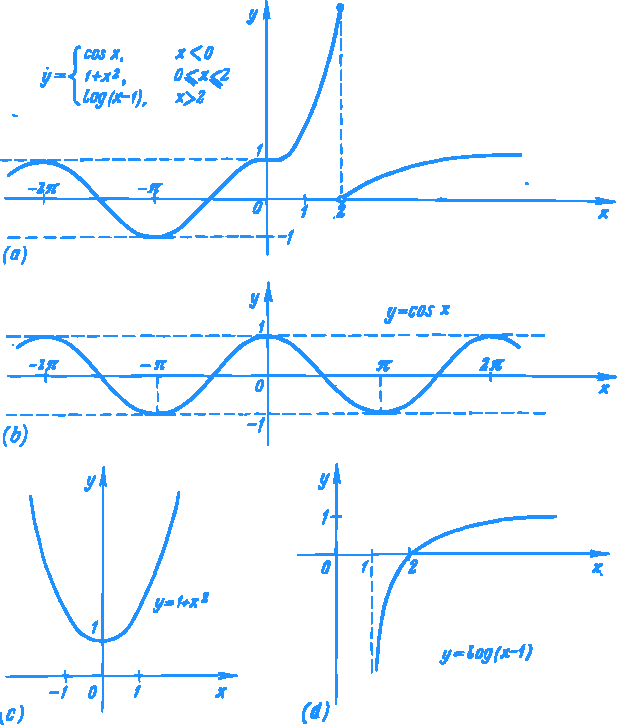
\includegraphics[width=\textwidth]{figures/fig-14.pdf}
\caption{The graphs of the functions $y = \cos x, \, y = 1 +x^{2}$, and $y = \log \, (x -1)$.}
\label{fig-14}
\end{figure}

\rdr In \fig{fig-14}\textcolor{IndianRed}{($a$)} I notice an open circle. What does it mean?

\athr This circle graphically represents a point excluded from the graph. In this particular case the point $(2, 0)$ does not belong to the graph of the function.
\fig{fig-15} plots the graphs of the functions that were discussed at the end of the previous dialogue. Let us have a close look at them.

\begin{figure}[!h]
\centering
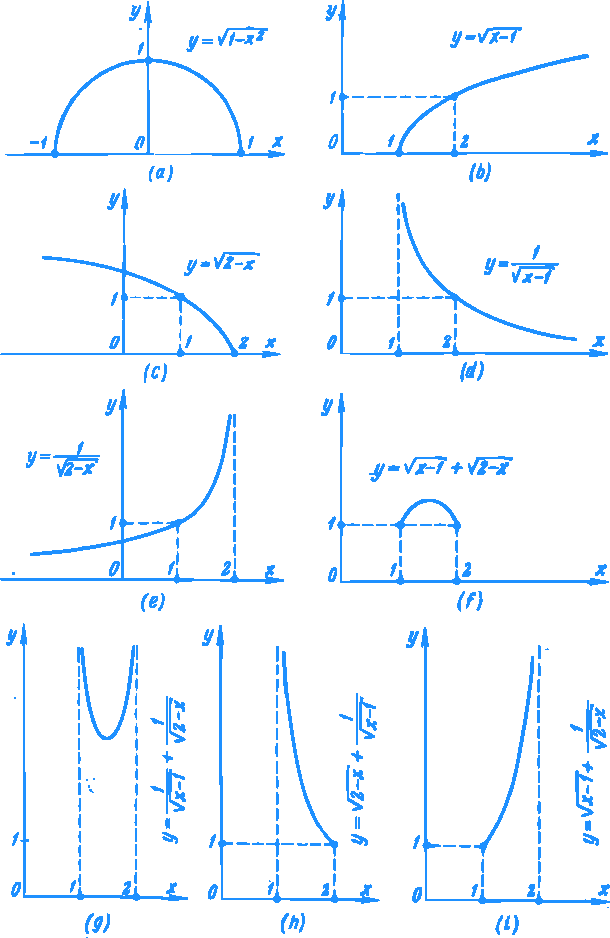
\includegraphics[width=0.85\textwidth]{figures/fig-15.pdf}
\caption{A variety of functions and their domains.}
\label{fig-15}
\end{figure}

\rdr Obviously, in all the cases shown in \fig{fig-15} the domain of the function is supposed coinciding with the domain of the corresponding analytical expression.

\athr Yes, you are right. In cases ($b$), ($c$), ($d$), and ($e$) these domains are infinite intervals. Consequently, only a part of each graph could be shown.

\rdr In other cases, however, such as ($g$), ($h$), and ($i$), the domains of the functions are intervals of finite length. But here as well the figure has space for only a part of each graph.

\athr That is right. The graph is presented in its complete form only in cases ($a$) and ($f$). Nevertheless, the behaviour of the graphs is quite clear for all the functions in \fig{fig-15}.

The cases which you noted, i.e. ($g$), ($h$), and ($i$), are very interesting. Here we deal with the unbounded function defined over the finite interval. The notion of boundedness (unboundedness) has already been discussed with respect
to numerical sequences (see \hyperref[infinite-seq]{Dialogue One}). Now we have to extrapolate this notion to functions defined over intervals.
\begin{mytheo}{Definition}
A function $y = f (x)$ is called \emph{bounded} over an interval $D$ if one can indicate two numbers $A$ and $B$ such that 
\begin{equation*}
A \leqslant f (x) \leqslant B \quad \text{for all $x \in D$} .
\end{equation*}
\end{mytheo}
If not, the function	is called \emph{unbounded}. 

Note that within infinite intervals you may define both bounded and unbounded functions. You are familiar with examples of bounded functions: $y = \sin x$ and $y = \cos x$. Examples of unbounded functions are in \fig{fig-15} (cases ($b$),
($c$), ($d$), and ($e$)).

\rdr Over the intervals of finite length both bounded and unbounded functions may also be defined. Several illustrations of such functions are also shown in \fig{fig-15}: the functions in cases ($a$) and ($f$) are bounded; the functions in cases ($g$), ($h$), and ($i$) are unbounded.

\athr You are right.

\rdr I note that in the cases that I have indicated the bounded functions are defined over the closed intervals ($[-1, 1]$ for ($a$) and $[1, 2]$ for ($f$)), while the unbounded functions are defined both over the open and half-open intervals ($]1, 2[$ for ($g$), $]1, 2]$ for ($h$), and $[1, 2[$ for ($i$)).

\athr This is very much to the point. However, you should bear in mind that it is possible to construct bounded functions defined over open (half-open) intervals, and unbounded functions defined over closed intervals. Here are two simple illustrations:

\textcolor{IndianRed}{\textbf{Example 1:}}  $y= x^{2}  \quad 0 \leqslant x< 2$ \\
\textcolor{IndianRed}{\textbf{Example 2:}}  
\begin{equation*}%
y = 
\begin{cases}
 \dfrac{1}{x} &  0 \leqslant x< 2\\
 1 & x =0
\end{cases}
\end{equation*}

The graphs of these functions are shown in \fig{fig-16}. 
\begin{figure}[!h]
\centering
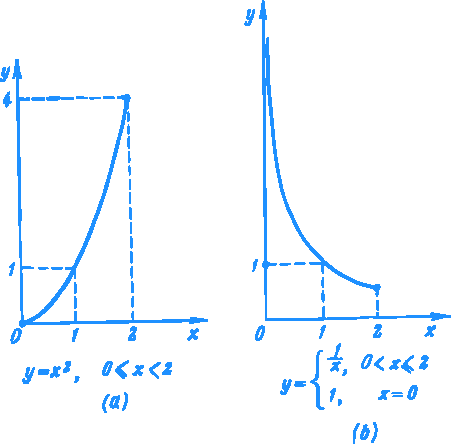
\includegraphics[width=0.75\textwidth,angle=-1]{figures/fig-16.pdf}
\caption{Examples of bounded functions defined over open (half-open) intervals, and unbounded functions defined over closed intervals.}
\label{fig-16}
\end{figure}

\rdr It seems that the boundedness (unboundedness) of a function and the finiteness of the interval over which it is defined are not interrelated, Am I right?

\athr Not completely. There is, for example, the following theorem.
\begin{mytheo}{Theorem}
If a function is defined over a closed interval and if it is monotonic, the function is bounded.
\end{mytheo}
\rdr Obviously, the monotonicity of a function is determined similarly to the monotonicity of a numerical sequence.

\athr Yes, it is. Monotonic functions can be classified, as sequences, into non-decreasing and non-increasing:
\begin{mytheo}{Definition}
\label{monotonic-def}
A function $y = f (x)$ is said to be \emph{non-decreasing} over an interval $D$ it for any $x_{1}$ and $x_{2}$ from this interval $f(x_{1}) \leqslant 
 f(x_{2})$ if $(x_{1} \leqslant  x_{2}$.  If, however, $f(x_{1}) \geqslant 
 f(x_{2})$, the function is said to be \emph{non-increasing}.
\end{mytheo}
Can you prove the theorem formulated above? 

\rdr Let the function $y = f (x)$ be defined over the closed interval $[a, b]$. We denote $f (a) = y_{a}$ and $f (b) = y_{b}$. To make the case more specific, let us assume that the function is non-decreasing. It means that $y_{a} \leqslant y_{b}$. I don't know how to proceed.

\athr Select an arbitrary point $x$ over the interval $[a, b]$.

\rdr Since $a \leqslant x$ and $x \leqslant b$, then, according to the condition of the above theorem, $y_{a} \leqslant f(x)$ and $f(x) \leqslant y_{b}$. Thus, we get that $y_{a}  \leqslant f(x) \leqslant y_{b} $ for all $x$ in the domain of the function. This completes the proof. 

\athr Correct. So, if a \emph{monotonic} function is defined over a closed interval, it is bounded. As to a \emph{non-monotonic} function defined over a closed interval, it may be either
bounded (\fig{fig-15}\textcolor{IndianRed}{($a$)} and ($f$)) or unbounded (\fig{fig-15}\textcolor{IndianRed}{($b$)}). 

And now answer the following question: Is the function $y = \sin x$ monotonic? 

\rdr No, it isn't. 

\athr Well, your answer is as vague as my question. First we should determine the domain of the function. If we consider the function $y = \sin x$ as defined on the natural domain (on the real line), then you are quite right. If, however, the domain of the function is limited to the interval $\left[-\dfrac{\pi}{2}, \dfrac{\pi}{2} \right]$ the function becomes monotonic (non-decreasing).

\rdr I see that the question of the boundedness or monotonicity of any function should be settled by taking into account both the type of the analytical expression for the function and the interval over which the function is defined.

\athr This observation is valid not only for the boundedness or monotonicity but also for other properties of functions. For example, is the function $y = 1 - x^{2}$ an \emph{even} function?

\rdr Evidently the answer depends on the domain of the function.

\athr Yes, of course. If the function is defined over an interval symmetric about the origin of coordinates (for example, on the real line or over the interval $[-1, 1]$), the graph of the function will be symmetric about the straight line $x= 0$. In this case $y= 1- x^{2}$ is an even function. If, however, we assume that the domain of the function is $[-1, 2]$, the symmetry we have discussed above is lost (\fig{fig-17}) and, as a result, $y = 1 - x^{2}$ is not even.
\begin{figure}[!ht]%{r}{0.5\textwidth}
\centering
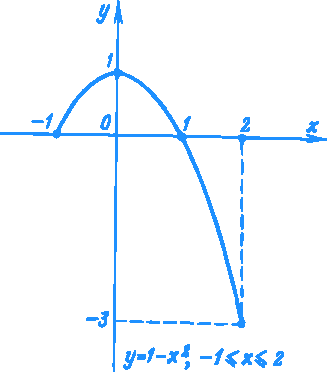
\includegraphics[width=0.5\textwidth,angle=1]{figures/fig-17.pdf}
\caption{ Is the function $y = 1 - x^{2}$  \emph{even}?}
\label{fig-17}
\end{figure}


\rdr It is obvious that your remark covers the case of odd functions as well.

\athr Yes, it does. Here is a rigorous definition of an even function.
\begin{mytheo}{Definition}
A function $y= f (x)$ is said to be \emph{even} if it is defined on a set $D$ symmetric about the origin and if $f (-x) = f (x)$ for all $x \in D$.
\end{mytheo}
By substituting $f (-x) = -f(x)$ for $f (-x) = f (x)$, we obtain the definition of an odd function.

But let us return to monotonic functions. If we drop the equality sign in the definition of a monotonic function (see p.~\pageref{monotonic-def}) (in $f (x_{1}) \leqslant f (x_{2})$ or $f (x_{1}) \leqslant f (x_{2})$), we obtain a so-called \emph{strictly monotonic function}. In this case a non-decreasing function becomes an \emph{increasing function} (i.e. $f (x_{1}) < f (x_{2})$) . Similarly, a non-increasing function becomes a \emph{decreasing function} (i.e. $f (x_{1}) > f (x_{2})$ ). In all the previous illustrations of monotonic functions we actually dealt with strictly monotonic functions (either increasing or decreasing).
\begin{figure}[!h]
\centering
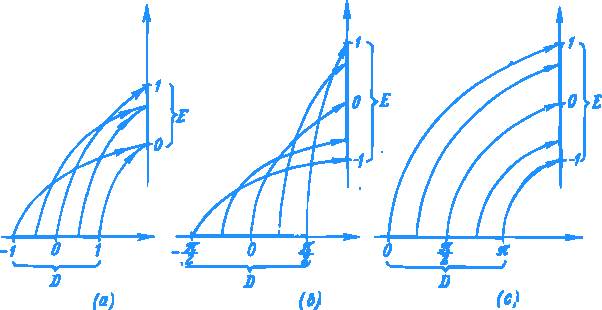
\includegraphics[width=\textwidth]{figures/fig-18.pdf}
\caption{ Concept of an \emph{inverse} function.}
\label{fig-18}
\end{figure}
Strictly monotonic functions possess an interesting property: \emph{each has an inverse function}.

\rdr The concept of an \emph{inverse function} has already been used in the previous dialogue in conjunction with the possibility of mapping a set of equilateral triangles onto a set of circles. We saw that the \emph{inverse mapping}, i.e. the mapping of the set of circles onto the set of equilateral triangles, was possible.

\athr That's right. Here we shall examine the concept of an inverse function in greater detail (but for numerical functions). Consider \fig{fig-18}. Similarly to the graphs presented in \fig{fig-13}, it shows three functions:

\begin{tabular}{lll}
%\begin{enumerate}[label=(\alph*), leftmargin=2cm]
(a) & $y= \sqrt{1-x^{2}}$ & $-1 \leqslant x \leqslant 1$ \\
(b) & $y= \sin x$ &   $- \dfrac{\pi}{2} \leqslant x \leqslant \dfrac{\pi}{2}$\\
(c) & $y= \cos x$ &  0 $\leqslant x  \leqslant  \pi$
%\end{enumerate}
\end{tabular}

Here we have three mappings of one numerical set onto another. In other words, we have three mappings of an interval onto another interval. In case (a) the interval $[-1, 1]$ is mapped onto the interval $[0, 1]$; in (b) the
interval $\left[-\dfrac{\pi}{2}, \dfrac{\pi}{2} \right]$ is mapped onto the interval $[-1, 1]$; and in (c) the interval $[0, \pi]$ is mapped onto the interval $[-1, 1]$.
What is the difference between mappings (b) and (c), on the one hand, and mapping (a), on the other?

\rdr In cases (b) and (c) we have a one-to-one correspondence, i.e. each point of the set $D$ corresponds to a single point of the set $E$ and vice versa, i.e. each point of $E$ corresponds to only one point of $D$. In case (a), however, there is no one-to-one correspondence.

\athr Yes, you are right. Assume now that the directions of all the arrows in the figure are reversed. Now, will the mappings define a function in all the three cases?

\rdr Obviously, in case (a) we will not have a function since then the reversal of the directions of the arrows produces a forbidden situation, namely, one number corresponds to two numbers. In cases (b) and (c) no forbidden situation occurs so that in these cases we shall have some new functions.

\athr That is correct. In case (b) we shall arrive at the function $y = \arcsin x$, which is the inverse function with respect to $y = \sin x$ defined over the interval $\left[-\dfrac{\pi}{2}, \dfrac{\pi}{2} \right]$.

In case (c) we arrive at the function $y =\arccos x$, which is the inverse function with respect to $y = \cos x$ defined over $[0, \pi]$.

I would like to place more emphasis on the fact that in order to obtain an inverse function from an initial function, it is necessary to have a one-to-one correspondence between the elements of the sets $D$ and $E$. That is why the functions $y = \sin x$ and $y = \cos x$ were defined not on their natural domains but over such intervals where these functions are either increasing or decreasing. In other words, the initial functions in cases (b) and (c) in \fig{fig-18} were defined as strictly monotonic. A strict monotonicity is a \emph{sufficient
condition} for the above-mentioned one-to-one correspondence between the elements of $D$ and $E$. No doubt you can prove without my help the following
theorem.
\begin{mytheo}{Theorem}
If a function $y = f(x)$ is strictly monotonic, different $x$ are mapped onto different $y$.
\end{mytheo}
\rdr Thus, a sufficient condition for the existence of the inverse function- is the strict monotonicity of the initial function. Is this right?

\athr Yes, it is.

\rdr But isn't the strict monotonicity of the initial function also a \emph{necessary condition} for the existence of the inverse function?

\athr No, it is not. A one-to-one correspondence may also take place in the case of a non-monotonic function. For example,
\begin{equation*}%
y = 
\begin{cases}
1 - x & 0 < x < 1 \\
x & 1 \leqslant x \leqslant 2
\end{cases}
\end{equation*}
Have a look at the graph of this function shown in \fig{fig-19}. If a function is strictly monotonic, it has the inverse function. However, the converse is not true. 

\begin{figure}[!ht]%[13]{r}{0.5\textwidth}
\centering
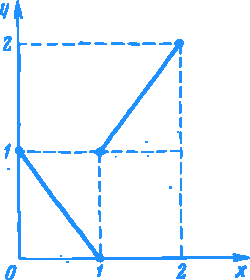
\includegraphics[width=0.48\textwidth]{figures/fig-19.pdf}
\caption{A non-monotonic function.}
\label{fig-19}
\end{figure}

\rdr As I understand it, in order to obtain an inverse function (when it exists), one should simply reverse the roles of $x$ and $y$ in the equation $y = f (x)$ defining the initial function. The inverse function will then be 'given by the equation $x = F (y)$. As a result the range of the initial function becomes the domain of the inverse function.

\athr That is correct. In practice a conversion of the initial function to the inverse function can be easily performed on a graph. The graph of the inverse function is
always \emph{symmetric} to the graph of the initial function about a straight line $y = x$. It is illustrated in \fig{fig-20}, which shows several pairs of graphs of the initial and inverse functions. A list of some pairs of functions with their domains is given below:


\begin{center}
\begin{tcolorbox}[colback=white,colframe=DodgerBlue]
\centering
%\boxed{
$\begin{array}{l>{\color{IndianRed}}cc>{\color{IndianRed}}cc}
\arrayrulecolor{DodgerBlue}
%\hline
 & \textbf{Initial} & \textbf{Domain} & \textbf{Inverse} & \textbf{Domain} \\
 \midrule
(a) & x^{3}& -\infty < x < \infty &\sqrt[3]{x} & -\infty < x < \infty\\
(b) & x^{2} & 0 \leqslant x < \infty & \sqrt{x} & 0 \leqslant x < \infty\\
(c) & 10^{x} & -\infty < x < \infty & \log x &  0 < x < \infty\\
(d) & \sin x & -\dfrac{\pi}{2}  \leqslant x  \leqslant \dfrac{\pi}{2} & \arcsin x & -1 \leqslant x \leqslant 1\\
(e) & \cos x & 0 \leqslant x \leqslant \pi & \arccos x & -1 \leqslant x \leqslant 1\\
(f) & \tan x & -\dfrac{\pi}{2}  < x  < \dfrac{\pi}{2}& \arctan x & -\infty < x < \infty \\
(g) & \cot x & 0 < x < \infty & \text{arccot}\, x &  -\infty < x < \infty\\[5pt]
%\midline
\end{array}$
%}
\end{tcolorbox}
\end{center}



All the domains of the inverse functions shown in the list case of are the natural domains of the functions (however, in the case of $y=\sqrt[3]{x}$ the natural domain is sometimes assumed to be restricted to the interval $[0, \infty[$ instead of the whole real line). As to the initial functions, only two of them ($y = x^{3}$ and $y = 10^{x}$) are considered in this case as defined on their natural domains. The remaining functions are defined over shorter intervals to ensure the strict monotonicity of the functions.

Now we shall discuss the concept of a \emph{composite function}.

Let us take as an example the function $h (x) =\sqrt{1 + \cos^{2} x}$. Consider also the functions $f (x) = \cos x$ and $g (y) = \sqrt{1+y^{2}}$.

\rdr This $f(x)$ notation is something new. So far we used to write $y = f (x)$,

\begin{figure}[!ht]%[13]{r}{0.5\textwidth}
\centering
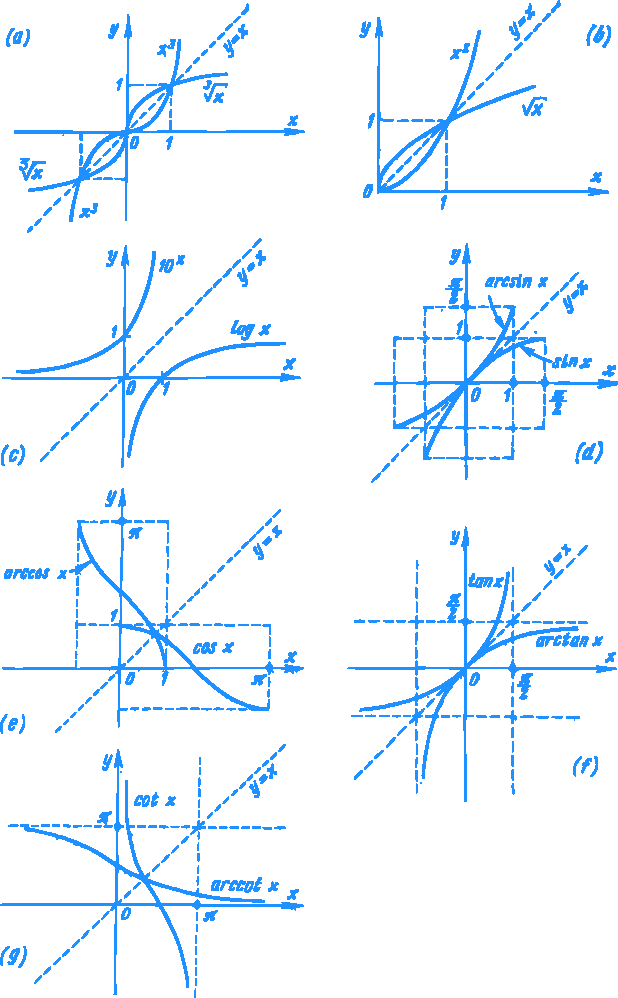
\includegraphics[width=0.85\textwidth]{figures/fig-20.pdf}
\caption{Functions and their inverses showing symmetry along the line $y=x$.}
\label{fig-20}
\end{figure}

\athr You are right. However, it is expedient to simplify the notation.

Consider the three functions: $h (x), \, f (x)$, and $g (y)$. The function $h (x)$ is a composite function composed of $f(x)$ and $g(y)$:
\begin{equation*}%
h (x) = g [f (x)] 
\end{equation*}
\rdr I understand. Here, the values of $f (x)$ are used as the values of the independent variable (argument) for $g (x)$.

\begin{figure}[!ht]%[13]{r}{0.5\textwidth}
\centering
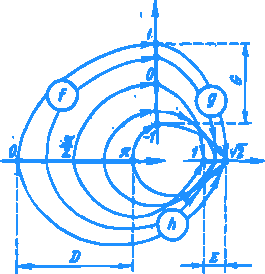
\includegraphics[width=0.5\textwidth]{figures/fig-21.pdf}
\caption{Understanding the composite function.}
\label{fig-21}
\end{figure}

\athr Let us have a look at \fig{fig-21}, which pictures the mappings of sets in the case of our composite function, $h (x) =\sqrt{1 + \cos^{2} x}$, with $f(x) = \cos x$ defined over the interval $[0, \pi]$.

We see that the function $f$ is a mapping of $D$ (the interval $[0, \pi]$) onto $G$ (the interval $[-1, 1]$), that is, the mapping $f$. The function $g$ (the function $\sqrt{1 + y^{2}}$) is a mapping of $G$ onto $E$ (the interval $[1, \sqrt{2}]$), that is, the mapping $g$. Finally, the function $h$ (the function $\sqrt{1 + \cos^{2} x}$ defined over the interval $[0, \pi]$) is a mapping of $D$ onto $E$, that is, the mapping $h$.

The mapping $h$ is a result of the consecutive mappings $f$ and $g$, and is said to be the composition of mappings; the following notation is used
\begin{equation*}%
h = g \circ f
\end{equation*}
(the right-hand side of the equation should be read from right to left: the mapping $f$ is used first and then the mapping $g$).

\rdr Obviously, for a composite function one can also draw a diagram shown in \fig{fig-22}.

\begin{figure}[!ht]%[13]{r}{0.5\textwidth}
\centering
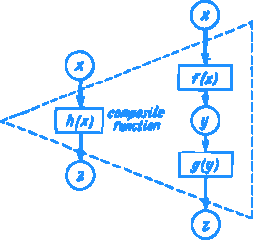
\includegraphics[width=0.5\textwidth]{figures/fig-22.pdf}
\caption{Understanding the composite function.}
\label{fig-22}
\end{figure}


\athr I have no objections. Although I feel that. we better proceed from the concept of a mapping of one set onto another, as in \fig{fig-21}.

\rdr Probably, certain ``difficulties'' may arise because the range of $f$ is at the. same time the domain of $g$? 

\athr In any case, this observation must always be kept in mind. One should not forget that the natural domain of a composite function $g [f (x)]$ is a portion (subset) of the natural domain of $f(x)$ for which the values of $f$ belong to the natural domain of $g$. This aspect was unimportant
in the example concerning $g [f (x)] = \sqrt{ 1 + \cos^{2} x}$ because all the values of $f$ (even if $\cos x$ is defined on the whole real line) fall into the natural domain of $g (y) = \sqrt{1 +y^{2}}$. I can give you, however, a different example:
\begin{equation*}%
h(x) = \sqrt{\sqrt{x-1} -2}, \quad f (x) = \sqrt{x-1}, \quad  g(y)=\sqrt{y -2}
\end{equation*}
The natural domain of $f (x)$ is $[1, \infty[$ Not any point in this interval, however, belongs to the domain of the composite function $h (x)$, Since the expression $\sqrt{y - 2}$ is meaningful only if $y \geqslant 2$, and for $y = 2$ we have $x = 5$, the natural domain of this composite function is represented by $[5, \infty]$, i.e. a subset smaller than the natural domain of $f (x)$.

Let us examine one more example of a composite function. Consider the function $y = \sin \,(\arcsin x)$, You know that $\arcsin x$ can be regarded as an angle the sine of which is equal to $x$. In other words, $\sin(\arcsin x) = x$, Can you point out the difference between the composite function $y = \sin \, (\arcsin x) $ and the function $y = x$?

\rdr Yes, I can. The natural domain of the function $y = x$ is represented by the whole real line. As to the composite function $y = \sin (\arcsin x)$, its natural domain coincides with the natural domain of the function $\arcsin x
$, i.e. with $[-1, 1]$. The graph of the function $y = \sin (\arcsin x)$ is shown in \fig{fig-23}.
\begin{figure}[!ht]%[13]{r}{0.5\textwidth}
\centering
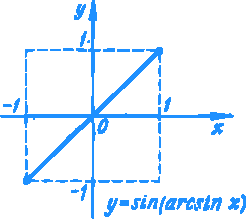
\includegraphics[width=0.5\textwidth]{figures/fig-23.pdf}
\caption{The graph of the function $y = \sin (\arcsin x)$.}
\label{fig-23}
\end{figure}

\athr Very good. In conclusion, let us get back to the problem of the graphical definition of a function. Note that there are functions whose graphs cannot be plotted in principle, the whole curve or a part of it. For example, it is impossible to plot the graph of the function $y= \sin \dfrac{1}{x}$ in the vicinity of $x = 0$ (\fig{fig-24}). It is also impossible to have the graph of the Dirichlet	function mentioned above.
\begin{figure}[!ht]%[13]{r}{0.5\textwidth}
\centering
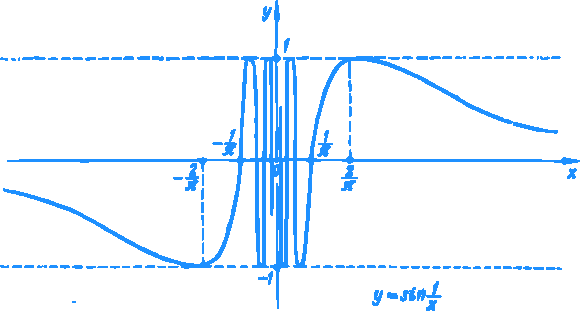
\includegraphics[width=\textwidth]{figures/fig-24.pdf}
\caption{The graph of the function $y = \sin \dfrac{1}{x}$.}
\label{fig-24}
\end{figure}

\rdr It seemed to me that the Dirichlet function had no graph at all. 

\athr No, this is not the case. Apparently, your idea of a graph of a function is always a curve.

\rdr But all the graphs that we have analyzed so far were curves, and rather smooth curves, at that.

\athr In the general case, such an image is not obligatory. But it should be stressed that \emph{every function has its graph, this graph being unique}.

\rdr Does this statement hold for functions that are not numerical

\athr Yes, it does. In the most general case we can give the following definition.
\begin{mytheo}{Definition}
The graph of a function $f$ defined on a set $D$ with a range on a set $E$ is a set of all pairs $(x, y)$ such that the first element of the pair $x$ belongs to $D$, while the second element of the pair $y$ belongs to $E$, $y$ being a function of $x \,\, (y= f(x))$.
\end{mytheo}

\rdr So it turns out that the graph of a function such as the area of a circle is actually a set of pairs each consisting of a circle (an element $x$) and a positive number (an element $y$) representing the area of a given circle.

\athr Precisely so. Similarly, the graph of a function representing a schedule of students on duty in a classroom is a set of pairs each containing a date (an element $x$) and the name of a student (an element $y$) who is on duty on this date. Note also that in practice this function indeed takes a graphic form.

If in a particular case both elements of the pair (both $x$ and $y$) are numbers, we arrive at the graph of the function represented by a set of points on the coordinate plane. This is the familiar graph of a numerical function.
}